\documentclass[a4paper,11pt,openright,english,twoside]{report}
%\usepackage[T1]{fontenc}     			             		% font encoding
%\usepackage[utf8]{inputenc} 			          		% input encoding
%\usepackage{subcaption}
% use paper rather more fully
\usepackage{fullpage}
%\usepackage{savetrees}  % extreme: for drafts

% use paper rather more fully
\usepackage{fullpage}
%\usepackage{savetrees}  % extreme: for drafts

% versatile multi-column environment
\usepackage{multicol}
\usepackage{multirow} % for making tables 
\usepackage{textpos}

%chem package
\usepackage[version=3]{mhchem}
% extra general symbols
\usepackage{latexsym}
%\usepackage[style=numeric]{biblatex}
% extra maths capabilities
\usepackage{amsmath}
\usepackage{amsthm}
\usepackage{amsfonts}
\usepackage{amssymb}
\usepackage{mathrsfs}
\usepackage{color}
\usepackage{multirow}

% KTH colors
% site:
% {0.435294118,0.647058824,0.831372549}
% {0.88627451,0.88627451,0.88627451}
% {0.705882353,0.784313725,0.882352941}
% {0.666666667,0.717647059,0.8}
% {0.866666667,0.866666667,0.866666667}
\usepackage[	
	author={Kartik Karuna},						% author
	title={Optimized MPPT implementation for Dye-sensitized Solar cells},			 %title
	subtitle={Maximum Power Point Tracking for DCSs},	 % subtitle
    date={\today},
]{thesis}

\begin{document}

	%\include{chapters/00_title}
	\makeititle
	
	\pagenumbering{roman}
	\pagestyle{begin}		% bug on tocloftpagestyle
	
	\pdfbookmark{Sammanfattning}{Sammanfattning}
\chapter*{Sammanfattning}
\thispagestyle{begin}

\begin{tabular}{ | p{\dimexpr \linewidth-2\tabcolsep} |} \hline
 \begin{figure}[H]
        
        
\includegraphics[width=0.2\textwidth]{images/indust} 
             \end{figure}  \\\hline
\end{tabular}   
\begin{tabular}{ | p{\dimexpr 0.3424\linewidth-2\tabcolsep} |
                  p{\dimexpr 0.3424\linewidth-2\tabcolsep} |
                  p{\dimexpr 0.3424\linewidth-2\tabcolsep} |} \hline
                 Godkänt & Examinator & Handledare \\
                  \textbf{2015-MM-DD}  & \textbf{Martin Törngren} & \textbf{Baha Hasan} \\\hline
                   & Uppdragsgivare & Kontaktperson \\
                   & \textbf{EXEGER Sweden AB} & \textbf{Camila Niva}\\ \hline
\end{tabular} \\
\begin{textblock}{8}(3,-3.3)
\begin{center}
\textbf{Examensarbete MMK 2014: MF212X }
\end{center}
\end{textblock}
\begin{textblock}{8}[0.5,0.5](7,-2.3)
\begin{center}
\textbf{Optimized MPPT implementation for Dye-sensitized Solar cells}
\end{center}
\end{textblock}
\begin{textblock}{5}(8,-1.5)
Kartik Karuna
\end{textblock}
% Here the abstract, remove the following command

 European Commission's roadmap for moving to a low-carbon economy calls for a drastic reduction in the use of carbon based fuels.A low-carbon economy would have a much greater need for renewable sources of energy, energy-efficient building materials and other related technologies in order to reach its goals by 2050.More locally produced energy would be used, mostly from renewable sources with solar and wind playing an every increasing role.
 Energy efficiency will be a key driver of the transition.



{\bf Nyckelord:} DSCs, MPPT, PnO, INC, Golden Search Algorithm, Machine Learning. 
\acresetall

	\pdfbookmark{Abstract}{Abstract}

\chapter*{Abstract}


\begin{tabular}{ | p{\dimexpr \linewidth-2\tabcolsep} |} \hline
 \begin{figure}[H]
        
        
\includegraphics[width=0.2\textwidth]{images/indust} 
             \end{figure}  \\\hline
\end{tabular}   
\begin{tabular}{ | p{\dimexpr 0.3424\linewidth-2\tabcolsep} |
                  p{\dimexpr 0.3424\linewidth-2\tabcolsep} |
                  p{\dimexpr 0.3424\linewidth-2\tabcolsep} |} \hline
                 Approved & Examiner & Supervisor \\
                  \textbf{2015-MM-DD}  & \textbf{Martin Törngren} & \textbf{Baha Hasan} \\\hline
                   & Commissioner & Contact person \\
                    & \textbf{EXEGER Sweden AB} & \textbf{Camila Niva}\\ \hline
\end{tabular} \\

\begin{textblock}{8}(3,-3.3)
\begin{center}
\textbf{Master of Science Thesis MMK 2014: MF212X }
\end{center}
\end{textblock}
\begin{textblock}{8}[0.5,0.5](7,-2.3)
\begin{center}
\textbf{Optimized MPPT implementation for Dye-sensitized Solar cells}
\end{center}
\end{textblock}
\begin{textblock}{5}(8,-1.5)
Kartik Karuna
\end{textblock}
% Here the abstract, remove the following command

 European Commission's roadmap for moving to a low-carbon economy calls for a drastic reduction in the use of carbon based fuels. A low-carbon economy would have a much greater need for renewable sources of energy, energy-efficient building materials and other related technologies in order to reach  goals by 2050. More locally produced energy would be used, mostly from renewable sources with solar and wind playing an ever increasing role.Energy efficiency will be a key driver of this transition. Designing self-powered devices could offset a huge portion of the carbon budget, freeing devices from charging and making them truly wireless. \\
 
  Dye-Sensitized Solar Cells (DSCs) owing to their low-cost manufacturing technique among other advantages, could well be the missing piece in this puzzle. Lower efficiency vis-à-vis its Silicon based counterparts have dithered large scale implementation, however, with continued research that is soon to change. In order to  maximize the produced energy, several maximum power point tracking (MPPT) algorithms have been proposed and developed over the years. They vary in implementation, energy efficiency, convergence speed, sensors required, cost effectiveness etc. Although comparative studies, based on widely-adopted MPPT algorithms, have been presented before they focused on commercially available Silicon based Solar-cells; none have applied their findings to DSCs in indoor conditions. This work presents an experimental comparison, under simulated indoor irradiation, of three most used MPPT methods for PV power systems in an attempt to find one most suitable for DSCs. Subsequent experiments showed the existing MPPT methods to be unsuitable for DSCs leading to a new hybrid Algorithm being proposed.\\       

{\bf Keywords:} DSCs,Grätzel cells, MPPT, PnO, INC, Golden Search Algorithm, Machine Learning. 
\acresetall

	\pdfbookmark{Acknowledgements}{Acknowledgements}
\chapter*{Acknowledgments}
\thispagestyle{begin}

% here the acknlowledgments

text text text text text text text text text text text text text text text text text text text text text text text text text text text text text text text text text text text text text text text text text text text text text text text text text text text text text text text text text text text text text text text text text text text text text text  \\

insert text here insert text here insert text here insert text here insert text here
insert text here insert text here insert text here insert text here insert text here insert text here insert text here insert text here insert text here insert text here insert text here insert text here insert text here insert text here insert text here insert text here insert text here insert text here insert text here insert text here insert text here insert text here insert text here insert text here   \\

insert text here insert text here insert text here insert text here insert text here
insert text here insert text here insert text here insert text here insert text here insert text here insert text here insert text here insert text here insert text here insert text here insert text here insert text here insert text here insert text here insert text here insert text here insert text here insert text here insert text here insert text here insert text here insert text here insert text here   \\

	\clearpage
	\tableofcontents
	\clearpage
	\listoffigures
	%\listoftables
	
	% acronym list
	\chapternotoc{Acronyms}

\begin{acronym}[YOURLONGESTACRONYM]

	 \acro{DSCs}{Dye-Sensitized Solar Cells}
	 \acro{MPPT}{Maximum Power Point Tracking}
	 \acro{ADC}{Analog to Digital Converter}
	 \acro{DAC}{Digital to Analog Converter}
	 \acro{PV}{Photo–voltaic}
	 \acro{CdTe}{Cadmium telluride}
	 \acro{CIGS}{Copper-indium-gallium selenide}
	 \acro{CIS}{Copper-indium sulphide}
	 \acro{a-Si}{Amorphous silicon}
	 \acro{MPP}{Maximum Power Point}
	 \acro{PnO}{Perturb and Observe}
	 \acro{FOCV}{Fractional Open Circuit Voltage}
	 \acro{ICM}{Incremental Conductance Method}
	 \acro{FTO}{Fluorine-doped tin oxide}
	 \acro{WE}{Working Electrode}
	 \acro{CE}{Counter Electrode}
	 \acro{HOMO}{Highest Occupied Molecular Orbital}
	 \acro{LUMO}{Lowest Unoccupied Molecular Orbital}
	 \acro{F.F}{Fill Factor}
	 \acro{GSSA}{Golden Section Search Algorithm}
	 \acro{LED}{Light Emitting Diode}
	 \acro{SMU}{Source-Measure Unit}
	 \acro{VAL}{Voltage approximation line}
	 \acro{FIFO}{First In First Out}
	 \acro{DSP}{Digital Signal Processor}
	 \acro{HIL}{Hardware In the Loop}
	 

\end{acronym}


	\cleardoublepage
	\pagenumbering{arabic}
	\setcounter{page}{1}

	\pagestyle{main}

	\pdfbookmark{Introduction}{Introduction}
\chapter{Introduction}
\begin{quote} 
\it This chapter gives a basic introduction to  \ac{DSCs} and \ac{MPPT}.It also defines the scope, Goals, Objective and the Research Methodology for the thesis.
\end{quote}

\section{Background}

Our ever increasing reliance on electrical and electronic equipment intensified our search for new sources of energy. Dwindling fossil-fuel reserves are not something we can rely on in the long-term.Alternate energy sources must be efficient,cost-effective and ecologically friendly.The Harnessing of solar energy becomes a very attractive proposition.A moderately efficient solar cell array (8\%-10\% efficiency) Covering a small portion of the earth's surface would be able to provide an enormous amount of electric power and thus reduce greenhouse-gas emissions \cite{kalyanasundaram2010dye}. However, the current high cost of solar panels made from traditional inorganic semiconductors imposes a restriction on their mass usage.
 **picture about the losses  Solar energy intercepting Earth [toivola2010dye]**
 
 \subsection{Dye-Sensitized Solar Cells(DSCs)}
  Photovoltaic devices are based on the concept of charge separation at an interface of two materials of different conduction mechanism. To date this field has been dominated by solid-state junction devices, usually made of silicon, and profiting from the experience and material availability resulting from the semiconductor industry. The dominance of the photovoltaic field by inorganic solid-state junction devices is now being challenged by the emergence of a third generation of cells, based, e.g. on nano-crystalline oxide and conducting polymers films \cite{gratzel2004conversion}. Crystalline silicon being the first; and thin film technologies such as \ac{CdTe}, \ac{CIGS}, \ac{CIS} and \ac{a-Si} being examples of the second generation \cite{toivola2010dye}.\\
  
  Solar energy can be converted into electricity by a variety of technologies that can also be divided into four classes: Concentrator systems, wafer-based crystalline silicon, thin-film technologies, and emerging technologies\cite{wenger2010strategies}.\\
  
    \begin{figure}[H]
    \begin{center}
    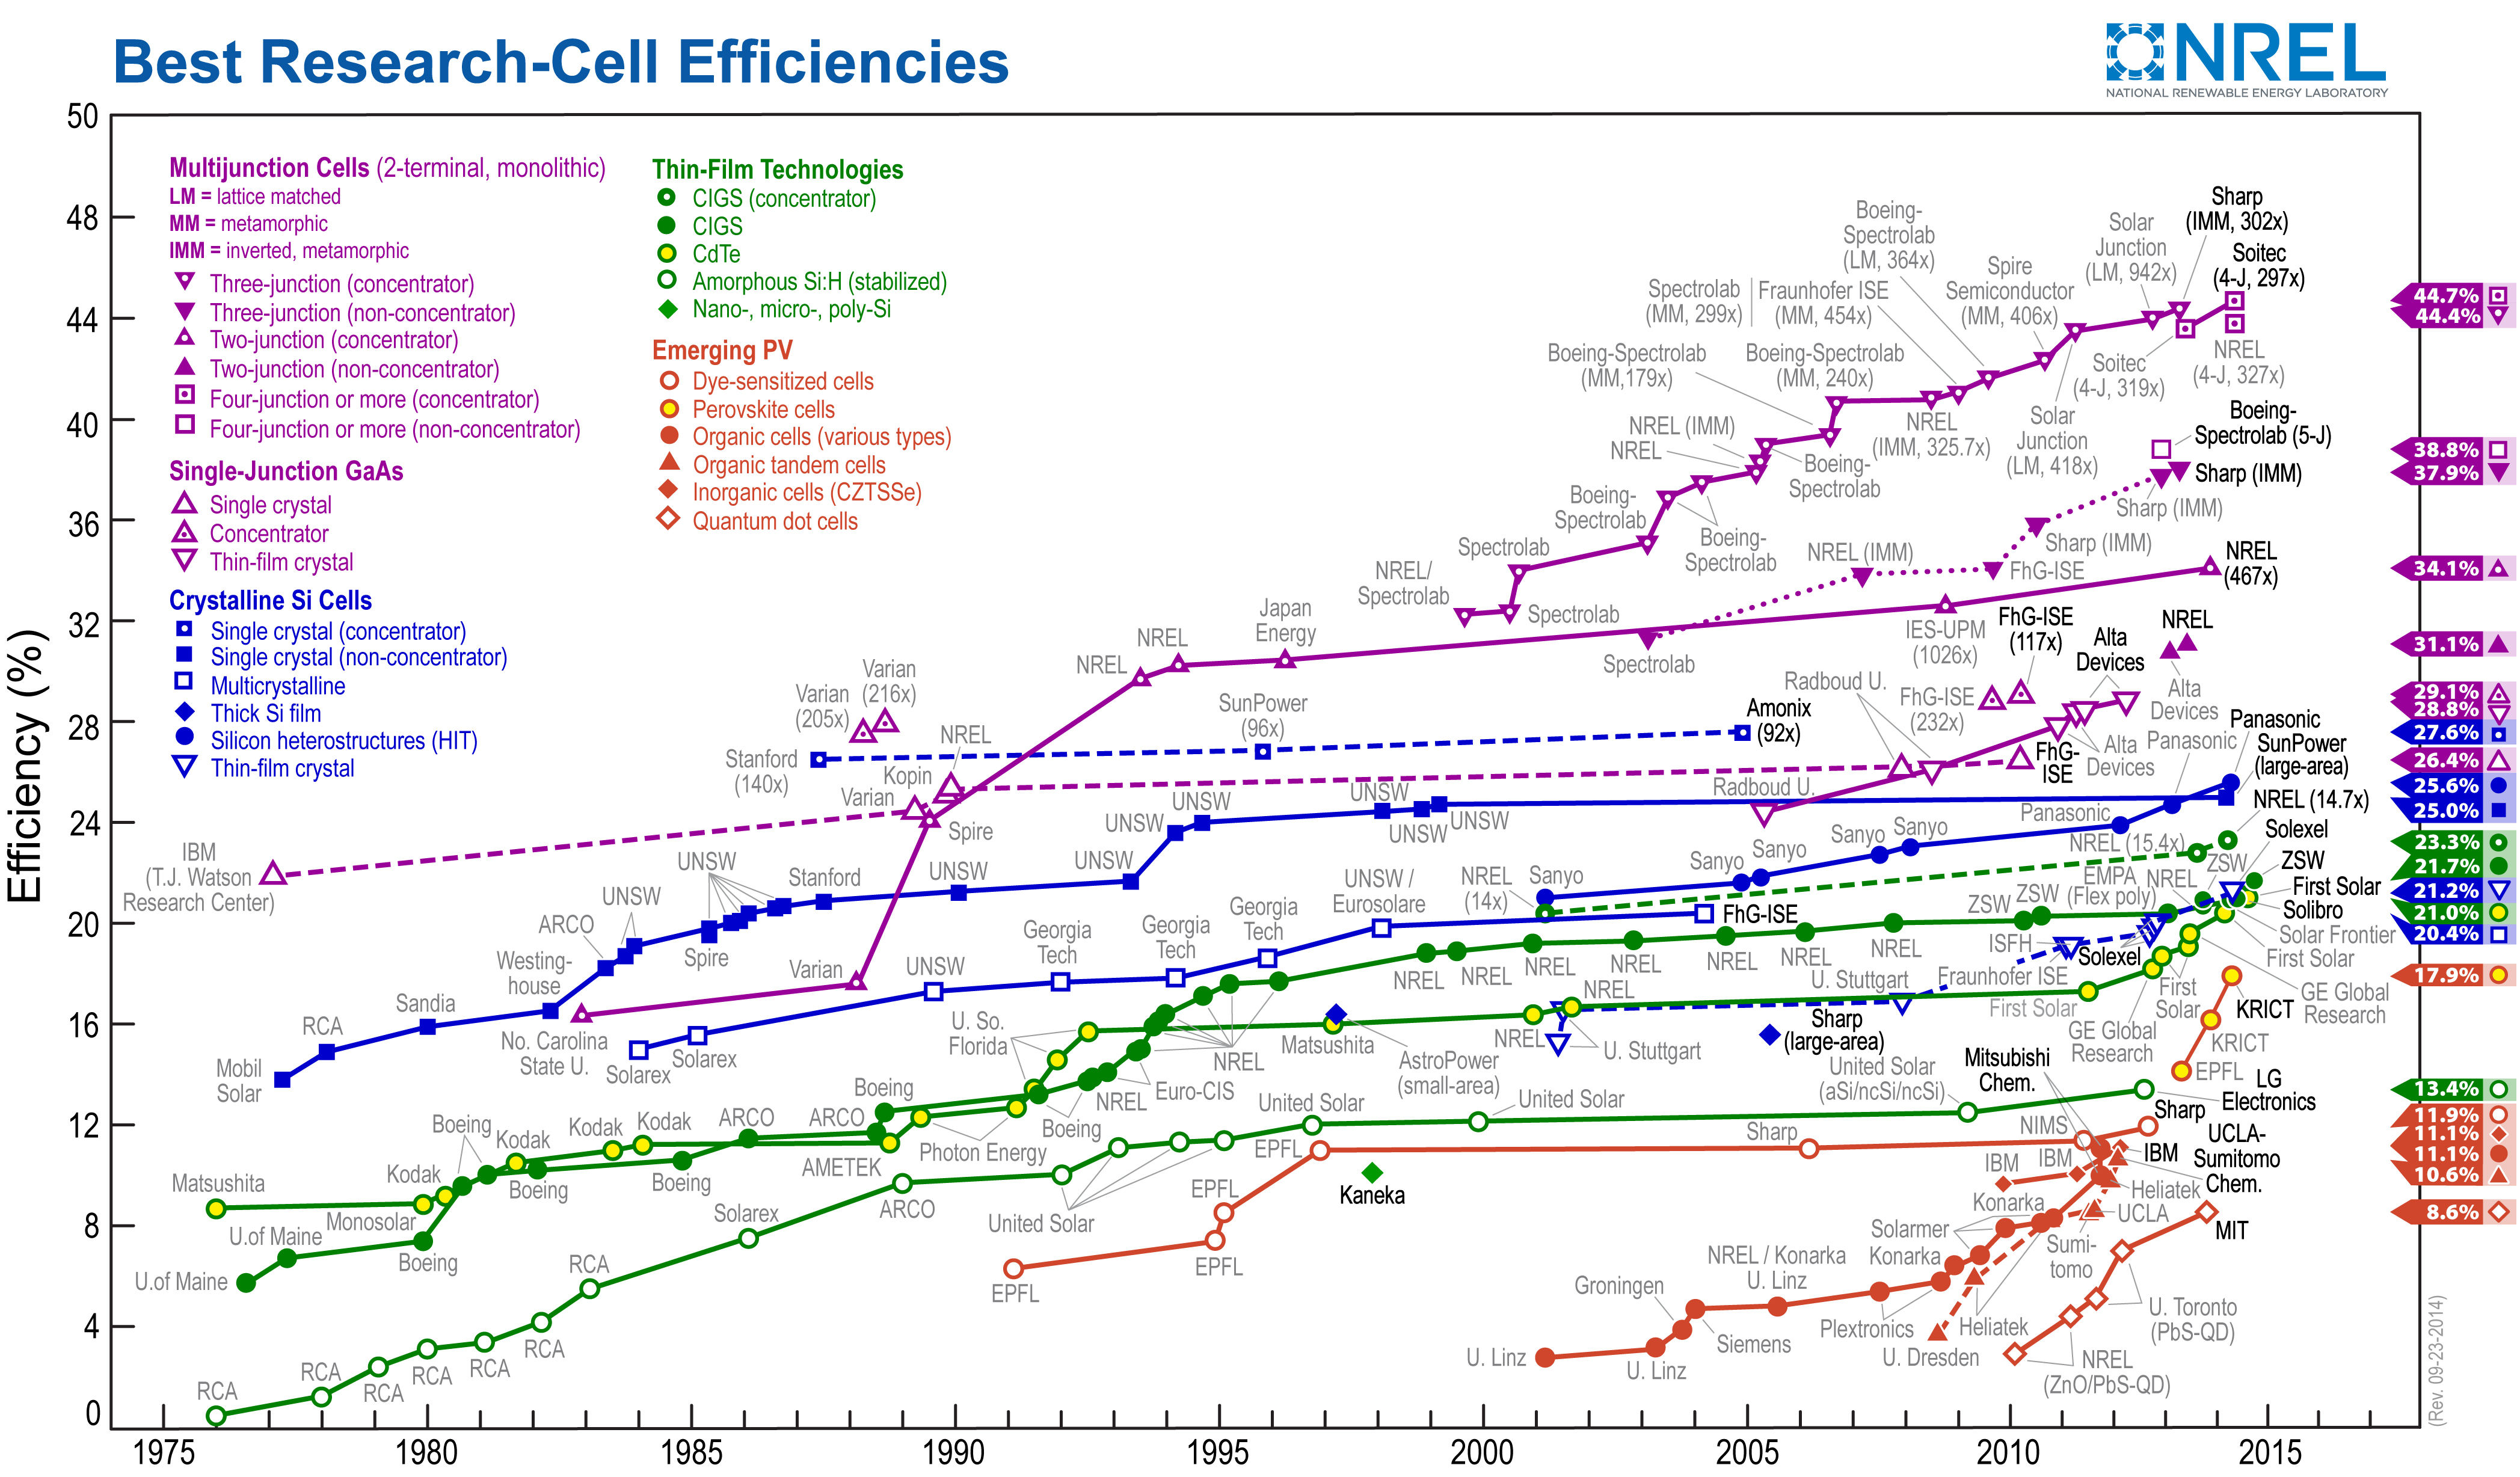
\includegraphics[width=\textwidth]{images/efficiency_chart.jpg}
    \caption{Research Cell Efficiency Records \cite{nrel_Research_Cell} }
    \label{fig:Cell_eficency}
    \end{center}
    \end{figure}
  
  Dye-sensitized solar cells(\ac{DSCs}) are the most promising of the third and latest generation of solar cells. Under development for the last 20 years, this technology is ready for large scale commercialization to provide robust, efficient, and affordable solar energy to the masses. unlike previous generation cells, \ac{DSCs} is a Photo-electro-chemical device whose principal of operation is similar to Photosynthesis seen in plants.\\

 \subsection{Advantages of DSCs }
  
  The *** of solar cells is slow **.A major contributing factor for this is the predominant type of solar cells used today -ones made from silicon, which are quite expensive and are complex to manufacture. This has lead to intensive research in to alternative solar cells in the past decade. \ac{DSCs} have many advantages over their 1st and 2nd generation counterparts. They offer transparency, low cost, and high power conversion efficiencies under cloudy and artificial light conditions.\ac{DSCs} work even in low-light conditions such as non-direct sunlight and cloudy skies.They are easy and economical to manufacture,with the major constituent materials available in abundance in most counties. **This availability of Raw material also enables us to scale the manufacturing to Tera-Watts levels relatively simple.Since raw-materials are non-toxic and there are no noxious emissions during manufacturing-Sustainable**\\
  
   
  \begin{figure}[H]
  \begin{center}
  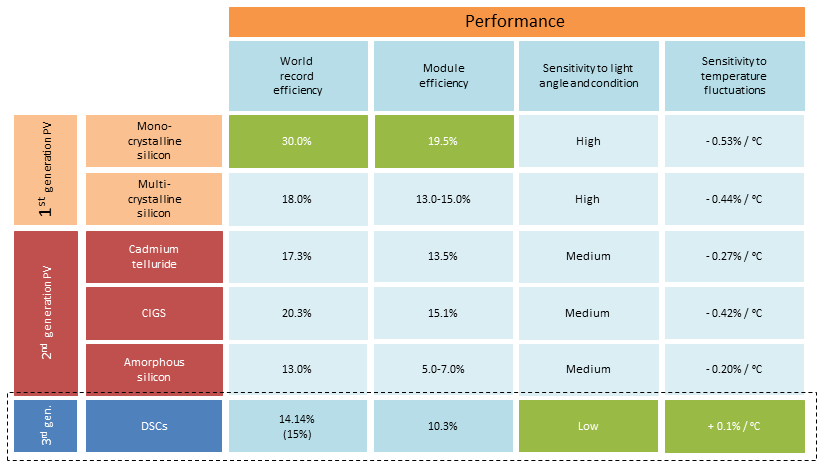
\includegraphics[width=\textwidth]{images/3rd_gen}
  \caption{ Three generations of cells –  Performance}
  \label{fig:3rd_gen}
  \end{center}
  \end{figure}
 
  **Add more details about Advantage of DSC over conventional cells **\\
 
   
\section{Maximum power Point Tracking(MPPT)}

A photovoltaic (PV) array that functions under uniform radiation and temperature conditions presents an I–V and P–V characteristic as the one shown in Figure ~\ref{fig:IVgraph} and Figure ~\ref{fig:PVgraph},respectively. As can be observed, there is a single point, called \ac{MPP}, where the array provides the maximum power possible for these environmental conditions (radiation and temperature), and so functions with the maximum performance. When a load is connected directly to a PV array (direct coupling), the operation point is defined by the intersection of its I–V characteristics, as shown in Figure ~\ref{fig:IVgraph}. In general, this operation point does not coincide with the \ac{MPP}. Thus, in direct coupling systems, the array must be over-dimensioned to guarantee the power demand of the load. Obviously, this implies a more expensive system. To solve this problem, a DC/DC  converter with an algorithm for the automatic control of its duty cycle “${\delta}$” is inserted between the photovoltaic array and the load , resulting in what is known as \ac{MPPT} system. The MPPT must control the voltage or current (through the ${\delta}$ the converter) of the PV array regardless of the load, trying to place it in the \ac{MPP}.Therefore,the MPPT must find the optimal ${\delta}$ for the operation point of the PV array to coincide with the \ac{MPP}\cite{enrique2010reliable}.\\

Although the solution to operating in the \ac{MPP} may seem straightforward, it is not. This is because the location of the \ac{MPP} in the I–V curve of the PV array is not known beforehand. This point must be located, either by mathematical calculations over a valid model, or by using some search algorithm. This implies even more difficulty if we consider the fact that the \ac{MPP} presents non-linear dependencies with temperature and radiation\cite{enrique2010reliable}\\





  \begin{figure}[H]
  \begin{center}
  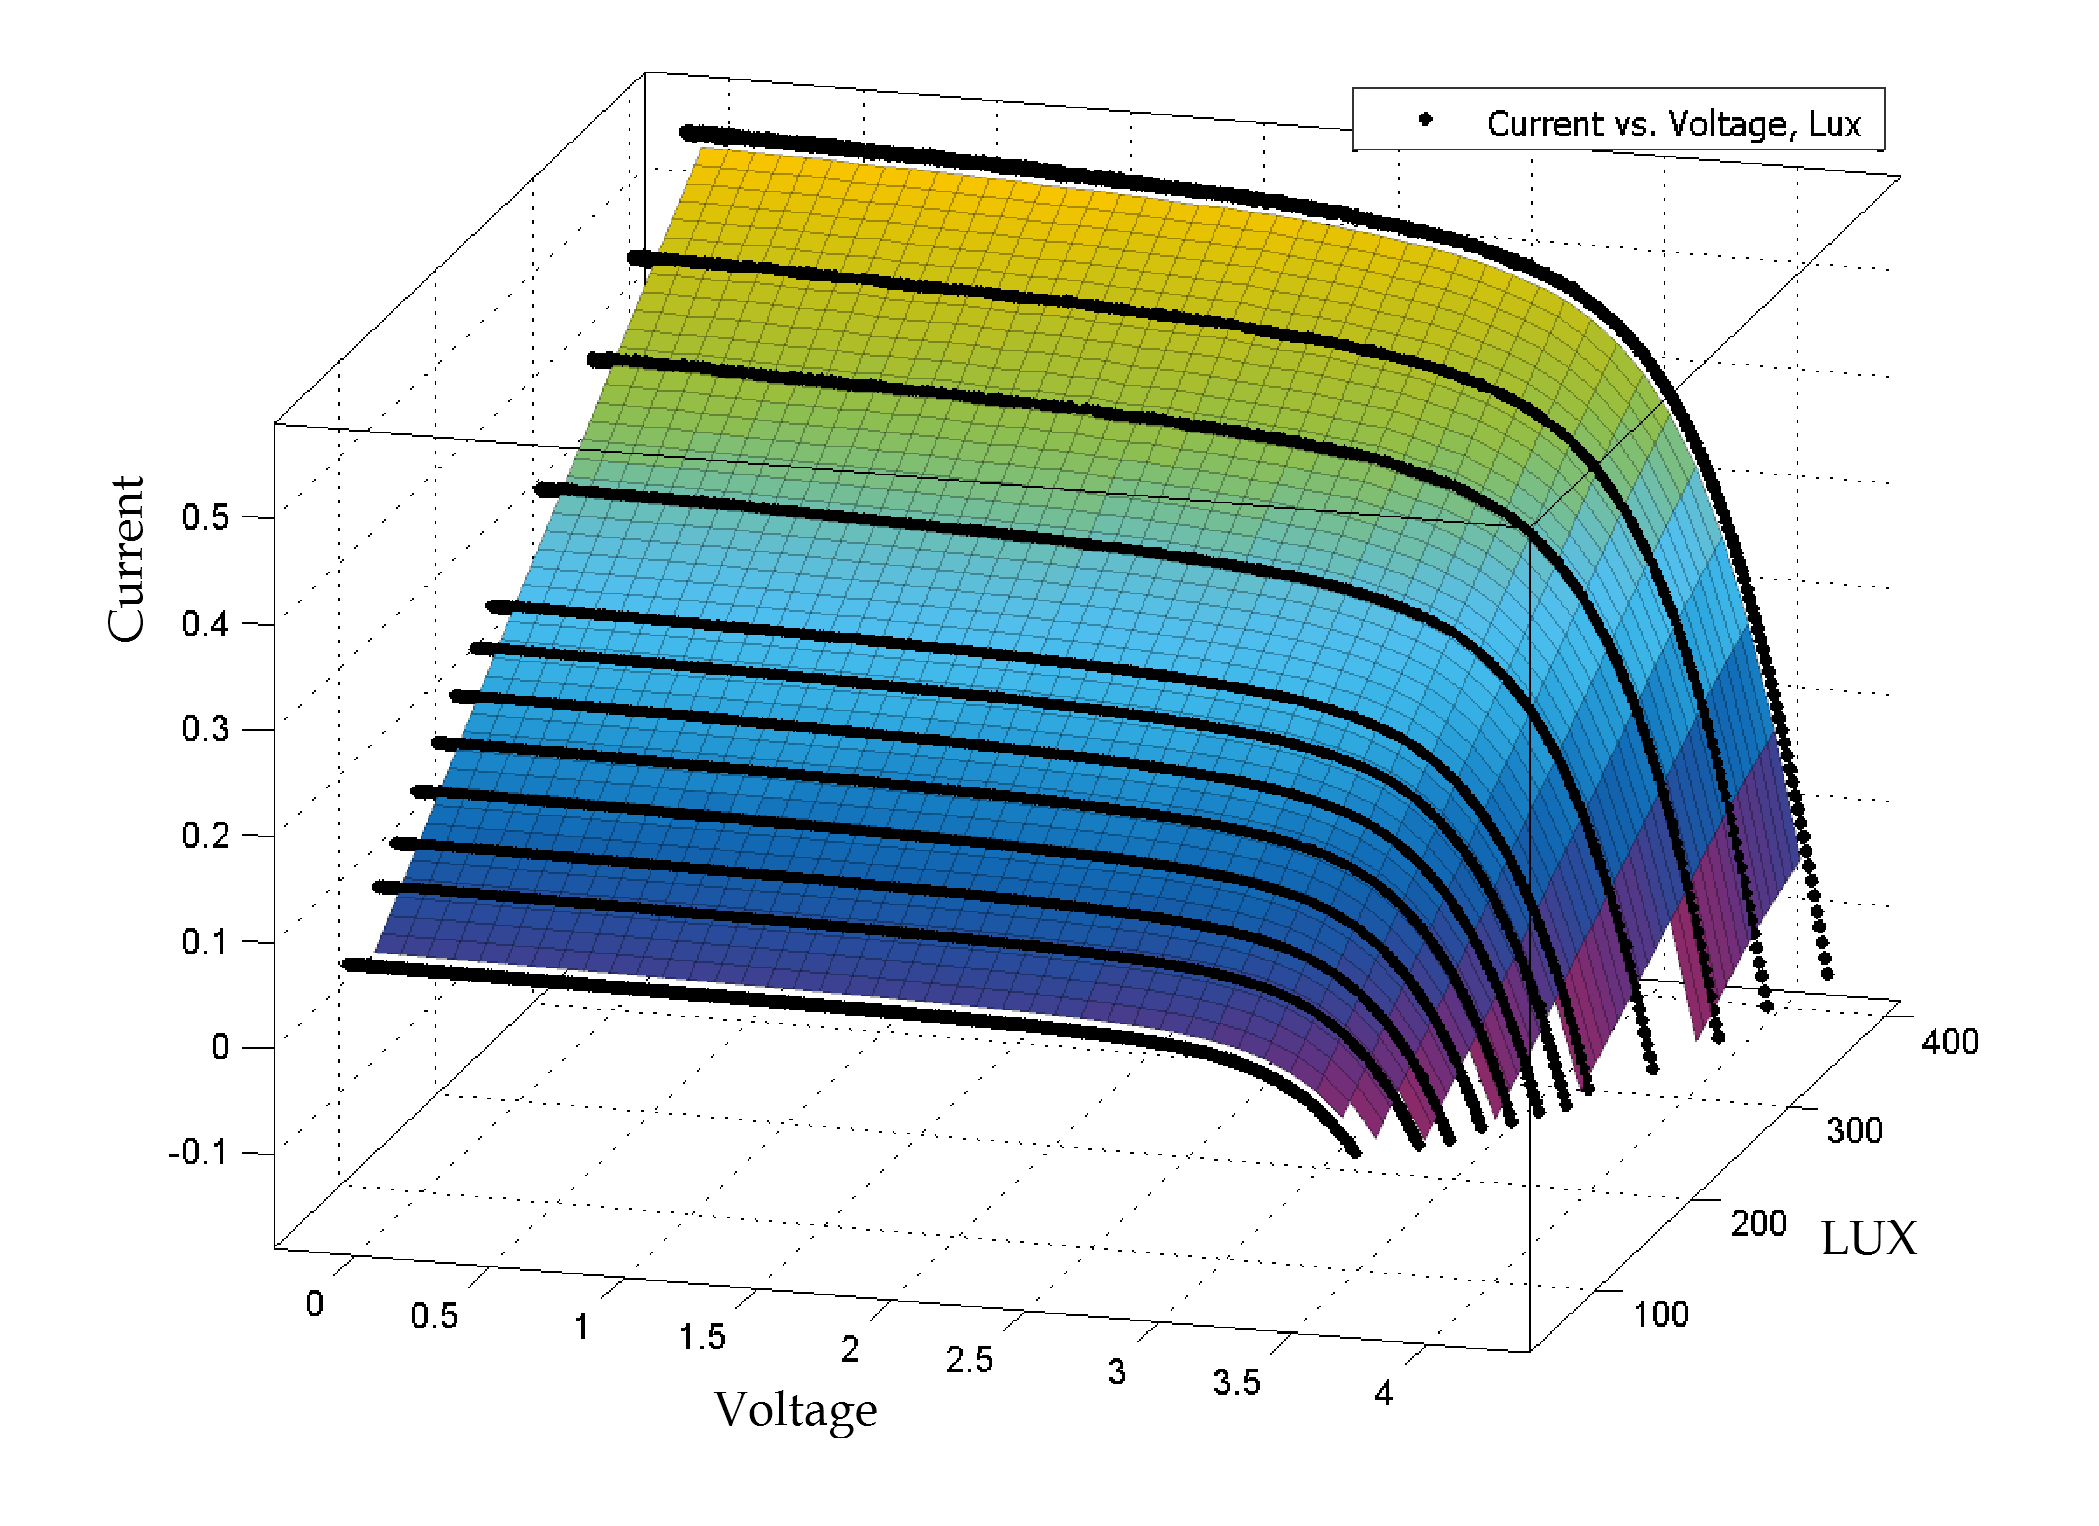
\includegraphics[width=\textwidth]{images/I-V-lux}
  \caption{I-V-Lux}
  \label{fig:IVgraph}
  \end{center}
  \end{figure}
  
    \begin{figure}[H]
    \begin{center}
    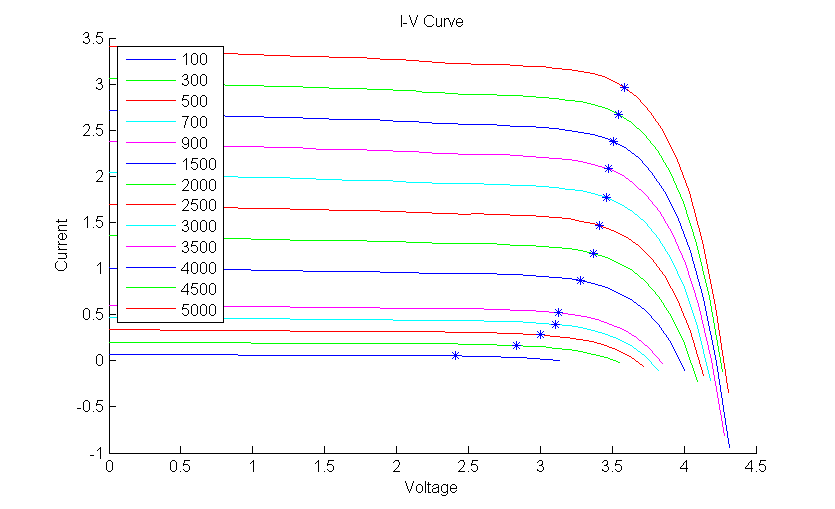
\includegraphics[width=\textwidth]{images/IV_lux_MPP}
    \caption{I-V Graph, MPPT marked with '*'}
    \label{fig:IV_mppgraph}
    \end{center}
    \end{figure}
  
  \begin{figure}[H]
  \begin{center}
  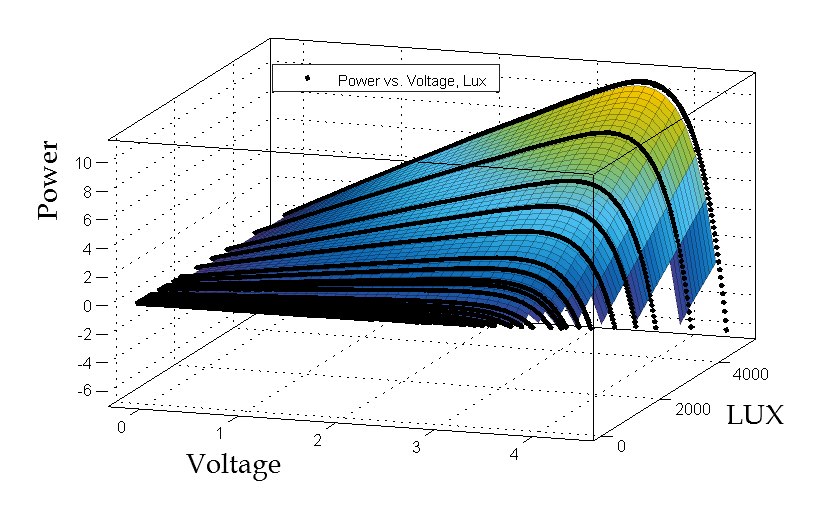
\includegraphics[width=\textwidth]{images/PV_LUX}
  \caption{ P-V Lux}
  \label{fig:PVgraph}
  \end{center}
  \end{figure}

As such, Numerous \ac{MPPT} methods have been developed and implemented\cite{ngan2011study} \cite{esram2007comparison} \cite{eltawil2013mppt} . The methods vary in complexity, sensors required, convergence speed, cost, range of effectiveness, implementation hardware, popularity, and in other respects\cite{reza2013classification} \cite{dondi2008modeling}. They range from the almost obvious (but not necessarily ineffective) to the most creative (not necessarily most effective). In fact, so many methods have been developed that it has become difficult to adequately determine which method, newly proposed or existing, is most appropriate for a given PV system.Some of the most popular being: \\

  
\begin{itemize}
 \item Perturb and Observe Method
 \item Incremental Conductance Method
 \item fractional open circuit voltage Method
 \item Fixed duty cycle Method
 \item Pilot cell Method
 \item Pilot cell Method
 \item Fractional short-circuit current Method
 \item Fuzzy logic controller
\end {itemize}
 
 
 
\section{Scope, Thesis Goals and Objectives}

This thesis focuses on the finding a practically **optimal** and usable \ac{MPPT} algorithm that is optimised to be used with the current \ac{DSCs}.\\


The objectives of the thesis can be summarized as:
\begin{itemize}

\item Develop an Electrical model for DSCs and verify the accuracy of said model.
 
\item Compare and optimize the following Maximum power point tracking (MPPT) algorithms for compatibility with the above Model using MATLAB{\textregistered} and Simulink{\textregistered}.
	\begin{enumerate}
		\item \ac{PnO} Method.
		\item \ac{ICM}.
		\item \ac{FOCV} Method.
		
	\end{enumerate}
\item Setting up the test environment   
\item Execution of test cases on prototype developed, based on two of the best optimized algorithm, with recordable test results.
\item Develop Reference designs for production.
\item Internal report.
\item  Master thesis report. 
\end {itemize}

\section{Thesis outline}
\begin{itemize}
\item Chapter 1 Presents the background and the main objectives of this thesis \\
\item Chapter 2 Contains the prior research and literature that this thesis was based on, it also discusses the principle of operating principles/state-of-the-art  of \ac{DSCs} and of \ac{MPPT} \\
\item Chapter 3 concerns the  research methods, measurement techniques and implementation of the thesis.
\item Chapter 4 Gives a summary of the results. 
\item The thesis is Concluded and Future Work talked about in Chapter 5
\end {itemize}

\section{Research Methodology}
The implementation of the thesis is ** 
\begin{itemize}
\item Develop a suable model for the \ac{DSCs} based on either:.
	\begin{enumerate}
		\item the single diode equation for \ac{DSCs}.
		\item based on experimental modelling Methods .
	\end{enumerate}
\item objective study of current algorithms;  weigh their pros vs cons.
\item Validation of the Model and algorithm in MATLAB{\textregistered} and Simulink{\textregistered}.
\item Implementation in test Hardware .
\end {itemize}
	\chapter{Related Literature}
\begin{quote} 
\textit{This section explores contemporary academic/scientific papers and articles that establish the research context necessary for the thesis.} 
\end{quote}


  
\section{Dye-Sensitized Solar Cells(DSCs)}

The basic structure of \ac{DSCs} is represented in the Figure ~\ref{fig:DSC_struc}. 

\begin{figure}[H]
\begin{center}
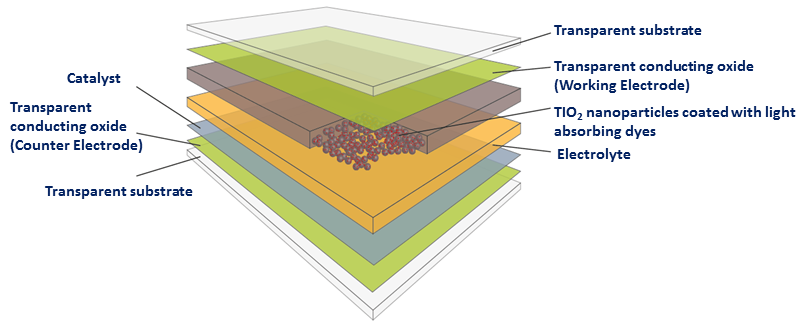
\includegraphics[width=\textwidth]{images/DSCs_struc}
\caption{Structure of a DSC (adapted from \cite{exeger_cell_sand}) }
\label{fig:DSC_struc}
\end{center}
\end{figure}

The most commonly used substrate is glass coated with \ac{FTO}. Attached to the surface of the nano-crystalline particles of Titanium dioxide(\ce{TiO2}) is a mono-layer of the light-sensitive-charge-transfer dye. The dye absorbs photons of incoming light and uses this energy to release free electrons to the \ce{TiO2} layer acting as the \ac{WE} and then onto metal contacts. An electrolyte is filled between the electrodes and helps transfer electrons from the \ac{CE} to the dye particle (which is in an oxidised state due to a loss of electron) to reduce it back to its ground state. The most commonly used redox couple and the one that gives the best cell efficiencies when combined with \ce{TiO2}, is iodide/triiodide (\ce{I-}/\ce{I3-}). The oxidised dye gets electrons from the iodide ions which, in turn, get oxidised to triiodide in the process. The triiodide ions then diffuse to the counter electrode, where they get reduced back to iodide by the electrons returning from the external load. Thus, the cell operation is based on consecutive reduction/oxidation cycles and, in an ideal cell, no chemical substances are permanently transmuted. The most often used counter electrode catalyst for the triiodide/iodide reduction reaction is platinum, though also carbon materials and certain conductive polymers have been successfully employed in this function.\\
\begin{figure}[H]
\begin{center}
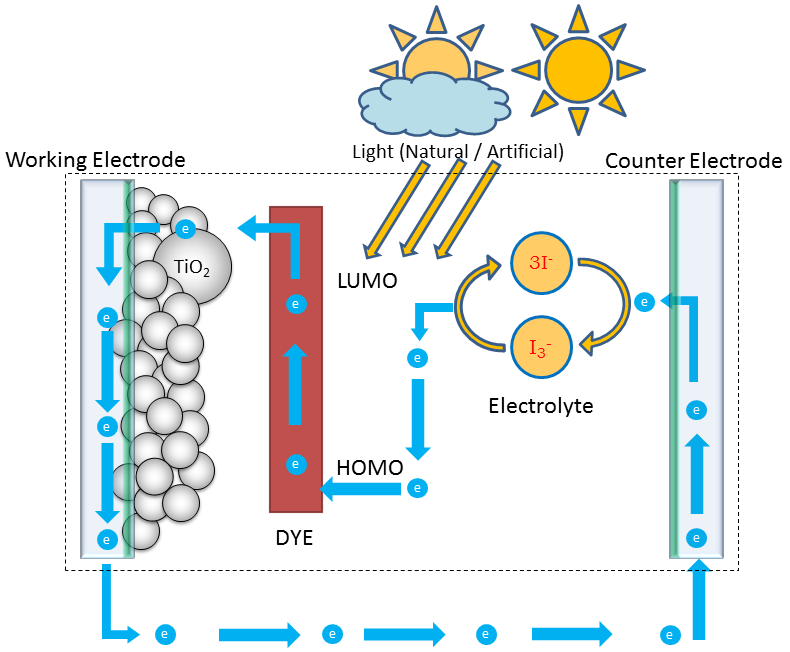
\includegraphics[width=\textwidth]{images/Cell_Cycle}
\caption{ The structure and operating principle of a DSC (adapted from \cite{toivola2010dye,}\cite{gcell_DSSC_cycle})}
\label{fig:Cell_Cycle}
\end{center}
\end{figure}

The amount of current that the cell is able to generate is determined by the energetic distance of the \ac{HOMO} and \ac{LUMO} of the dye, which equals the band gap in inorganic semiconductors. The maximum voltage, on the other hand, is defined as the difference between the redox level of the electrolyte and the Fermi level of the \ce{TiO2}.With iodide/triiodide redox couple, this difference is 0.9 V, though slight variation is caused by the electrolyte composition due to species adsorbed on the \ce{TiO2} surface, which may somewhat alter the Fermi level position. Also, there is always some recombination in the cell which lessens the amount of electrons in the TiO2 film, thus lowering the Fermi level and decreasing the cell voltage. \cite{toivola2010dye}.  This operating principle of \ac{DSCs} is depicted in the Figure ~\ref{fig:Cell_Cycle} on page ~\pageref{fig:Cell_Cycle}. \\


  
  
\subsection{Single diode model}\label{sec:SDM}
The simplest equivalent circuit of a generic solar cell is a Single diode model comprising of a current source in parallel with a diode.A slightly more detailed model includes a shunt resistance of the cell which takes into account the parallel resistive losses representing leakage current across the junction in the cell. This model is sometimes referred to as a single exponential five-parameter model\cite{vignati2012solutions}. The incident photons induces a current in the active area that is proportional to the intensity of the light falling on the cell.

 \begin{figure}[H]
  \begin{center}
  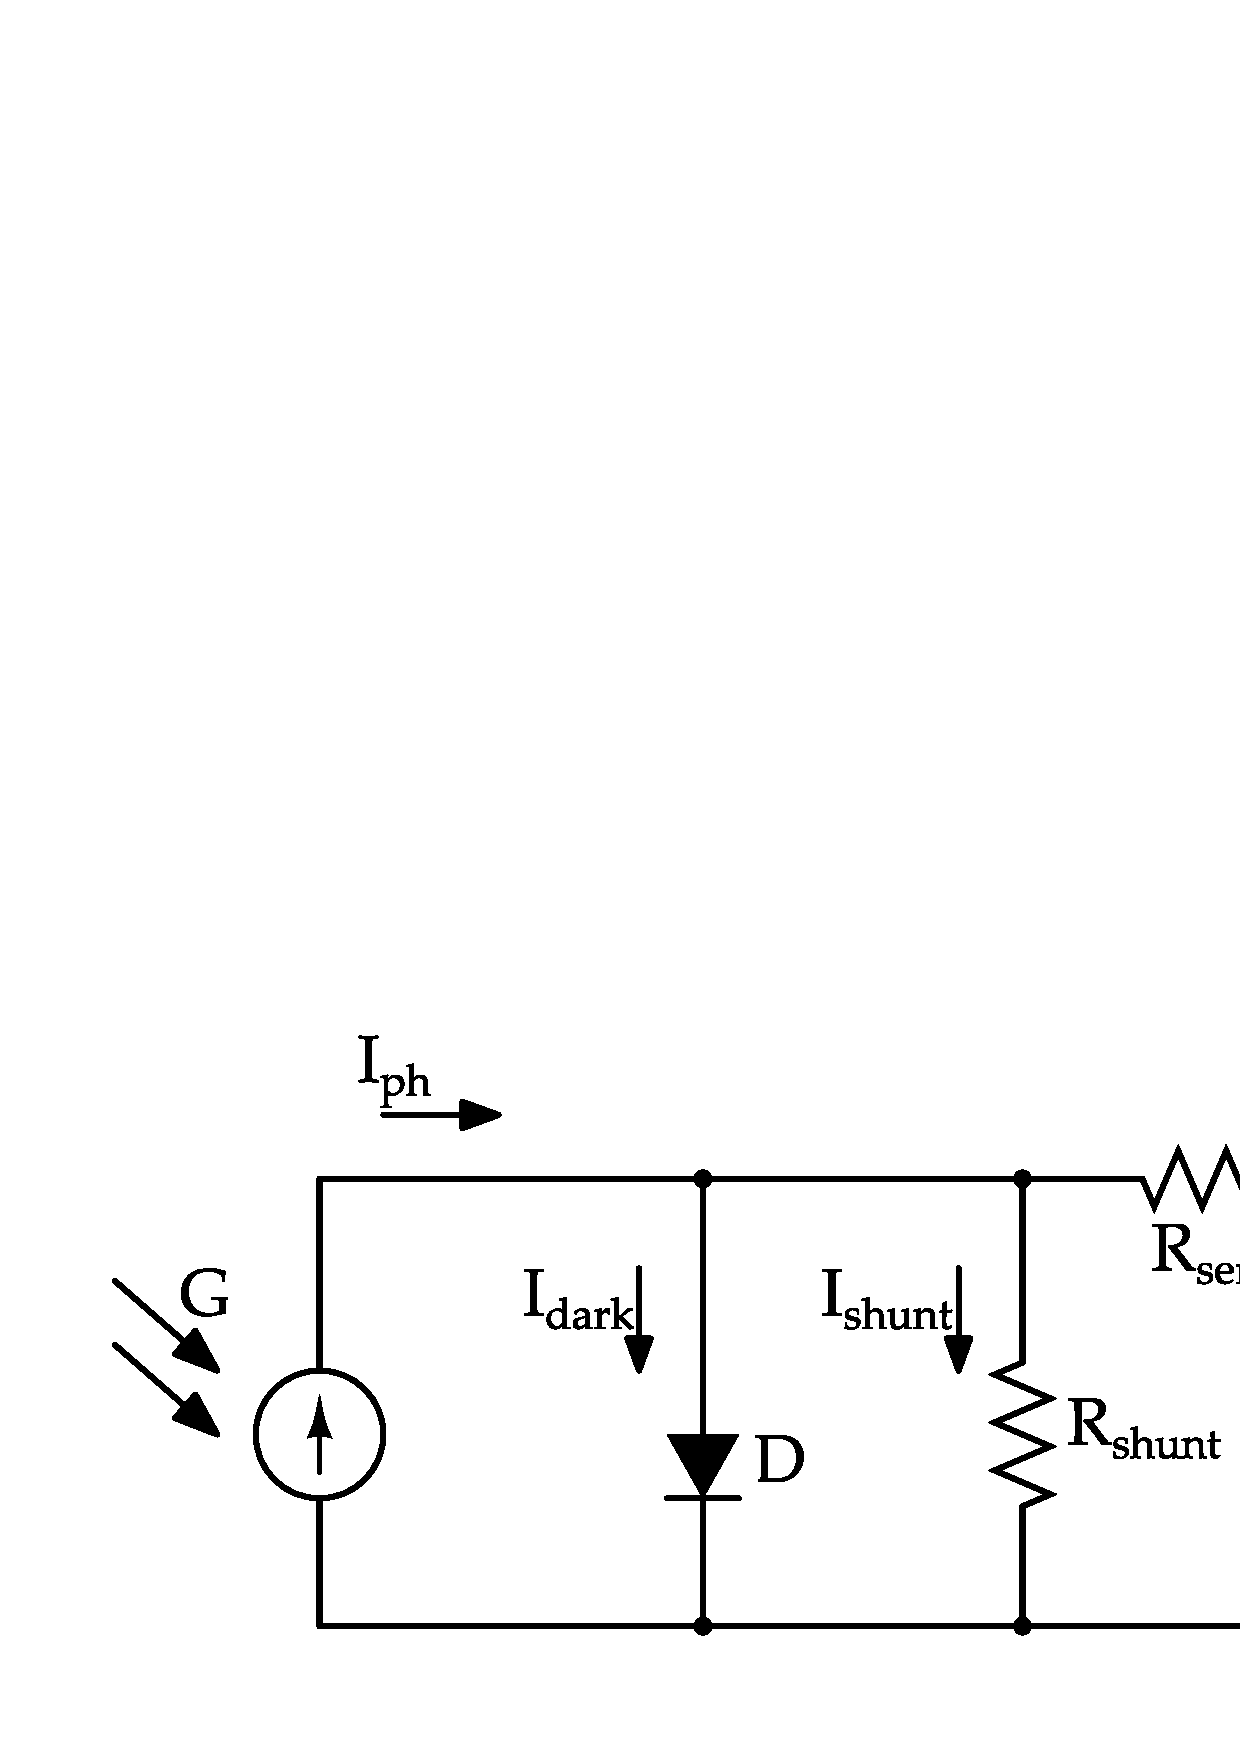
\includegraphics[width=\textwidth]{images/simplified_single_diode_model}
  \caption{ Single diode model for a solar cell }
  \label{fig:EQu_cell}
  \end{center}
  \end{figure}
  
% % % %**Change text**  
The power conversion efficiency of a solar cell is determined from the current versus applied voltage (I-V ) characteristics under illumination. The I-V curve and device efficiency are reported with respect to a standard reference spectral irradiance distribution, the air mass 1.5 global (AM 1.5G) spectrum\cite{wenger2010strategies}. The I-V characteristics of a solar cell are well described by an equivalent electric circuit in Figure ~\ref{fig:EQu_cell} on page ~\pageref{fig:EQu_cell} . Under illumination, a constant photo current (I\textsubscript{ph}) is generated. If a forward voltage bias is applied, a dark diode current (I\textsubscript{dark}) flows in the opposite direction. A shunt resistance (R\textsubscript{shunt}) may arise from charge recombination in the photo-active layer and induce a shunting current(I\textsubscript{shunt}).The series resistance (R\textsubscript{series}) includes the contact resistance at interfaces, the bulk resistance and the sheet resistance of the transparent electrodes. The total measured current then is:
 
 \begin{equation}
 \begin{aligned}
  I = I\textsubscript{ph} - I\textsubscript{dark} - I\textsubscript{shunt} = I\textsubscript{ph} -  I\textsubscript{s} (e^{\frac{eV}{\textit{mk}T}}-1) - \dfrac{V+IR\textsubscript{series}}{R\textsubscript{shunt}}
   \label{eq:equ_current}
   \end{aligned}
   \end{equation}

 where \textbf{I\textsubscript{s}} is the diode saturation current, \textbf{V} is the applied bias voltage, \textbf{\textit{m}} is an ideality factor ( \textit{m} = 1 for an ideal cell), \textbf{\textit{k}} is the Boltzmann constant, and \textbf{T} is the device temperature\cite{wenger2010strategies}. For small forward bias voltages the numerical value of the exponential is very large and 
  the thermal voltage very small, therefore the '-1' in the diode equation can be safely neglected and the forward diode current can be written as\cite{pv_education_org}:
  \begin{equation}
   \begin{aligned}
    I\textsubscript{dark}= I\textsubscript{s} (e^{\frac{eV}{\textit{mk}T}}) 
    \label{eq:equ_current_dark}
    \end{aligned}
   \end{equation}
   
   Substituting the value of I\textsubscript{dark} back in equation ~\ref{eq:equ_current} and neglecting the shunt resistance we can simplify the equation to as below (equation ~\ref{eq:equ_new_cell_current}). This can be schematically depicted as Figure ~\ref{fig:simple_EQu_cell} on page ~\pageref{fig:simple_EQu_cell}. The simplified equation suffices for most modelling applications.
   
    \begin{equation}
    \begin{aligned}
     I = I\textsubscript{ph} - I\textsubscript{dark} - I\textsubscript{shunt} = I\textsubscript{ph} -  I\textsubscript{s} (e^{\frac{eV}{\textit{mk}T}})
      \label{eq:equ_new_cell_current}
      \end{aligned}
      \end{equation}
  
     
 \begin{figure}[H]
   \begin{center}
   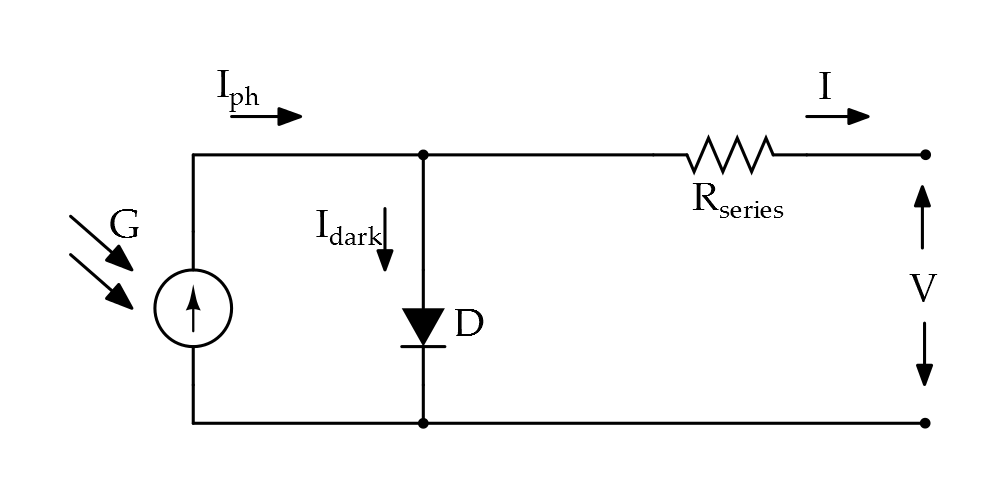
\includegraphics[width=\textwidth]{images/simplified_single_diode_model_simple}
   \caption{ Simplified single diode model for a solar cell }
   \label{fig:simple_EQu_cell}
   \end{center}
   \end{figure}

The maximum-power operating point defines the condition at which the power output (P\textsubscript{\textit{max}} = I\textsubscript{\textit{max}}V\textsubscript{\textit{max}}) of the device is maximal.
The so-called \ac{F.F} is often used to characterise the maximum power ,

\begin{equation}
 \begin{aligned}
  \ac{F.F} = \dfrac{I\textsubscript{\textit{max}}V\textsubscript{\textit{max}}}{I\textsubscript{\textit{sc}}V\textsubscript{\textit{oc}}}
   \label{eq:equ_current_new}
   \end{aligned}
   \end{equation}
   
The accuracy and complexity of the model can be increased by including Temperature dependence of the photo current and diode saturation current; shunt resistance in parallel with the diode and accommodating for variance in the quality factor of the diode either by having a variable parameter or introduction of an additional diode into the circuit as done in the Double Diode Model.


\subsection{Double diode model}\label{sec:DDM}

The single diode equation assumes a constant value for the ideality factor \textit{n}. In reality, the ideality factor is a function of voltage across the device. At high voltages, when the recombination in the device is dominated by the surfaces and the bulk regions, the ideality factor is close to one. However at lower voltages, recombination in the junction dominates and the ideality factor approaches two. The junction recombination is modelled by adding a second diode in parallel with the first and setting the ideality factor typically to two(ideality factor, \textit{n} for D\textsubscript{1} = 1 and D\textsubscript{2} = 2)\cite{pv_education_org}.\\

 \begin{figure}[H]
  \begin{center}
  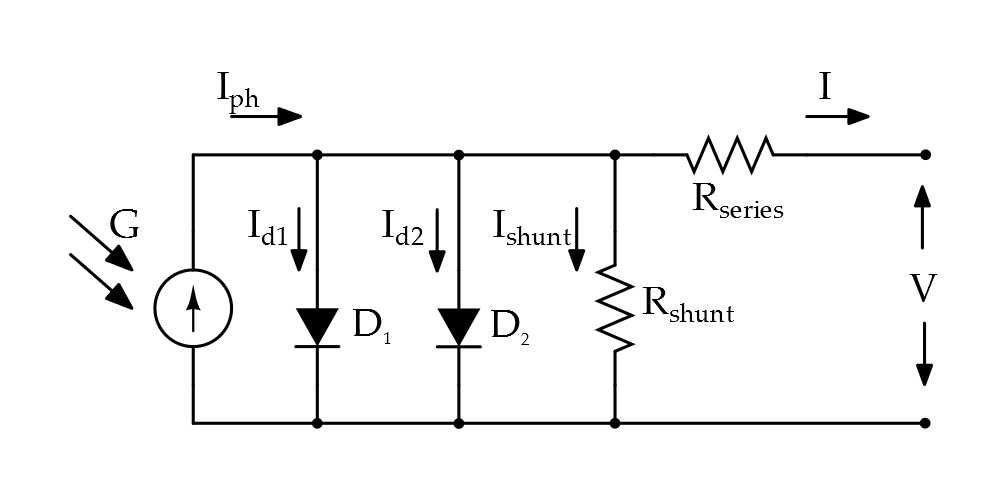
\includegraphics[width=\textwidth]{images/Double_diode_model}
  \caption{ Double diode model for a solar cell (adapted from \cite{pv_education_org}) }
  \label{fig:Double_EQu_cell}
  \end{center}
  \end{figure}
  
The equation of the double diode model under illumination is given by:  

  \begin{equation}
   \begin{aligned}
    I = I\textsubscript{ph} - I\textsubscript{dark} - I\textsubscript{shunt} = I\textsubscript{ph} -  I\textsubscript{s1} (e^{\frac{eV}{\textit{k}T}}-1) - I\textsubscript{s2} (e^{\frac{eV}{2\textit{k}T}}-1)- \dfrac{V+IR\textsubscript{series}}{R\textsubscript{shunt}}
     \label{eq:equ_current_double}
    \end{aligned}
    \end{equation}
  
\subsection{Equivalent DSCs model}\label{sec:eDDM}

It has normally been found that \ac{DSCs} do not conform to the typical I-V curves obtained from transmission line model and ladder circuit\cite{yong2008modeling}. \ac{DSCs} are often modelled with circuits similar to conventional \textit{pn}-junction solar cell ( Section~\ref{sec:SDM} and ~\ref{sec:DDM}), however even these representations fail to correspond to experimentally obtained values.

A standard \ac{DSCs} typically contains three interfaces formed by FTO/TiO\textsubscript{2}, TiO\textsubscript{2}/dye/ electrolyte, and electrolyte/Pt-FTO as depicted in the Figure ~\ref{fig:Cell_Cycle} on page ~\pageref{fig:Cell_Cycle}. The equivalent circuit below (Figure ~\ref{fig:dsc_eq_ckt}) accounts for these interfaces. The interfacial charge transfer at the $TiO_{2}$/ dye/ electrolyte is represented by a rectifying diode(D\textsubscript{1}) and a double-layer capacitance (C\textsubscript{i}). A recombination diode D\textsubscript{2} is employed to denote the interfacial charge recombination losses to both the dye cation and the redox electrolyte. Parallel resistive losses across the cell including leakage current is indicated by R\textsubscript{Shunt}. The photo-generated current I\textsubscript{ph} is in parallel with the diodes and C\textsubscript{i}. An inductive recombination pathway as a result of a charge-transfer current is incorporated into the circuit, consisting of a recombination resistance ( R\textsubscript{rec} in series with the an inductor (L). The charge-transfer resistance and interfacial capacitance at the FTO electrode and electrolyte/Pt-FTO interface are represented by R\textsubscript{E} and C\textsubscript{E}, and R\textsubscript{CE} and C\textsubscript{CE} respectively. The Nernst diffusion of the carrier transport by ions within the electrolyte is denoted by the Warburg impedance (W). A resistance element {R\textsubscript{Series}, designates the bulk and contact resistive losses present in a practical \ac{DSCs}, such as the sheet resistance of the FTO glass, contact resistance etc. The I-V characteristics based on the equivalent circuit model in figure ~\ref{fig:dsc_eq_ckt} is described in equations ~\ref{eq:equ_current_dSC} \cite{yong2008modeling}.
    


 \begin{figure}[H]
  \begin{center}
	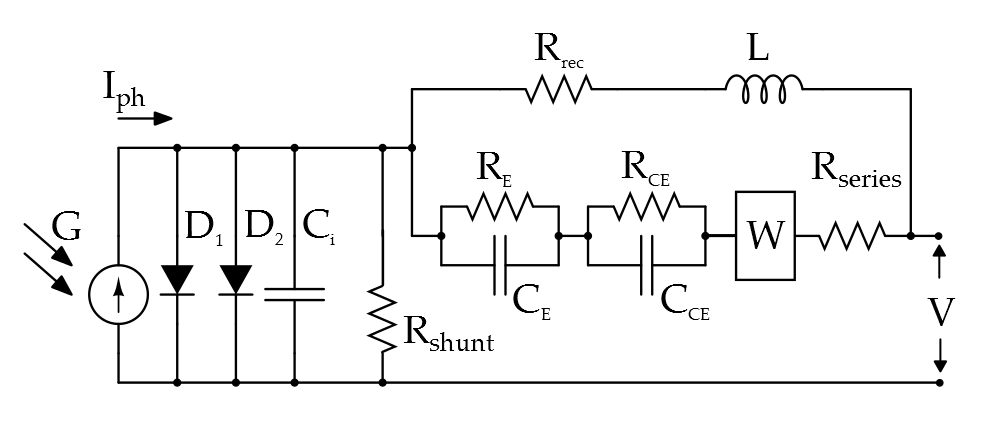
\includegraphics[width=1.0\linewidth]{images/dsc_eq_ckt}
	\caption{Equivalent circuit for DSCs (adapted from \cite{yong2008modeling})  }
	\label{fig:dsc_eq_ckt}
  \end{center}
  \end{figure}

 \begin{equation}
  \begin{aligned}
    I = I\textsubscript{ph} -  I\textsubscript{s1} (e^{\frac{eV}{\textit{mk}T}}-1) - I\textsubscript{s2} (e^{\frac{eV}{2\textit{mk}T}}-1)- (V+IZ)(\textit{j}{\omega}C\textsubscript{i}+\frac{1}{R\textsubscript{Shunt}}) 
     \label{eq:equ_current_dSC}
  \end{aligned}
 \end{equation}
    
 \begin{equation}
  \begin{aligned}
     I\textsubscript{ph} =\int{qF(\lambda)[1-r(\lambda)]IPCE(\lambda)d\lambda} = \int{qF(\lambda)\Phi(\lambda)d\lambda}  
  \end{aligned}
 \end{equation}
 
  \begin{equation}
   \begin{aligned}
     Z={\dfrac{1}{{\frac{1}{(R\textsubscript{rec}+\textit{j}{\omega}L)}}+{\frac{1}{Z\textsubscript{S}}}}} 
   \end{aligned}
  \end{equation}
  
 \begin{equation}
   \begin{aligned}
    Z\textsubscript{S}={\dfrac{1}{{\textit{j}{\omega}C\textsubscript{E}}+{\frac{1}{R\textsubscript{E}}}}}+{\dfrac{1}{{\textit{j}{\omega}C\textsubscript{CE}}+{\frac{1}{R\textsubscript{CE}}}}}+W+R\textsubscript{S}
   \end{aligned}
  \end{equation}
  
   \begin{equation}
     \begin{aligned}
     W = \sigma{\omega^{-1/2}}(1-\textit{j})
     \end{aligned}
    \end{equation}
    
Where T is the absolute temperature, $\omega$ is the angular frequency, $\sigma$ is the Warburg coefficient, $F(\lambda)$ and  $IPCE(\lambda)$ are the incident photon flux density and the incident photon-to-current conversion efficiency at wavelength $\lambda$ respectively, $r(\lambda)$ is the incident light losses due to the light absorption and reflection by the FTO glass, and $\Phi(\lambda)$ is the quantum yield \cite{yong2008modeling}.\newline

  




% %**Pictures and text about losses in the light absorption in the cell **

% %**talk ABOUT STABILITY OF dcs with change in temperature **

\section{Maximum Power Point Tracking(MPPT)}


Despite all the advantages presented by the generation of energy through the use of solar cells the efficiency of energy conversion is currently low (the best commercial solar module is only 21.5\% efficient) and the initial cost for its implementation is still considered high. Thus it becomes pertinent to use various techniques to extract the maximum power from these cells, in order to achieve maximum efficiency in operation. It should be noted that there is only one maximum power point (MPP) for a given panel, and this varies according to climatic and irradiation conditions\cite{eltawil2013mppt}.

To overcome this problem, several methods for extracting the maximum power have been proposed and many comparative studies have been published in literature  \cite{chu2009robust}, \cite{clark2006power}, \cite{eltawil2013mppt}, \cite{esram2007comparison}, \cite{faranda2008energy}, \cite{houssamo2013experimental}, \cite{ngan2011study} and \cite{reza2013classification}. 

\subsection{Perturb and Observe (PnO) Method } \label{sec:pno_sec}


    \begin{figure}[H]
       \begin{center}
       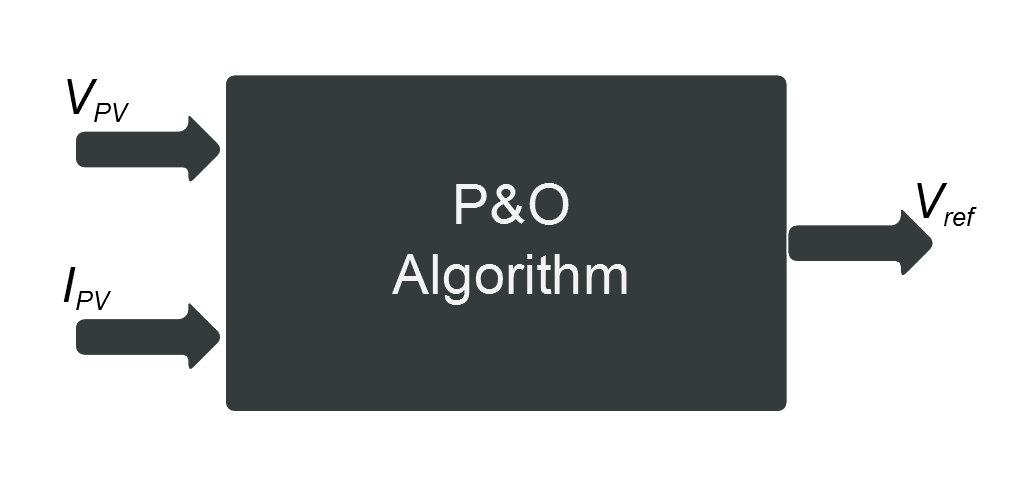
\includegraphics[width=0.4\textwidth]{images/PnO_block}
       \caption{ Black box model for the Perturb and Observe Algorithm }
       \label{fig:PnO_block}
       \end{center}
       \end{figure}
       
  The \ac{PnO} Method is most widely used in \ac{MPPT} because of  its simple structure and it requires only few parameters. Figure ~\ref{fig:PnO_flow}  shows the flow chart of \ac{PnO} method. It perturbs the PV array's terminal voltage periodically and then it compares the PV output power with that of the previous cycle of perturbation. When PV power and PV voltage increase at the same time and vice versa, a perturbation step size, ${\Delta}$D will be added to the duty cycle, D to generate the next cycle of   perturbation in order to force the operating point moving towards the \ac{MPP}. When PV power increases and PV voltage decreases and vice versa, the perturbation step will be subtracted for the next cycle of perturbation. This process will be carried on continuously until \ac{MPP} is reached. However, the system will oscillate around the \ac{MPP} throughout this process, and this will result in loss of energy. These oscillations can be minimised by reducing the perturbation step size but it significantly slows down the \ac{MPP} tracking system also leading to loss of energy \cite{ngan2011study}. \ac{PnO} is also not suitable when the light intensity changes rapidly. \\ %** explain why not suitable**
  
  \begin{figure}[H]
    \begin{center}
    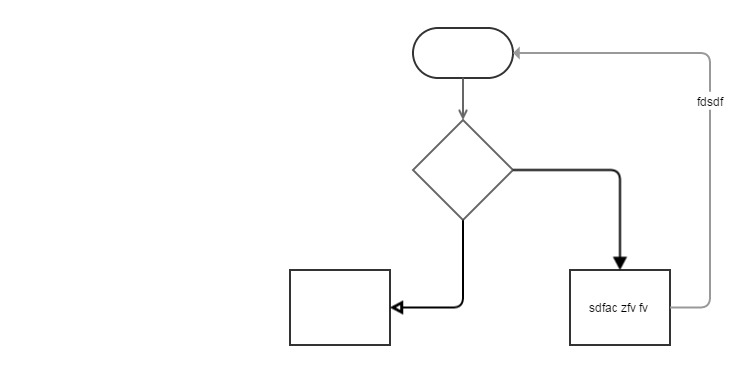
\includegraphics[width=\textwidth]{images/pno_flow}
    \caption{Flow chart for the Perturb and Observe Method }
    \label{fig:PnO_flow}
    \end{center}
    \end{figure}
  
  \subsection{Incremental Conductance Method (ICM) } \label{sec:icm_sec}
  
  \begin{figure}[H]
         \begin{center}
         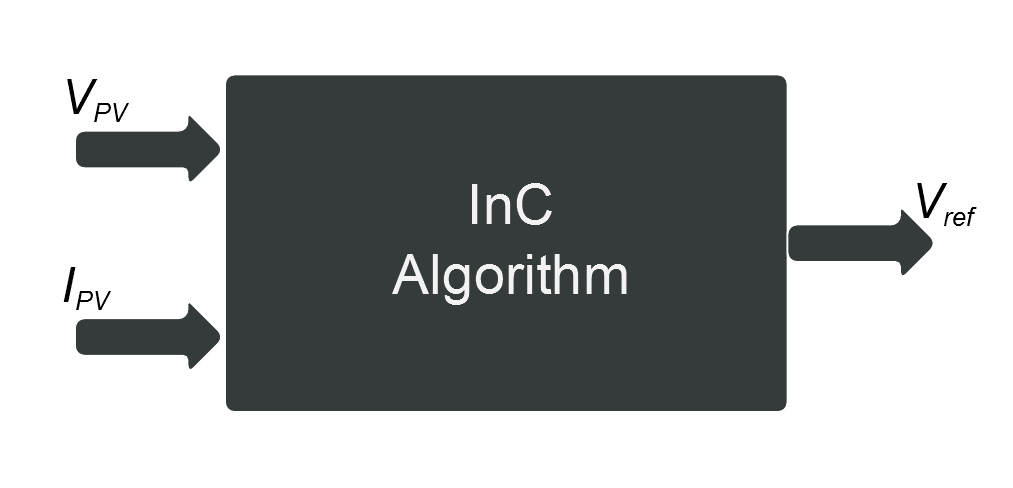
\includegraphics[width=0.4\textwidth]{images/inC_block}
         \caption{ Black box model for the Incremental Conductance Algorithm }
         \label{fig:inC_block}
    \end{center}
  \end{figure}
  
  The  solar array terminal  voltage  can  be  adjusted relative to the MPP voltage by measuring the incremental and instantaneous  array  conductance (dI/dV and I/V, respectively). The algorithm is based on the fact that at the \ac{MPP}, the derivative of the cell's power is zero. Although  the  incremental  conductance method offers good performance under rapidly changing atmospheric  conditions, four  sensors  are  required to perform the computations. The  drawback is that sensor devices require  more  conversion  time  thus  resulting in a large amount of power loss \cite{gomathy2012design}. In addition to the above drawback, the \ac{ICM} suffers the same limitations as \ac{PnO} method namely, for rapid tracking larger step sized must be utilised which results in the oscillation around the \ac{MPP}. \\
  
   \begin{figure}[H]
      \begin{center}
      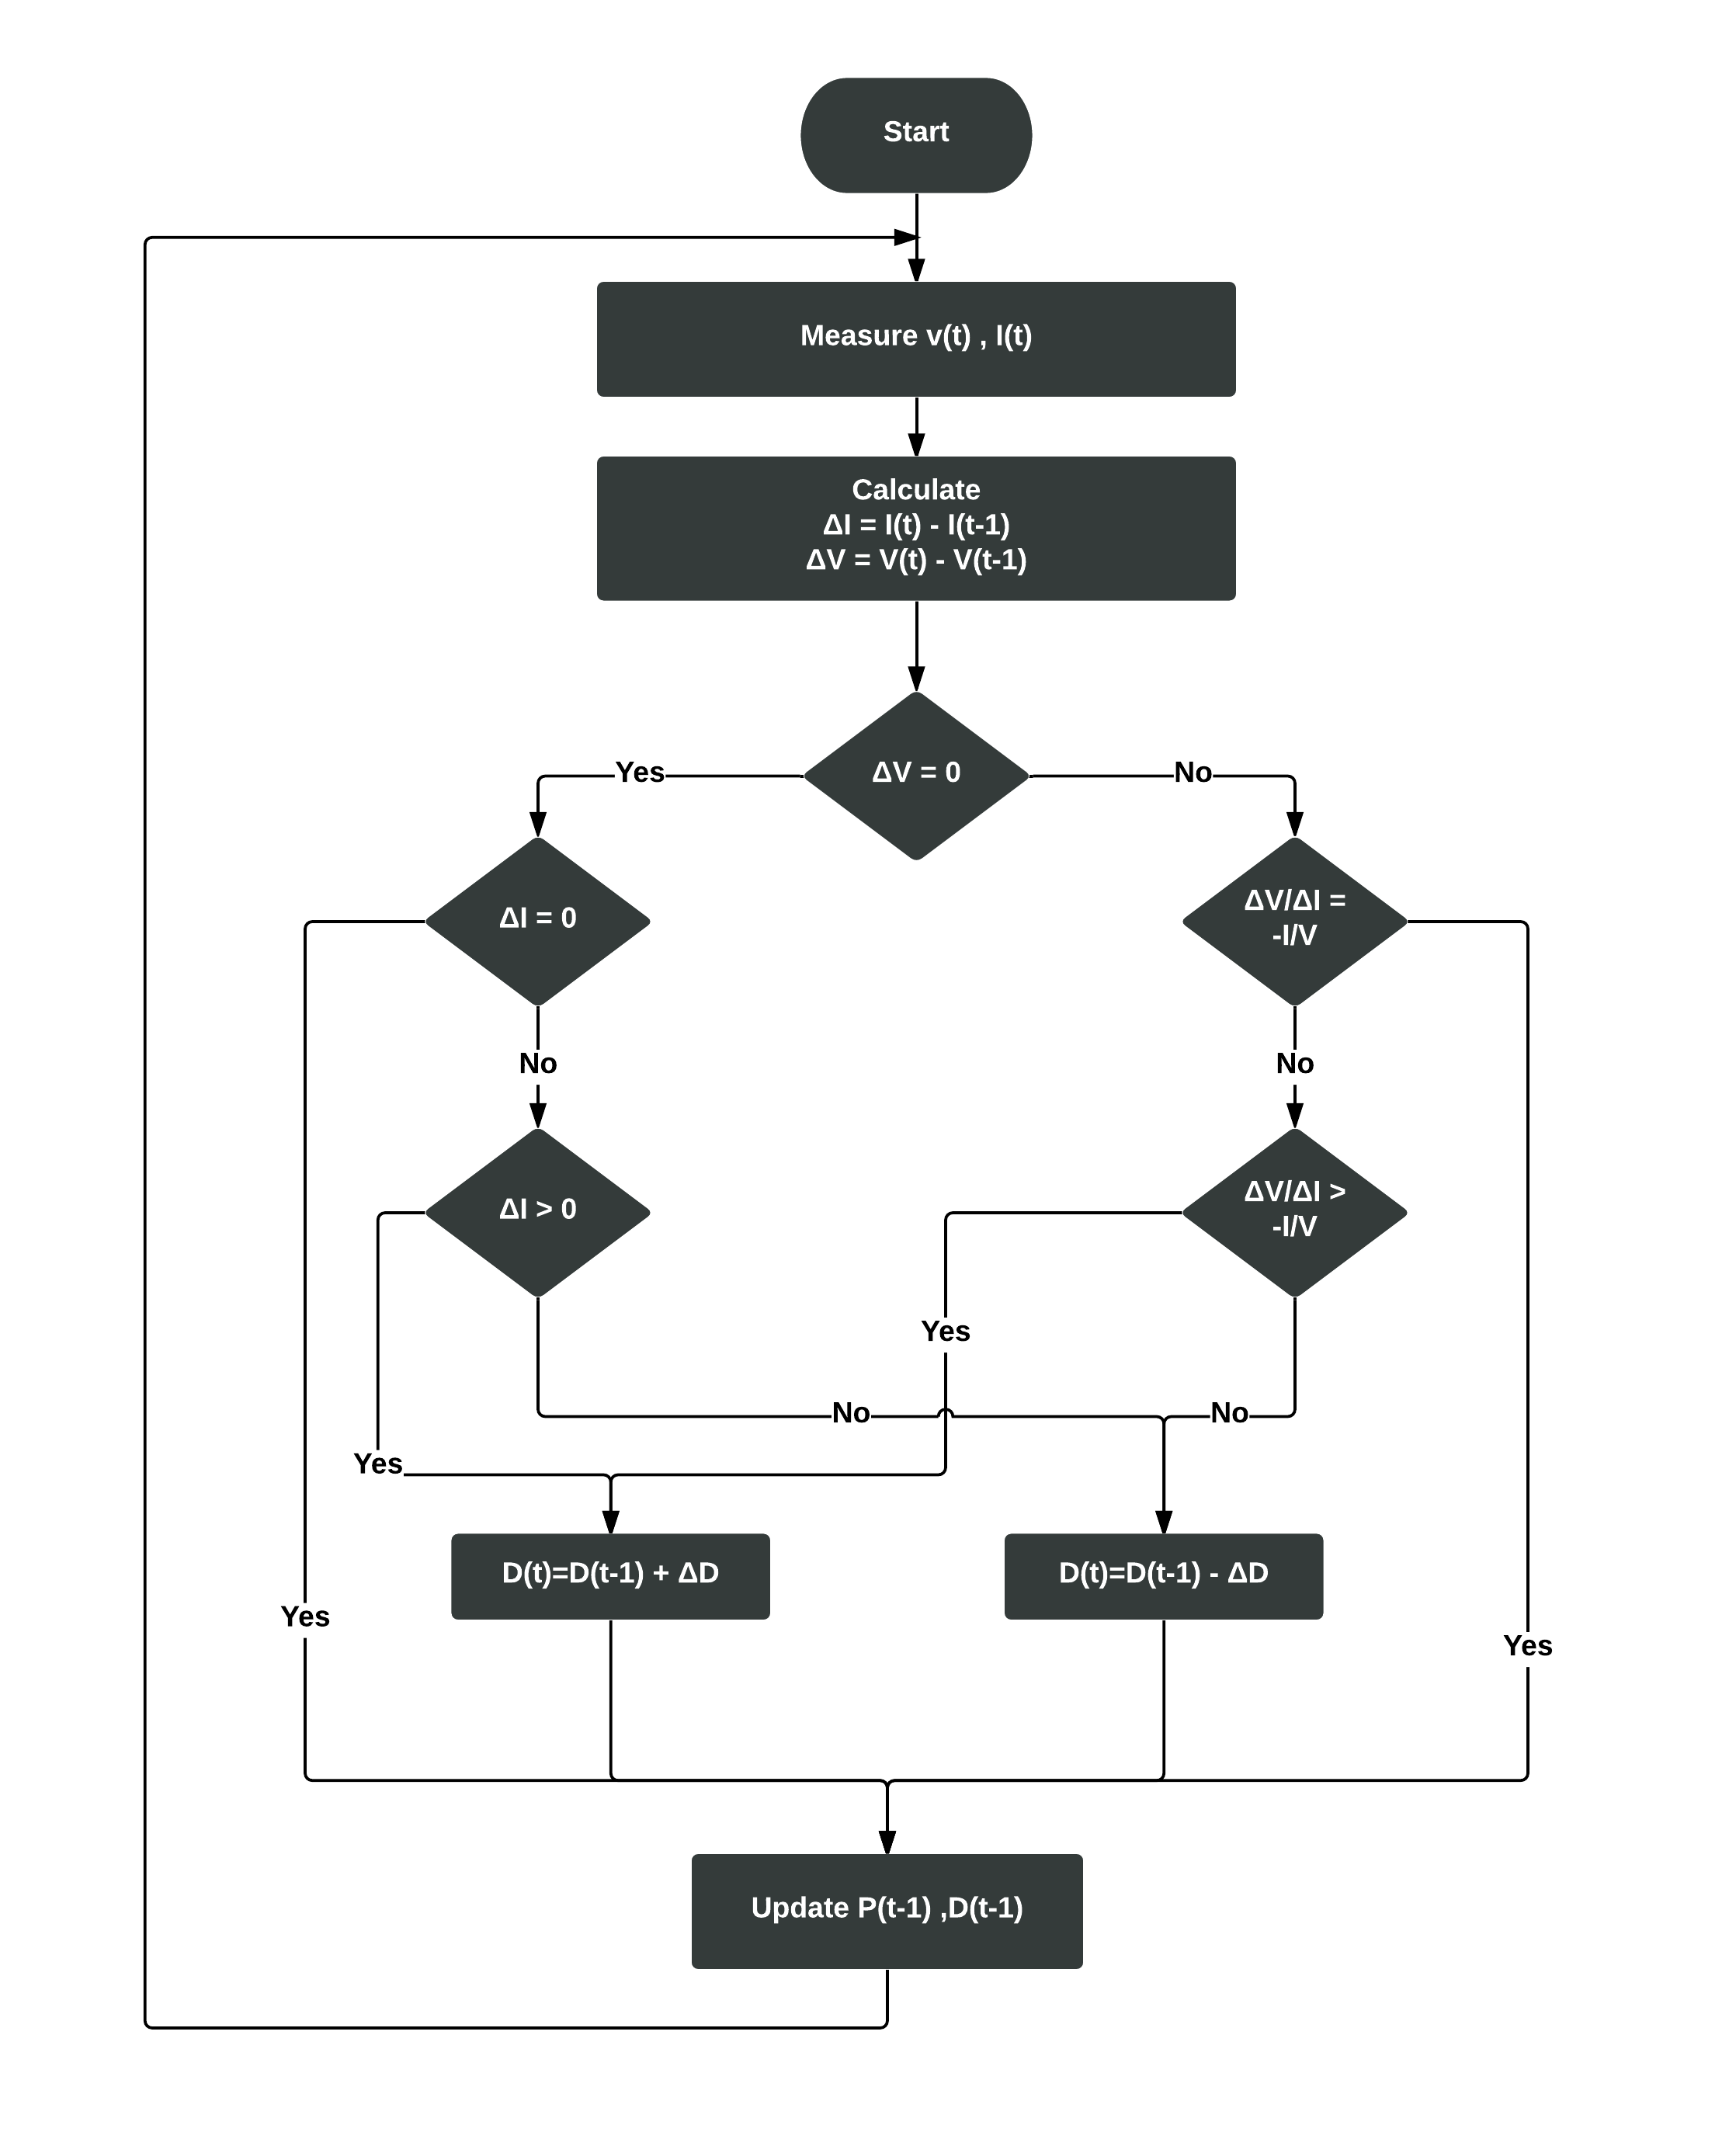
\includegraphics[width=\textwidth]{images/INc_flow}
      \caption{ Flow chart for the Incremental Conductance Method}
      \label{fig:inCflow}
      \end{center}
      \end{figure}
      
  \subsection{Fractional Open Circuit Voltage (FOCV) Method  } \label{sec:focv_sec}
  
   \begin{figure}[H]
           \begin{center}
           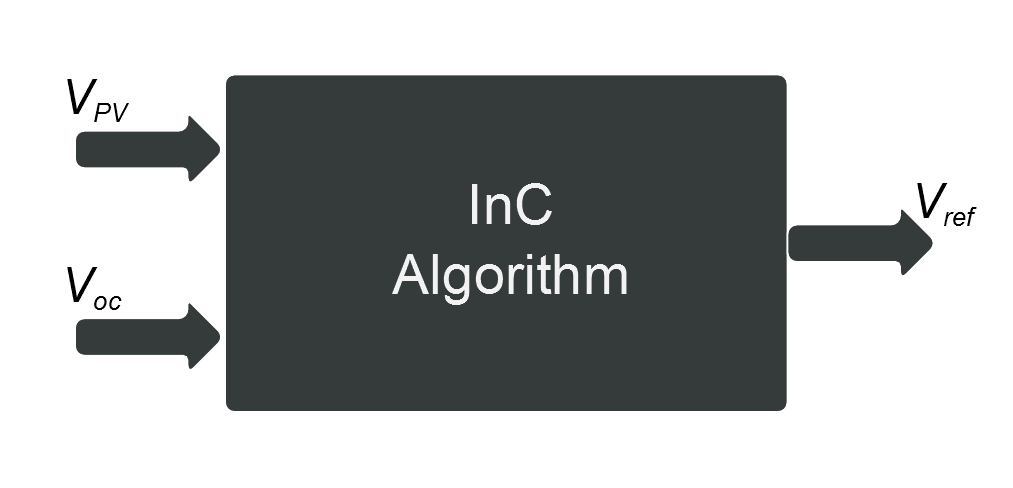
\includegraphics[width=0.4\textwidth]{images/Frac_block}
           \caption{ Black box model for the Incremental Conductance Algorithm }
           \label{fig:Frac_block}
      \end{center}
    \end{figure}
  This is a method based on the linear relationship between output voltage of the PV array at the \ac{MPP}, V\textsubscript{MPP} and the PV array's open circuit voltage, V\textsubscript{OC} in under varying temperature and solar irradiance. \\
  
  \begin{equation}
    \begin{aligned}
  V\textsubscript{MPP}\approx k\textsubscript{i}V\textsubscript{OC}
  \label{eq:equ_fracoc}
  \end{aligned}
  \end{equation}
  
  Constant value of k\textsubscript{i} is dependent on the characteristics of PV array. Generally, it has to be computed empirically in order to determine the V\textsubscript{MPP} and V\textsubscript{OC} for varied temperatures and solar irradiances. The value of k\textsubscript{i} ranges from 0.73 to 0.80  for most PV modules over a temperature range of 0 to 60$^\circ$C.Figure ~\ref{fig:focflow} describes the operation of a \ac{FOCV}, the PV array is temporarily isolated from \ac{MPPT},then the open circuit voltage, V\textsubscript{OC} is measured periodically by shutting down the power converter momentarily. The \ac{MPPT} calculates V\textsubscript{MPP} from the pre-set value of k\textsubscript{i} and the calculated value of V\textsubscript{OC}. Then, the array's voltage is varied until V\textsubscript{MPP} is  reached . The shut-down of power converter periodically will incur temporary loss of power which in turn leads to a situation where power extracted will not be the maxima. Since it is an approximation, the PV array will never reach the \ac{MPP}. Even though this technique is very easy and cheap for implementation; due to the fact true \ac{MPP} is never reached, there is always a loss in power during operation\cite{ngan2011study}.
  
  \begin{figure}[H]
        \begin{center}
        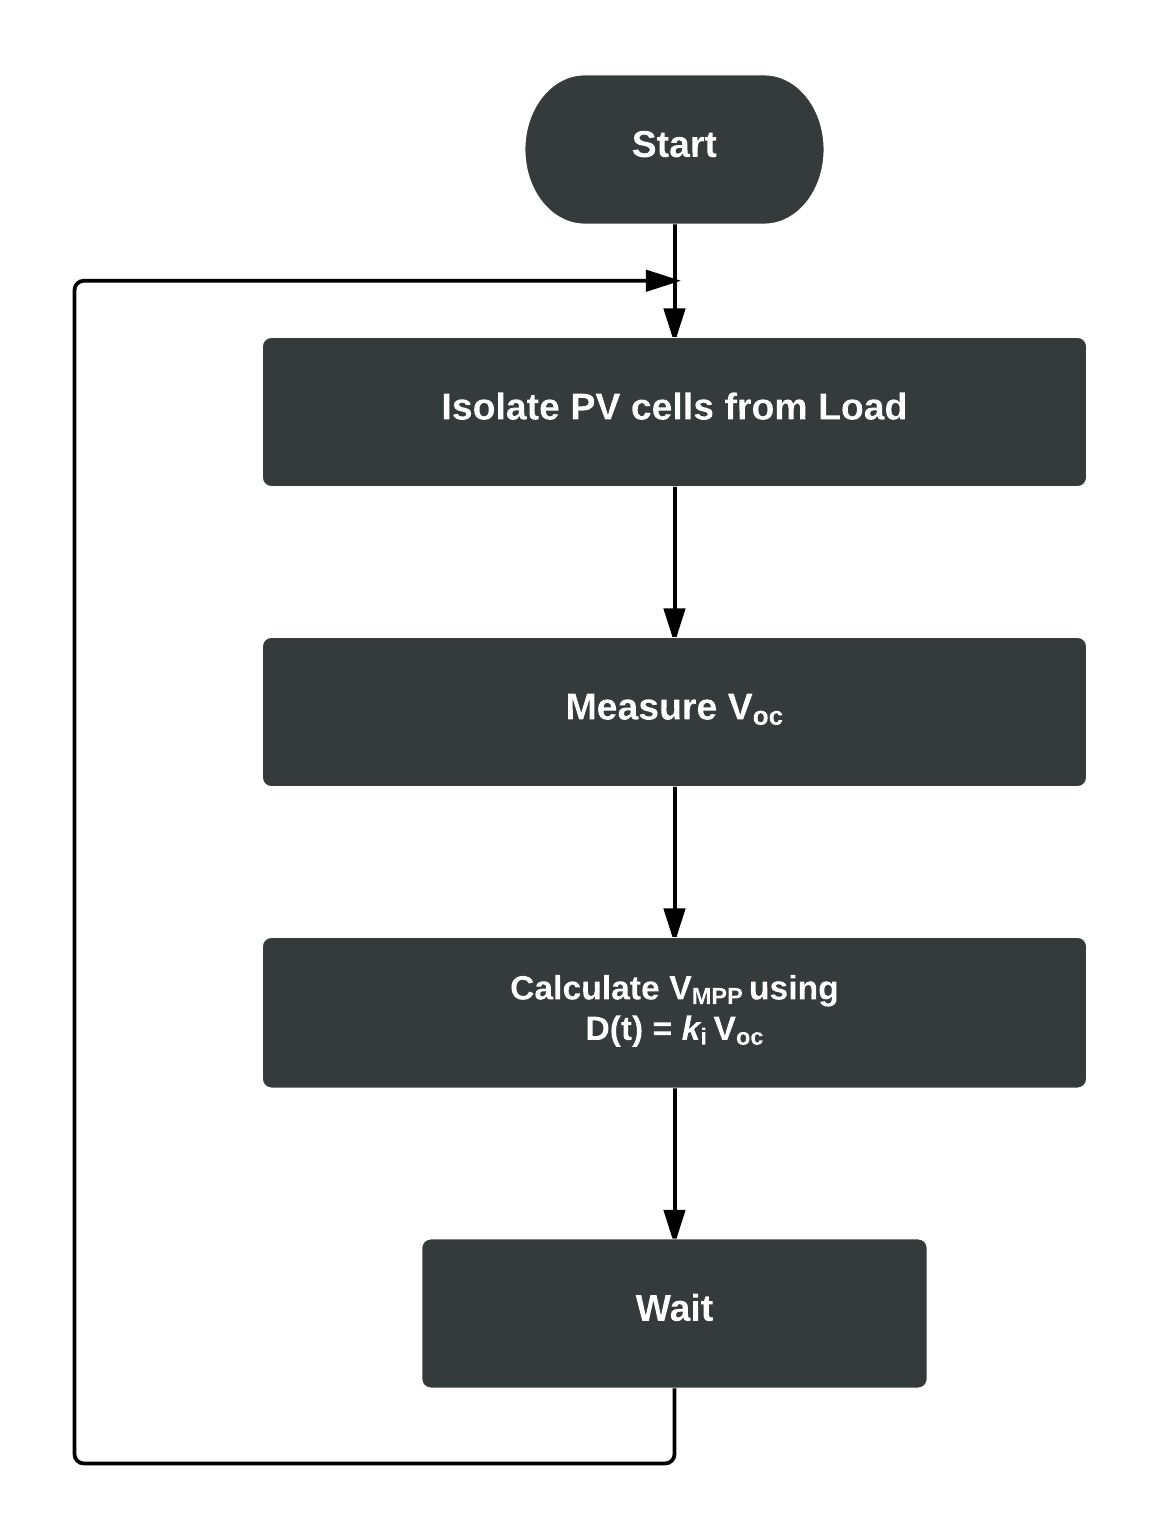
\includegraphics[width=0.5\textwidth]{images/Vopen_circuit_Flow}       %Frac_Flow}
        \caption{ Flow chart for the Fractional Open Circuit Voltage Method (adapted from \cite{reza2013classification})}
        \label{fig:focflow}
        \end{center}
        \end{figure}
  
\subsection{Other algorithms}
  \begin{itemize}
  \item {\bf Fixed duty cycle}: The fixed duty cycle represents the simplest of the methods and it does not require any feedback, where the load impedance is adjusted only once for the maximum power point and it is not adjusted again.
  \item {\bf Pilot cell}: In the pilot cell MPPT algorithm, the constant voltage or current method is used, but the open-circuit voltage or short-circuit current measurements are made on a small solar cell, called a pilot cell, that has the same characteristics as the cells in the larger solar array. The pilot cell measurements can be used by the MPPT to operate the main solar array at its MPP, eliminating the loss of PV power during the V\textsubscript{OC} or I\textsubscript{sc} measurement
  \item {\bf Fractional short-circuit current }: Under varying atmospheric conditions, I\textsubscript{MPP} is approximately linearly related to the I\textsubscript{SC} of the PV array. \newline
    \begin{equation}
      \begin{aligned}
    I\textsubscript{MPP} \approx k\textsubscript{j}I\textsubscript{SC}
    \label{eq:equ_fracoc_cur}
    \end{aligned}
    \end{equation}
   \item {\bf Fuzzy logic controller} (FLC):They have the advantages of working with imprecise inputs, it does not need an accurate mathematical model and it can handle non-linearity as well \cite{messai2011maximum}.However their effectiveness depends a lot on the presence of an expert knowledge; conversely, in the absence of such knowledge, their design is usually slow and not optimised. 
  \end{itemize} 
  







\section{Machine Learning }
This section discusses about Search optimization in order to lock on the  V\textsubscript{MP} and I\textsubscript{MP} as efficiently as possible.\\

Much like Embedded systems, Machine Learning encompasses various disciplines, predominantly Computer science but also statistics, Mathematics, Finance etc. \cite{marsland2011machine}; with applications ranging from predicting emergency-room wait-times \cite{connelly2004discrete} to High Frequency Stock-trading. Simply put, Machine learning is about algorithms that build models which adapt or modify their response in order to get closer to the correct output. These models are automatically created and they constantly evolve based on input vectors, as opposed to having a hard coded decision tree.\\

If the input vectors provided to the algorithm in its training set are 'labelled' , then this kind of learning is called \textbf{Supervised learning}. Where correct or expected responses are provided based on this the algorithm is able to generalise the out put for all possible outputs. In the other end of the spectrum is \textbf{Unsupervised learning} in which the algorithm is left to find hidden structures in a set of data that doesn't have any labels or that all have the same label. In our application we know the input is V\textsubscript{OC} and what the expected Output (V\textsubscript{MPP})is supposed to be. This constitutes as  labelling and hence classified as Supervised learning.
 
\subsection{Regression Modelling }

We use regression analysis when we want to predict one variable from another. The most basic form of regression is called simple regression, where one independent variable and one dependent variable exists and where linear trend is to be predicted. In regression, we attempt to determine the magnitude of the relationship between a set of independent variables and the dependent variable. Independent variable(X), also called the predictor variable, influences the Dependent variable(Y),sometimes called the response variable  \cite{lenarreg2006}.\\

A regression model is a formal way of stating:
\begin{itemize}
\item The tendency of the response variable(Y) to vary with the predictor variable(X).
\item A scattering of points around some statistical relationship.
\end {itemize}

Equation for a line can be written as:

\begin{equation}
\begin{aligned}
  y= mx + b 
\label{eq:Line_equ}
\end{aligned}
\end{equation}

The linear regression model(for observation i = 1, . . . , N) can we written as:

\begin{equation}
\begin{aligned}
  Y\textsubscript{i}= \beta\textsubscript{0}+\beta\textsubscript{1}X\textsubscript{i} +\epsilon\textsubscript{i}
\label{eq:Line_equ_exp}
\end{aligned}
\end{equation}

\begin{itemize}
\item $\beta\textsubscript{0}$ is the mean of the population when X is zero -the Y intercept.
\item $\beta\textsubscript{1}$ is the slope of the line, the amount of increase in Y brought about by a unit increase $(X^{'}= X + 1)$ in X.
\item \textbf{$\epsilon\textsubscript{i}$} is the random error, specific to each observation.
\item the goal is to find $\beta\textsubscript{0}$ and $\beta\textsubscript{1}$ such that $\sum\limits_{i=1}^n \epsilon\textsubscript{i}^2$ is minimised.
\end {itemize}
A large number of methods and procedures have been developed to estimate the parameters of a model, the simplest being :\\

\begin{equation}
	\begin{aligned}
		\beta\textsubscript{1}= \dfrac{\sum (X\textsubscript{i} - \bar{X})(Y\textsubscript{i} - \bar{Y})}{\sum (X\textsubscript{i} - \bar{X})^2} 
	\label{eq:B1_calculus}
	\end{aligned}
\end{equation}

\begin{equation}
	\begin{aligned}
		\beta\textsubscript{0}= \bar{Y}-\beta\textsubscript{1}\bar{X} 
	\label{eq:B0_calculus}
	\end{aligned}
\end{equation}

\begin{figure}[H]
  \begin{center}
  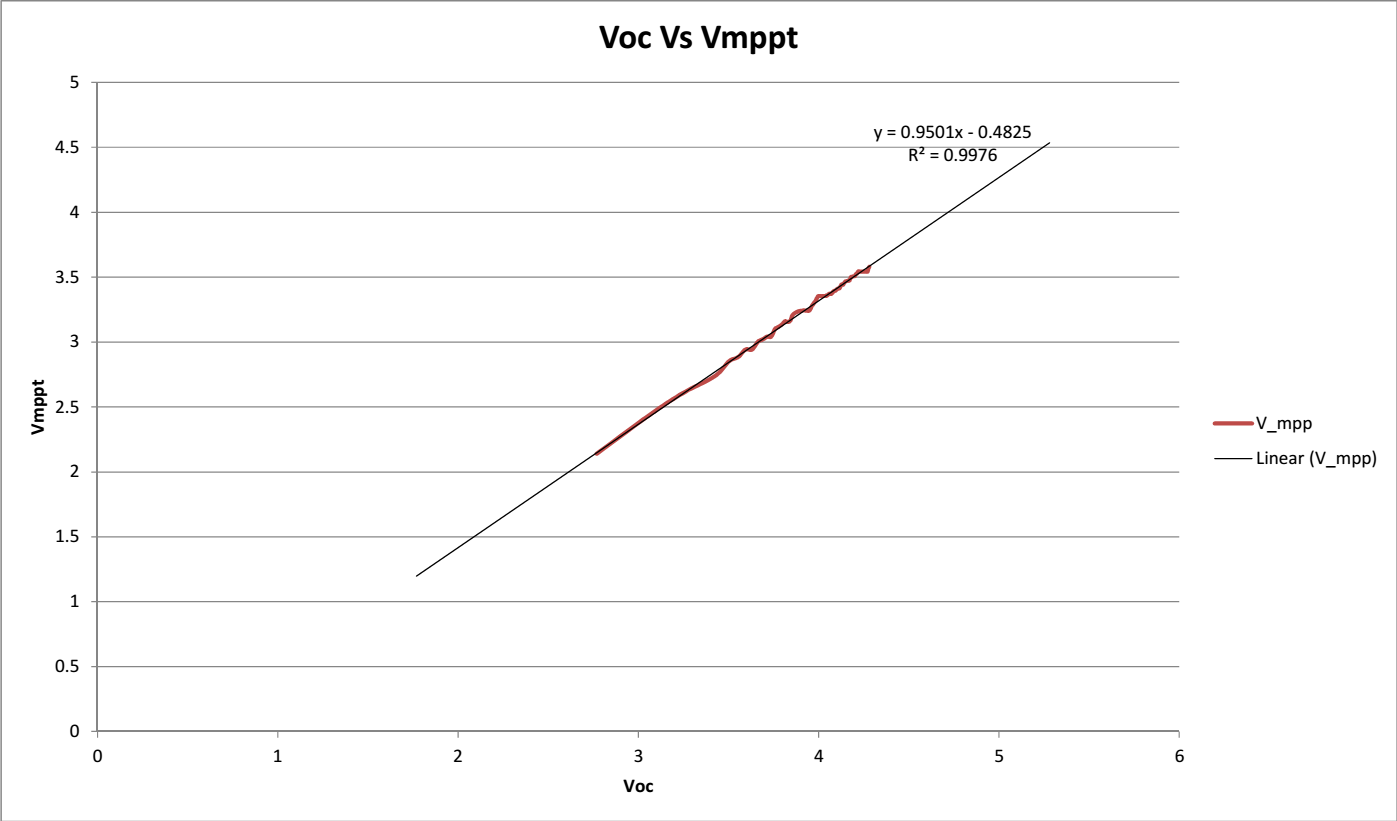
\includegraphics[width=\textwidth]{images/Reg_line}
  \caption{ Example for Linear regression }
  \label{fig:linear_regression}
  \end{center}
  \end{figure}


In Figure ~\ref{fig:linear_regression} the points in red represent $V_{MPP}$ for a given $V_{OC}$. It is clear from the graph that the relationship between $V_{MPP}$ and $V_{OC}$ is linear, this is also supported in various literature (\cite{reza2013classification},\cite{esram2007comparison},etc.) and forms the basis of \ac{FOCV} method. The trend line in black (obtained via Regression Modelling) tells us about the slope of the line ($\beta\textsubscript{1}$) and the Y intercept. It also provides the $R^{2}$ value of the fit equal to 0.9976, indicating the goodness of fit. $R^{2}$ is a measure of how close the regression line is to the data points, with $R^{2} = 1 $ signifying that the model/regression-line perfectly fits the data \cite{Jim_R_squared}.


\subsection{Pattern search}


Finding the maxima or minima ( collectively known as extrema) of a first order single variable function can easily be found by equating the derivative of this function to zero. However finding the derivative of certain functions is not always easy or possible. In such conditions, various search techniques are used to find the maxima or minima  in a uni-modal ( a uni-modal function contains only one minimum or maximum on the specified interval) continuous function over an interval without using derivatives \cite{seiler1989numerical}. \ac{GSSA} is one such search method. The algorithm derives its name from the Golden ratio (0.61803...)\\

Two numbers are said to be in the Golden ratio if their ratio is same as the ratio of their sum to the larger of the two quantities. Assuming $\beta > \alpha$ then this can be expressed as\cite{Gill81MurrayWright}:\\

\begin{equation}
	\begin{aligned}
		\dfrac{\alpha+\beta}{\beta}=\dfrac{\beta}{\alpha}=\phi
		\label{eq:golden_ratio1}
	\end{aligned}
\end{equation}

where ${\phi}$ is the Golden ratio whose value is given by:\\

\begin{equation}
	\begin{aligned}
		 \phi=\dfrac{\sqrt{5}-1}{2}= 0.61803398874989......
		\label{eq:golden_ratio}
	\end{aligned}
\end{equation}
 
 Assuming \textit{f(x)} to be an uni-modal function in the intervals between  \textit{a} and \textit{b}. It is very important for the extrema exists within the range to prevent misleading results. The maxima is represented by $\textit{f}(P_{\textit{max}})$ such that $a\leq P_{\textit{max}} \leq b $.
 \begin{itemize}
 
 \item Points $P_{1} \& P_{2}$ are chosen such that they satisfy:
 
\begin{equation}
	\begin{aligned}
		 P_{1}=a+(1-\phi)(b-a)
		\label{eq:golden_ratio_p1}
	\end{aligned}
\end{equation}

\begin{equation}
	\begin{aligned}
		 P_{2}=a+\phi(b-a)
		\label{eq:golden_ratio_p2}
	\end{aligned}
\end{equation}


	\item $\textit{f}(a),\textit{f}(P_{1}),\textit{f}(P_{2})$ and $\textit{f}(b)$ is computed.
	\item If $\textit{f}(P_{1}) > \textit{f}(P_{2})$ then the outer bound is discarded and replaced by $ P_{2} $ and $ P_{2}$ replaced $ P_{1}$; a new $ P_{1}$ is calculated using equation ~\ref{eq:golden_ratio_p1}.
	\item Else the lower bound is cast-off to be replaced with $ P_{1}$ and $ P_{1}$ is swapped with $ P_{2}$; with $ P_{2}$ found afresh using equation ~\ref{eq:golden_ratio_p2}.
	\item New values of either $\textit{f}(P_{1})$ or $\textit{f}(P_{2})$ are found out depending on the branch taken.
	\item  The process repeated over and over again only stopping when either the iteration count has run out or if the lower and upper bounds are close enough to be acceptably small. 
\end{itemize}

 
\begin{figure}[H]
  \begin{center}
  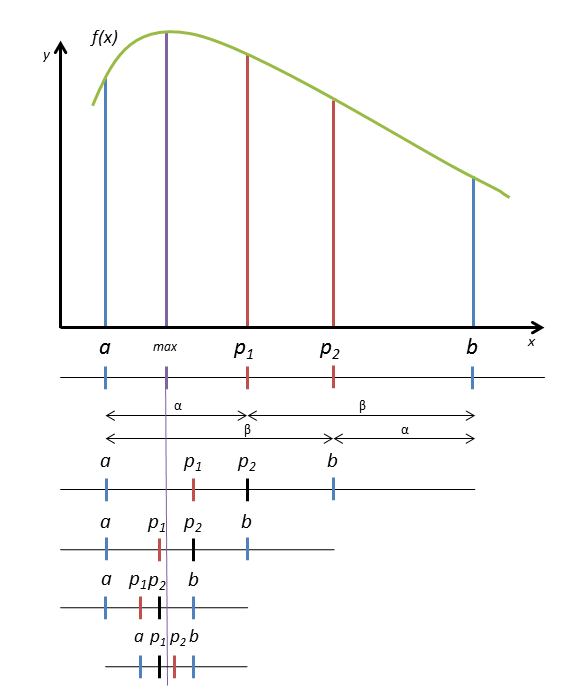
\includegraphics[width=0.92\textwidth]{images/Golden_search_curve}
  \caption{ Golden Section search algorithm }
  \label{fig:Golden_search_curve}
  \end{center}
  \end{figure}
  
The advantage of using \ac{GSSA} over other search methods is that the extrema is found in the least number of steps and every iteration requires only one additional data point. Thereby greatly reducing the complexity of the algorithm and hence the computation power and/or time required to lock-in onto the extrema.

\begin{itemize}
	 \item The blue points represent extremes of the successive
	 \item Red points  are the newly evaluated values
	 \item Black points are the already evaluated values.
 \end{itemize}


 
\begin{figure}[H]
  \begin{center}
  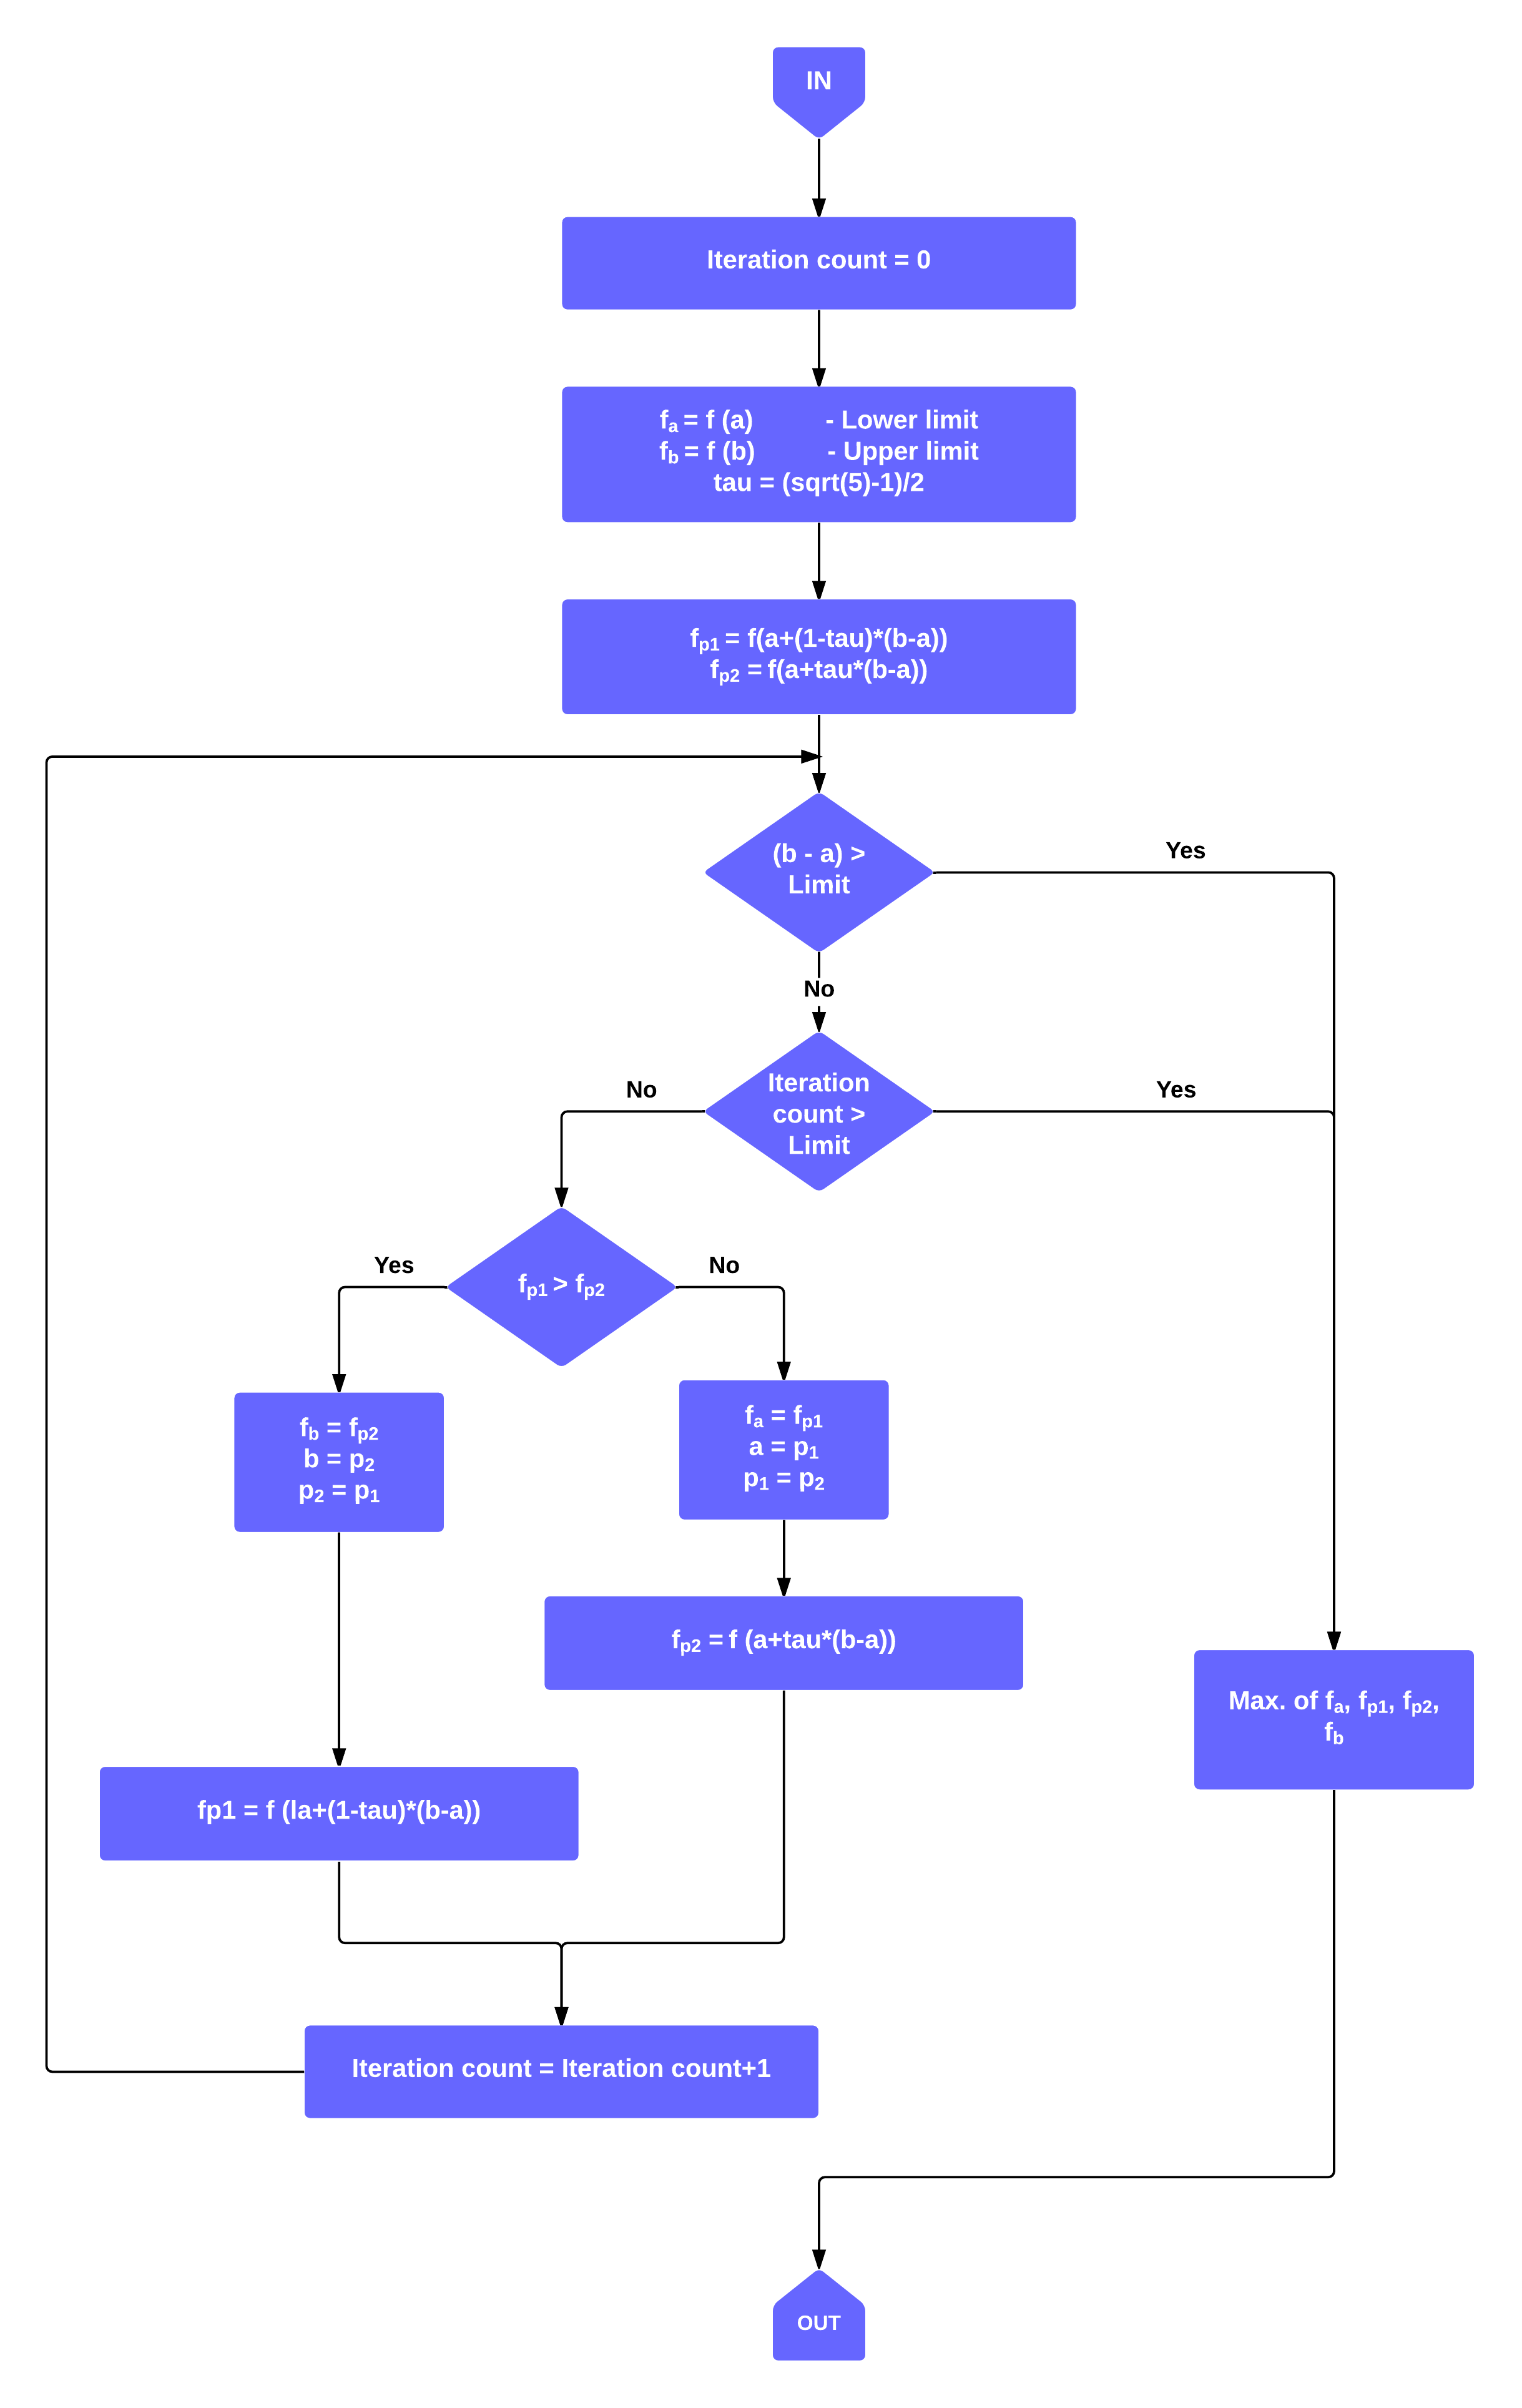
\includegraphics[width=\textwidth]{images/Golden_Search}
  \caption{ Golden Section search algorithm (modified from \cite{van1970fitting})}
  \label{fig:Golden_search}
  \end{center}
  \end{figure}
  
 

	\chapter{Design and Implementation}
\begin{quote} 
\it This chapter covers the implementation details of the concept, the algorithms. All the simulations were first carried out in MATLAB{\textregistered} and Simulink{\textregistered}, testing and verifying.The section also introduces the proposed hybrid algorithm.
\end{quote}
%\right 

\section{Cell Characterisation}
In this section, Model of two types of cells (\ac{a-Si} and \ac{DSCs}) is discussed.There are several Models that have been analysed in literature which are usually variations of the Single Diode model or the Double Diode model (discussed in section \ref{sec:SDM},\ref{sec:DDM} and \ref{sec:eDDM}).
 
\subsection{Test Setup}

 In the pursuance of creating a working solar cell model and to validate the algorithm several measurements would need to be performed. The Test-rig consisted of a blacked out enclosure to suppress interference from ambient light. The Test-rig or Light-box is fitted with an array of evenly spaced White-\ac{LED}s to provide uniform illumination on the Test subject. The \ac{LED}-array are calibrated and temperature controlled so as to provide white light with a known spectra. A high precision Lux Meter(\textit{GOSSEN Mavolux 5032B}) is used to measure the  intensity of the light, as perceived by the human eye. The \textit{GOSSEN} serves as a reference for Lux measurement throughout the project. The Light chamber is also routinely calibrated against a reference cell to factor-in the variations and degradation of the \ac{LED}s. The intensity of light is varied using a High-Voltage power source. A pictorial representation of the above description can be seen is figure ~\ref{fig:test setup} on page ~\pageref{fig:test setup}. \\



 \begin{figure}[H]
	  \begin{center}
		  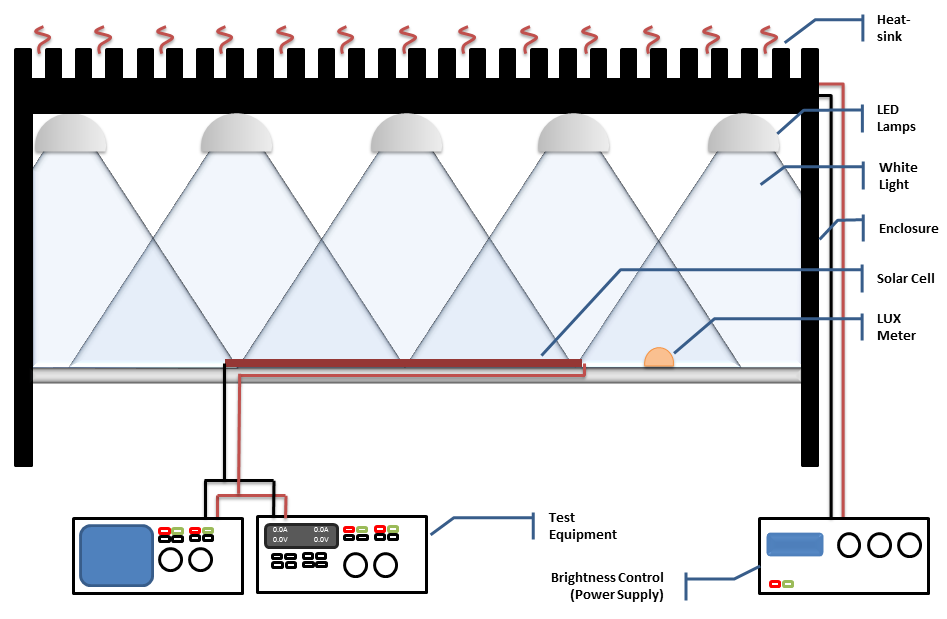
\includegraphics[width=\textwidth]{images/Light_Box}
		  \caption{Test Setup }
		  \label{fig:test setup}
	  \end{center}
  \end{figure}
  

Electrical models for solar cells are frequently found in literature \cite{vignati2012solutions} and \cite{yong2008modeling} among others -discussed in section \ref{sec:SDM} to \ref{sec:eDDM}.However \ac{DSCs} come in may different flavours:- dissimilar electrolytes \& electrodes; additional layers and junctions. Added to this fact, due to the near impossibility of accurately measuring the multitude of variables of a unknown cell, for this research work, a model was constructed by placing a the test cell under a battery of varied illuminations (0 Lux - 5050 Lux) shown in figure ~\ref{fig:Voltagevlux}. Which resulted in a surface that closely resembles the cell's operation under real world conditions. Particular attention was paid to low light conditions which is to be expected for indoor illuminations ( < 2000 Lux).As \ac{DSCs} display are very stable output across temperature ranges found indoor \cite{lee2010high}, the above model was made independent of temperature variations.

 \begin{figure}[H]
  \begin{center}
	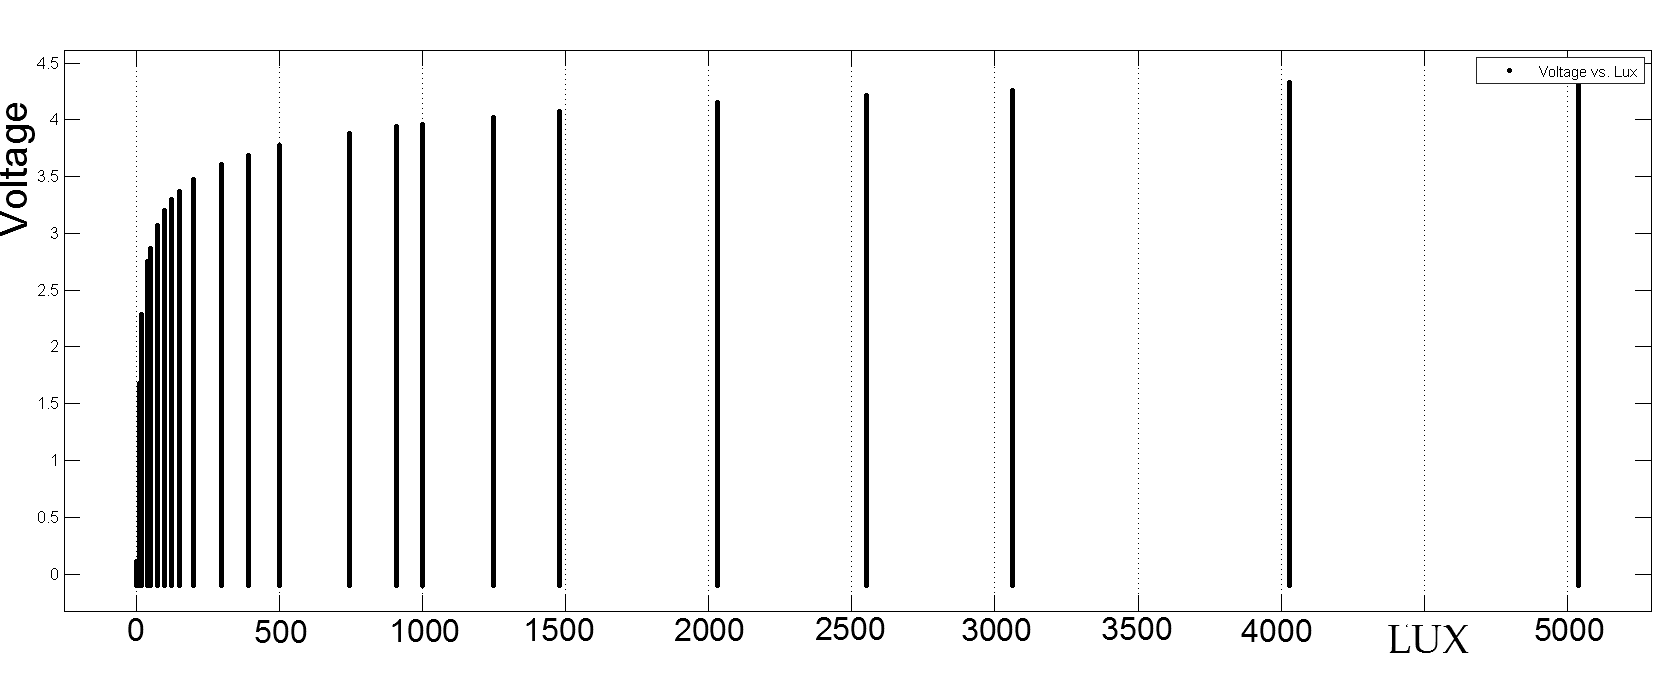
\includegraphics[width=0.9\linewidth]{images/Voltagevlux}
	\caption{spread of measured illumination vs Voltage  }
	\label{fig:Voltagevlux}
  \end{center}
 \end{figure}
 The Cell-under-test is connected to a \ac{SMU}. \ac{SMU}s have flexibility in their outputs, to be classified as having four-quadrant outputs, it must be able to source power as well as sink power. Sourcing power refers to providing the stimulus for a circuit, and sinking power refers to dissipating power that is being applied by an external active component such as a battery, a charged capacitor, or another power source \cite{NI_SMU} - a solar cell in our case.
 \begin{figure}[H]
	  \begin{center}
		  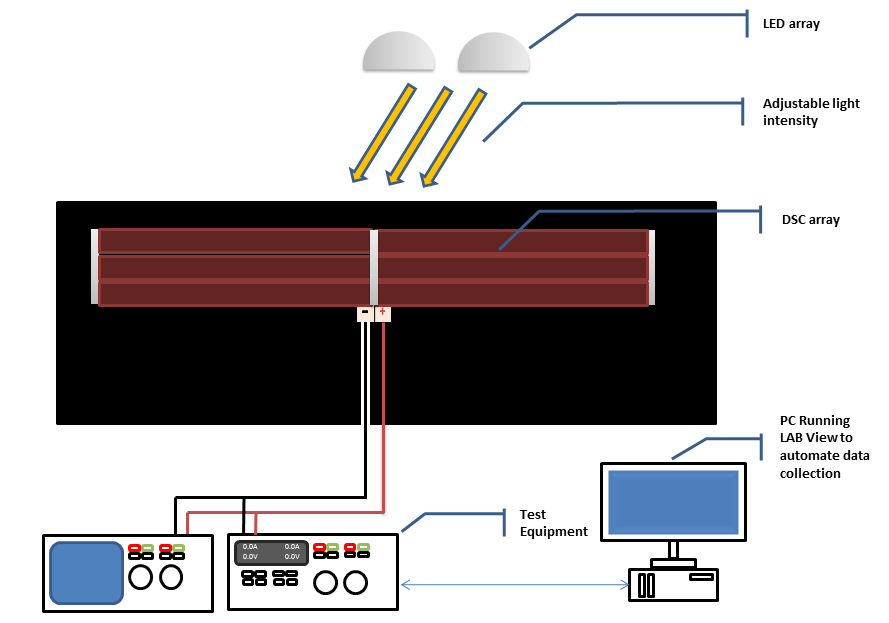
\includegraphics[width=\textwidth]{images/Cell_under_test}
		  \caption{Cell Characterisation }
		  \label{fig:Cell_U_test}
	  \end{center}
 \end{figure}
 As the Sink potential is increased in tiny increments, starting from  0 V to V\textsubscript{OC} and beyond, the cell is forced to operate at the Sink Voltage resulting in the I-V graph depicted in figure ~\ref{fig:2500luxIV} on page ~\pageref{fig:2500luxIV}. When the above is repeated for several different light intensities we get a three-dimensional surface shown in figure ~\ref{fig:luxIV100_2500} on page ~\pageref{fig:luxIV100_2500}.Note that, V\textsubscript{OC} is the maximum voltage available from a cell this occurs when the cell produces zero Current (when the graph intersects the \textit{x}-axis).\\
 
  \begin{figure}[H]
	  \begin{center}
		  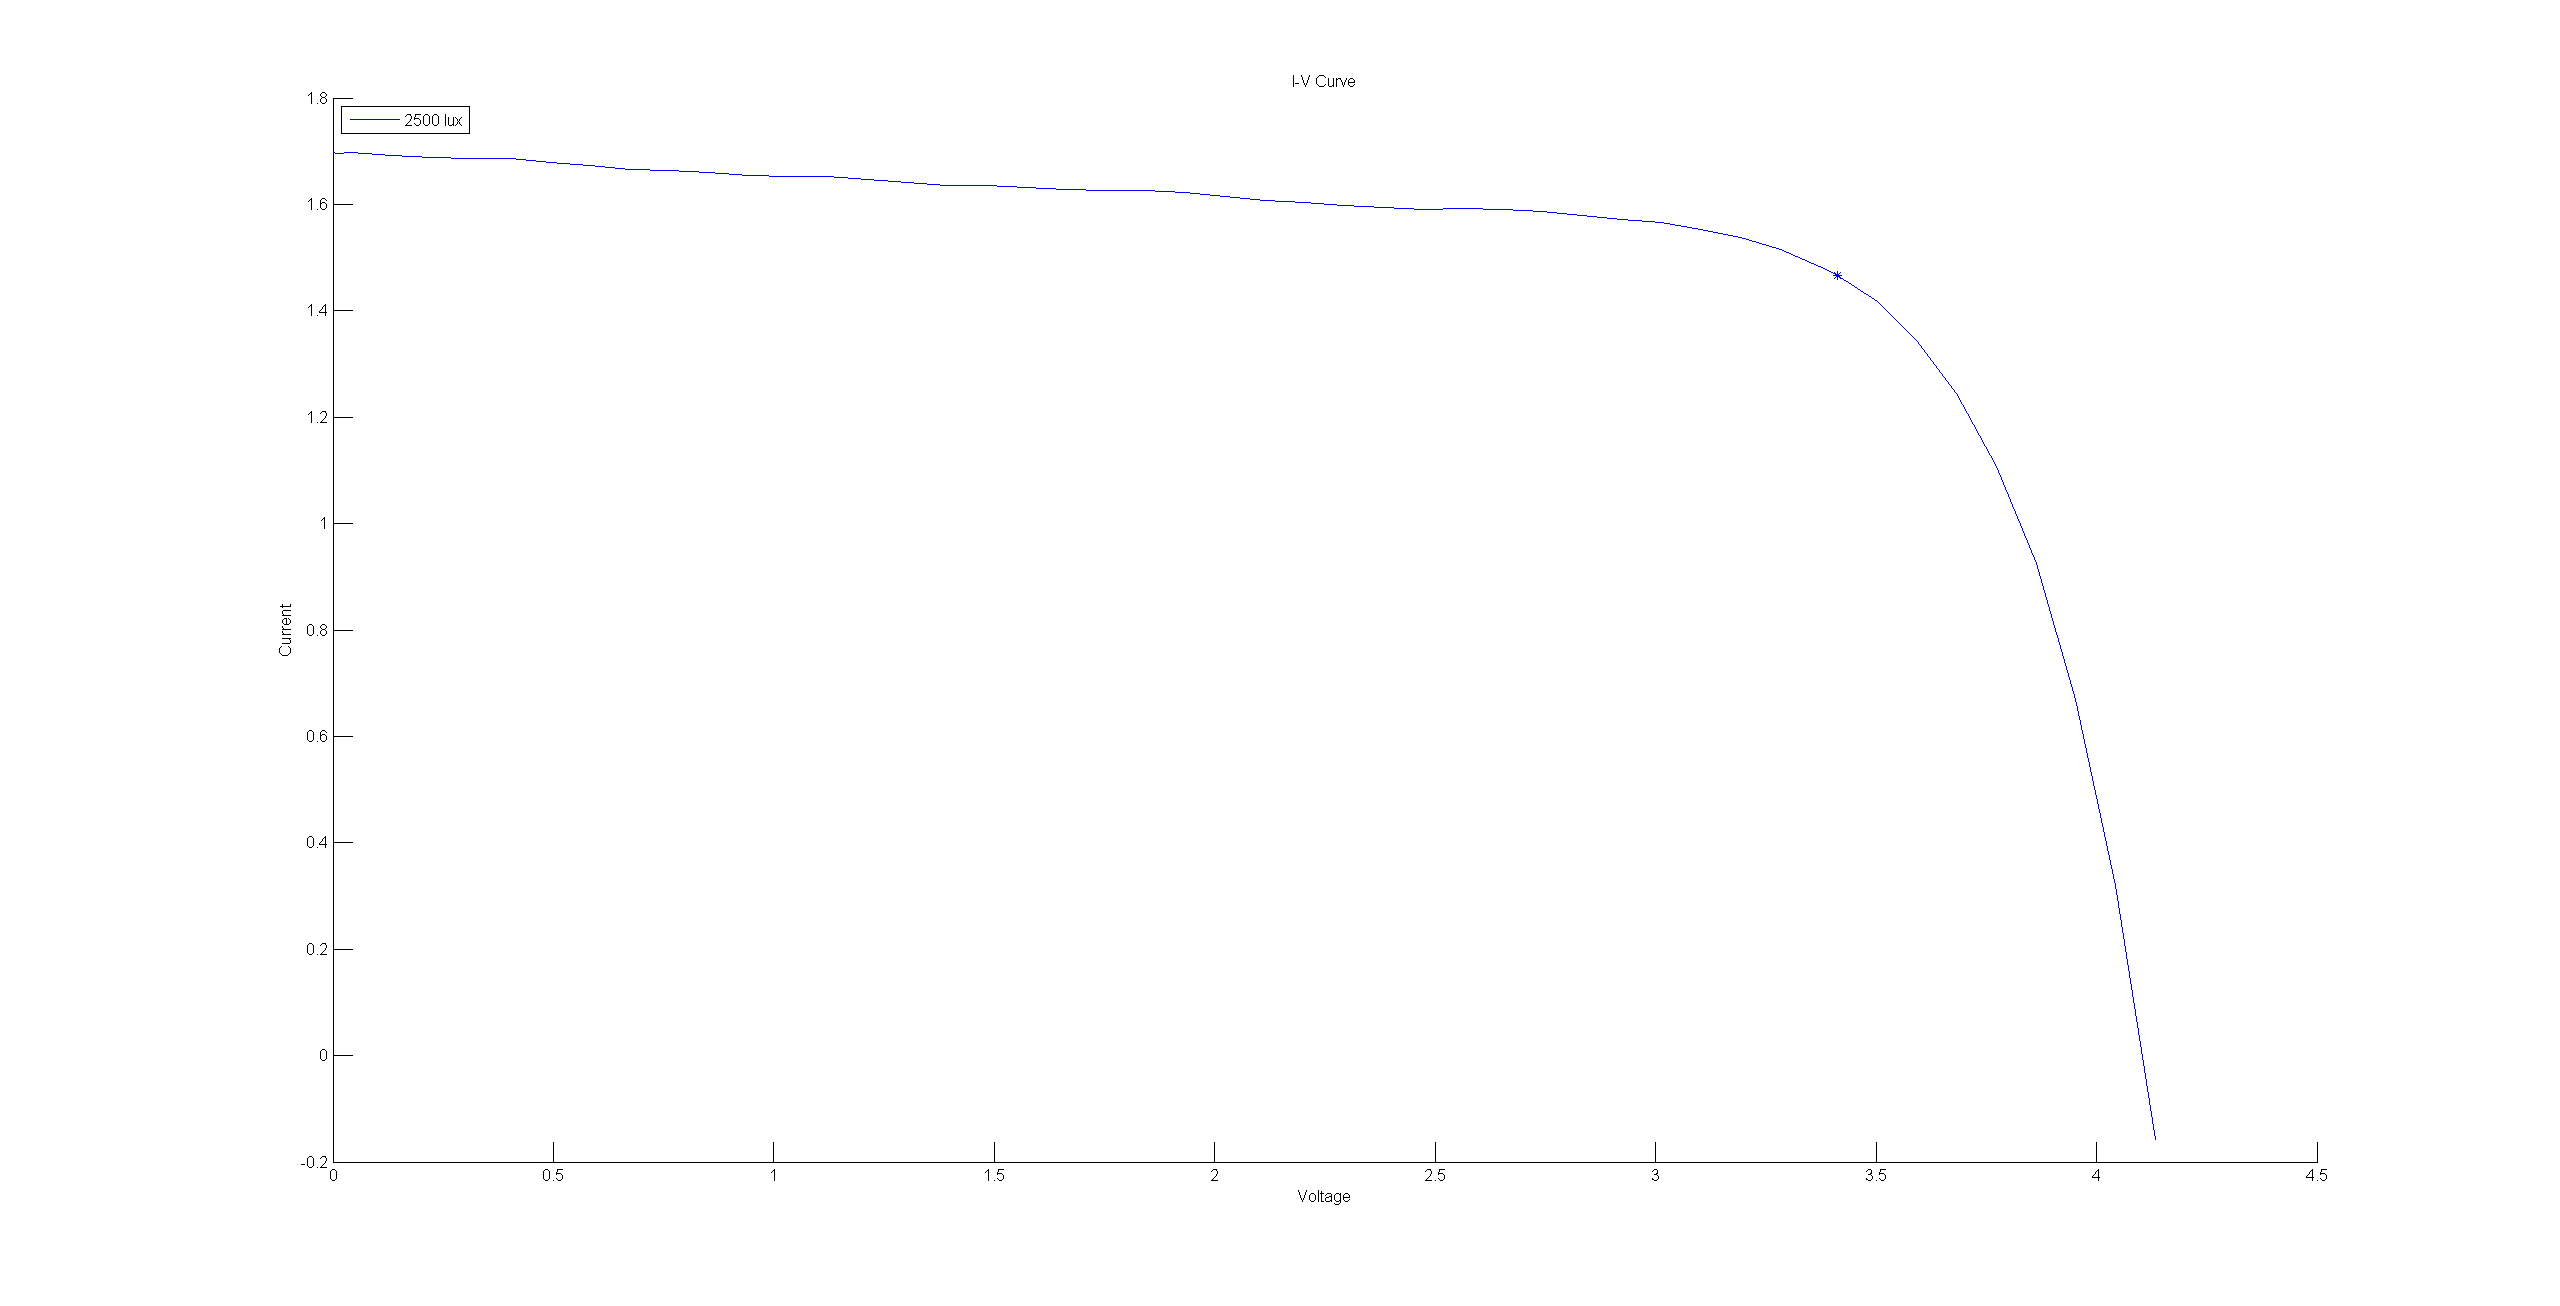
\includegraphics[width=1.1\textwidth]{images/single2500_IV}
		  \caption{I-V curve for the array at steady illumination}
		  \label{fig:2500luxIV}
	  \end{center}
  \end{figure}
  
\begin{figure}[H]
	  \begin{center}
		  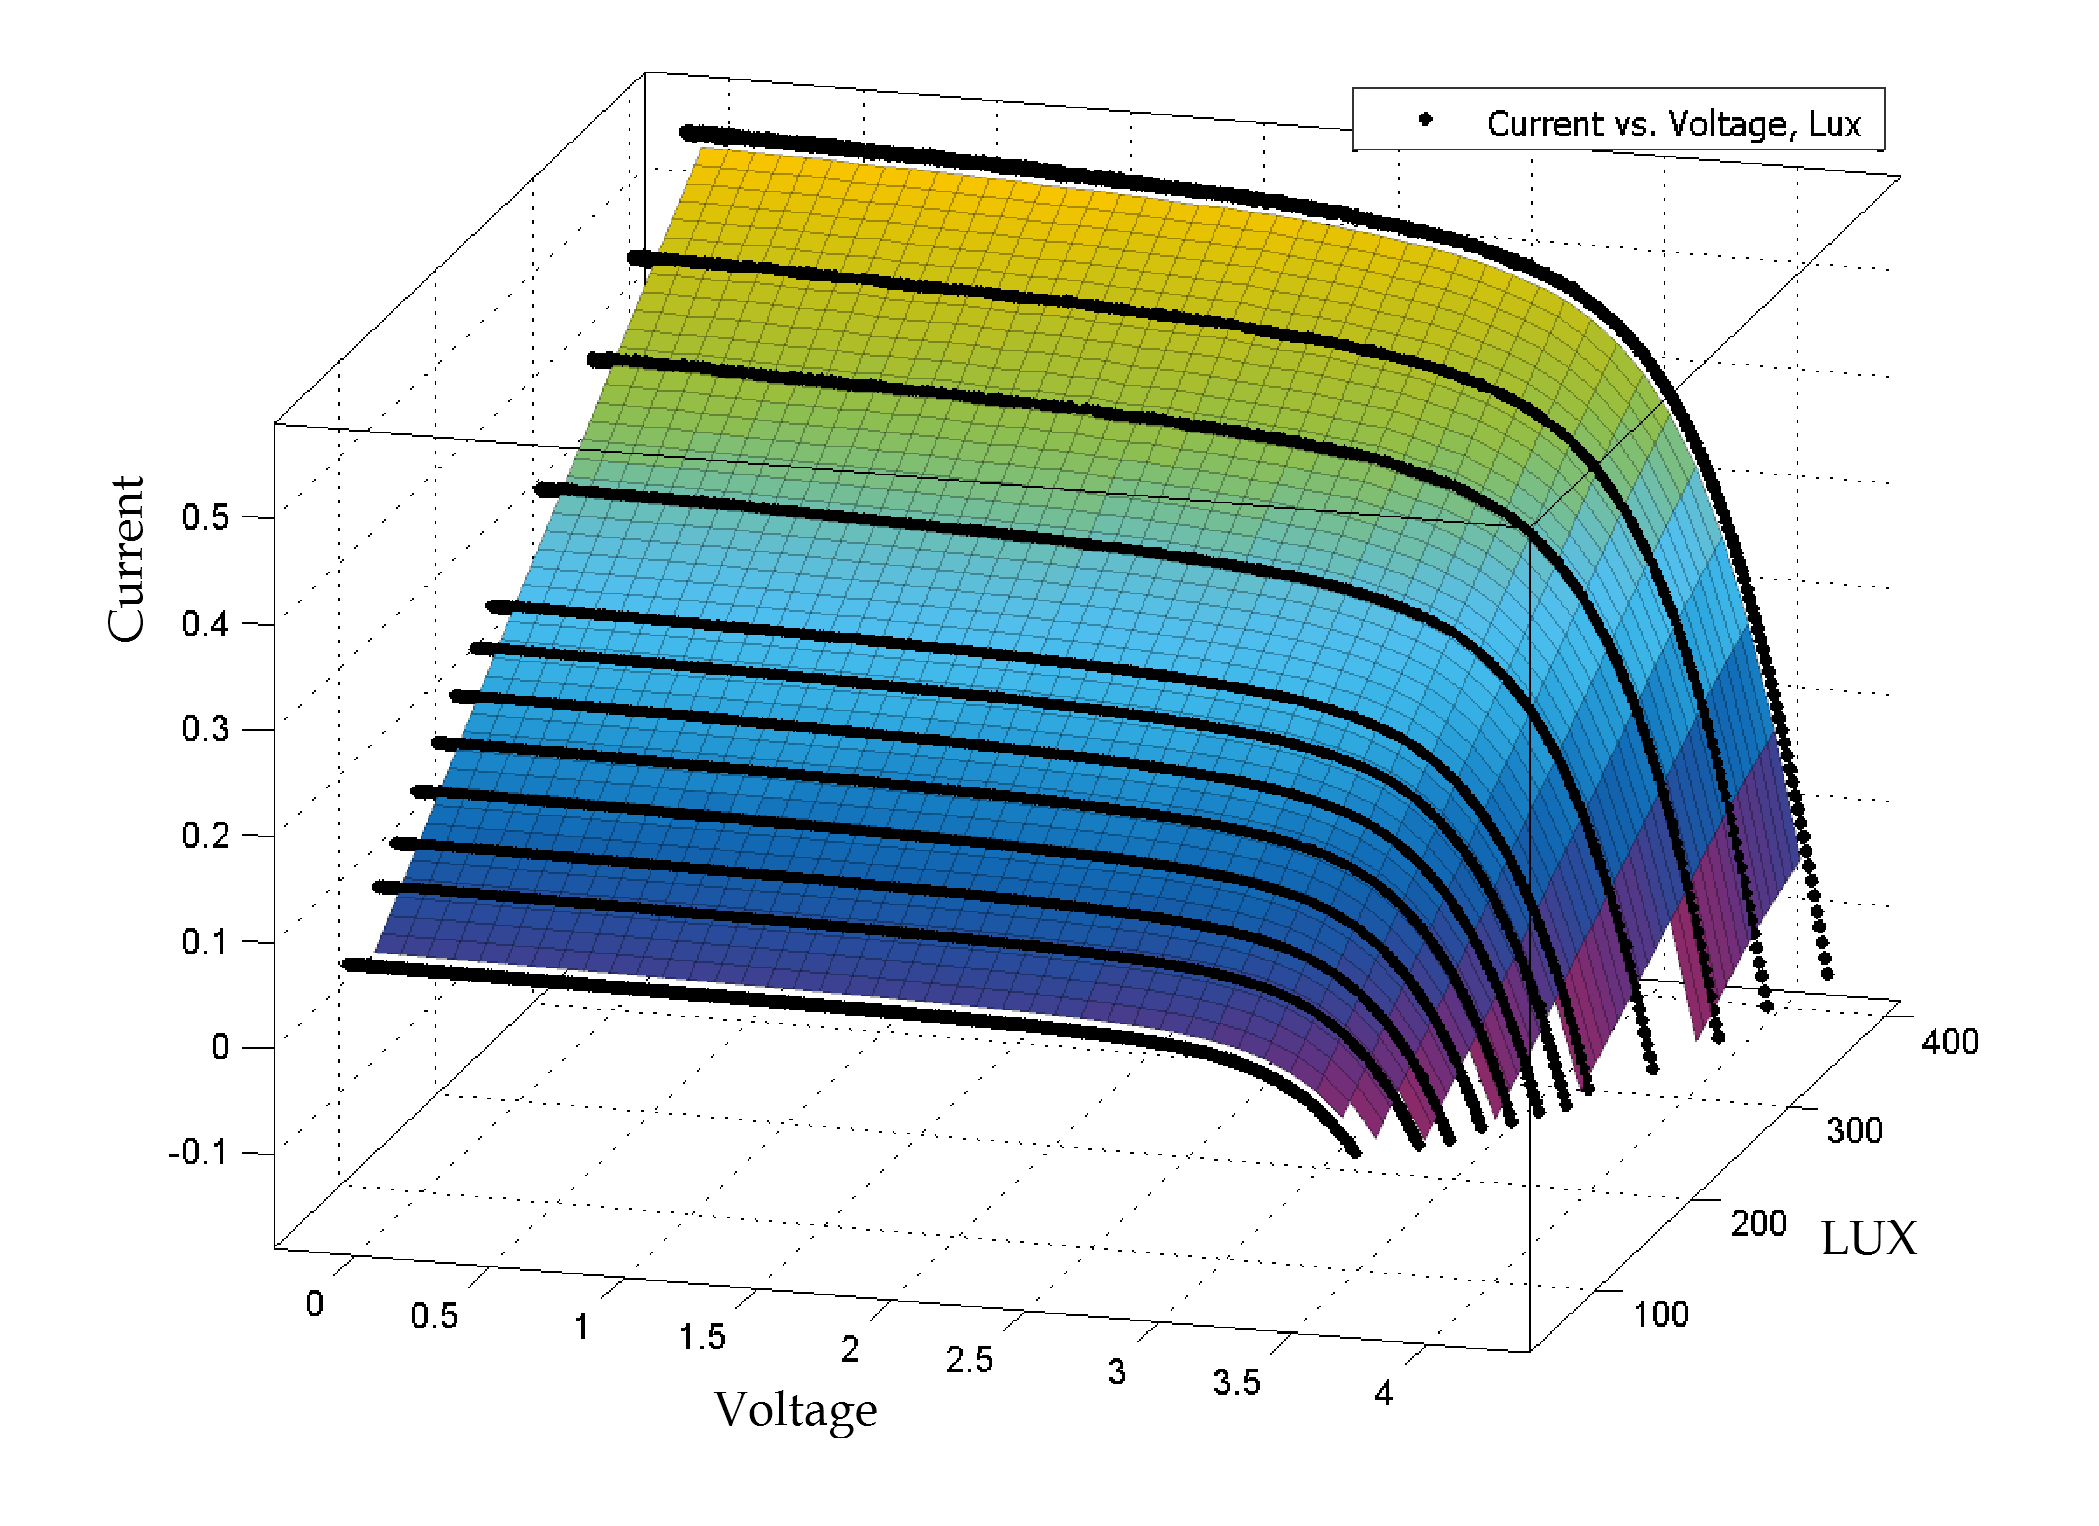
\includegraphics[width=0.8\textwidth]{images/I-V-lux}
		  \caption{I-V curve for the array at varying illumination}
		  \label{fig:luxIV100_2500}
	  \end{center}
  \end{figure}

\section{Modelling and Simulations} 

the three-dimensional surface thus created in the section above acts as a function , a look-up table of sorts. For a given illumination and voltage the function computes a appropriate current value. ** to convert continuous voltage values to discreet values**,a transfer functions are used. Capacitor and diode are added in order to accurately mimic the response of \ac{DSCs} under test as discussed in \ref{sec:SDM} . the \ac{DSCs} subsystem is represented in the figure ~\ref{fig:PV_block_Model} below. This sub-system is placed under a mask in the abstract view shown in figure ~\ref{fig:Model_top} on page ~\pageref{fig:Model_top} in order to simplify operation and for ** ascetic ** reasons. The validation of the said model is discussed in section \ref{sec:Validation}.\\

The \textit{Scopes and Outputs} subsection is used to plot data on to graphs and to push data onto Matlab for further analysis.\\

\textit{\ac{MPPT} Controller Block}

\begin{figure}[H]
	  \begin{center}
		  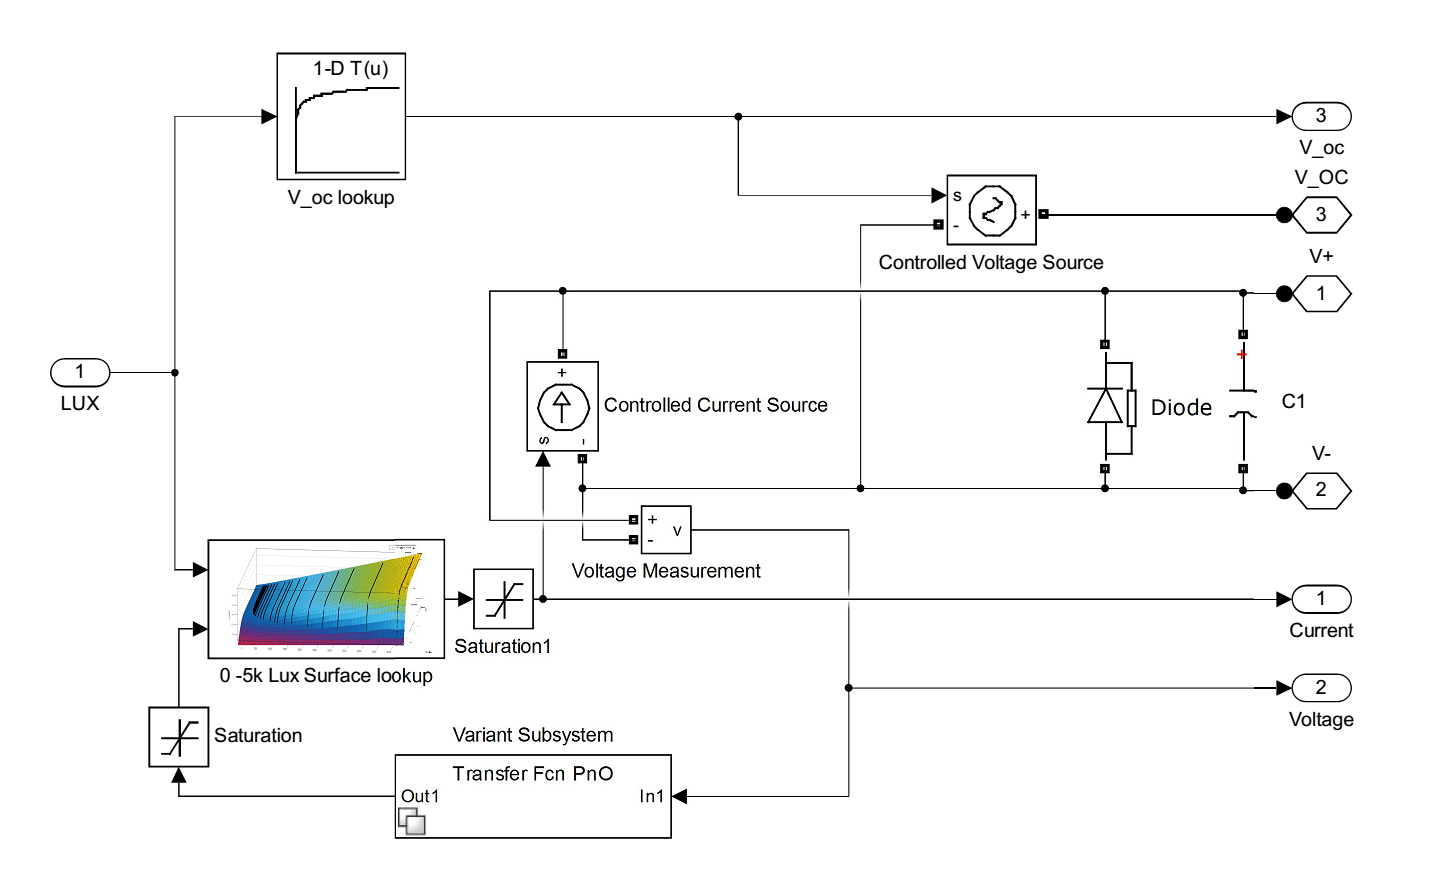
\includegraphics[width=\textwidth]{images/PV_block_Model}
		  \caption{Modelling of the DSC Subsystem }
		  \label{fig:PV_block_Model}
	  \end{center}
  \end{figure}

\begin{figure}[H]
  \begin{center}
	  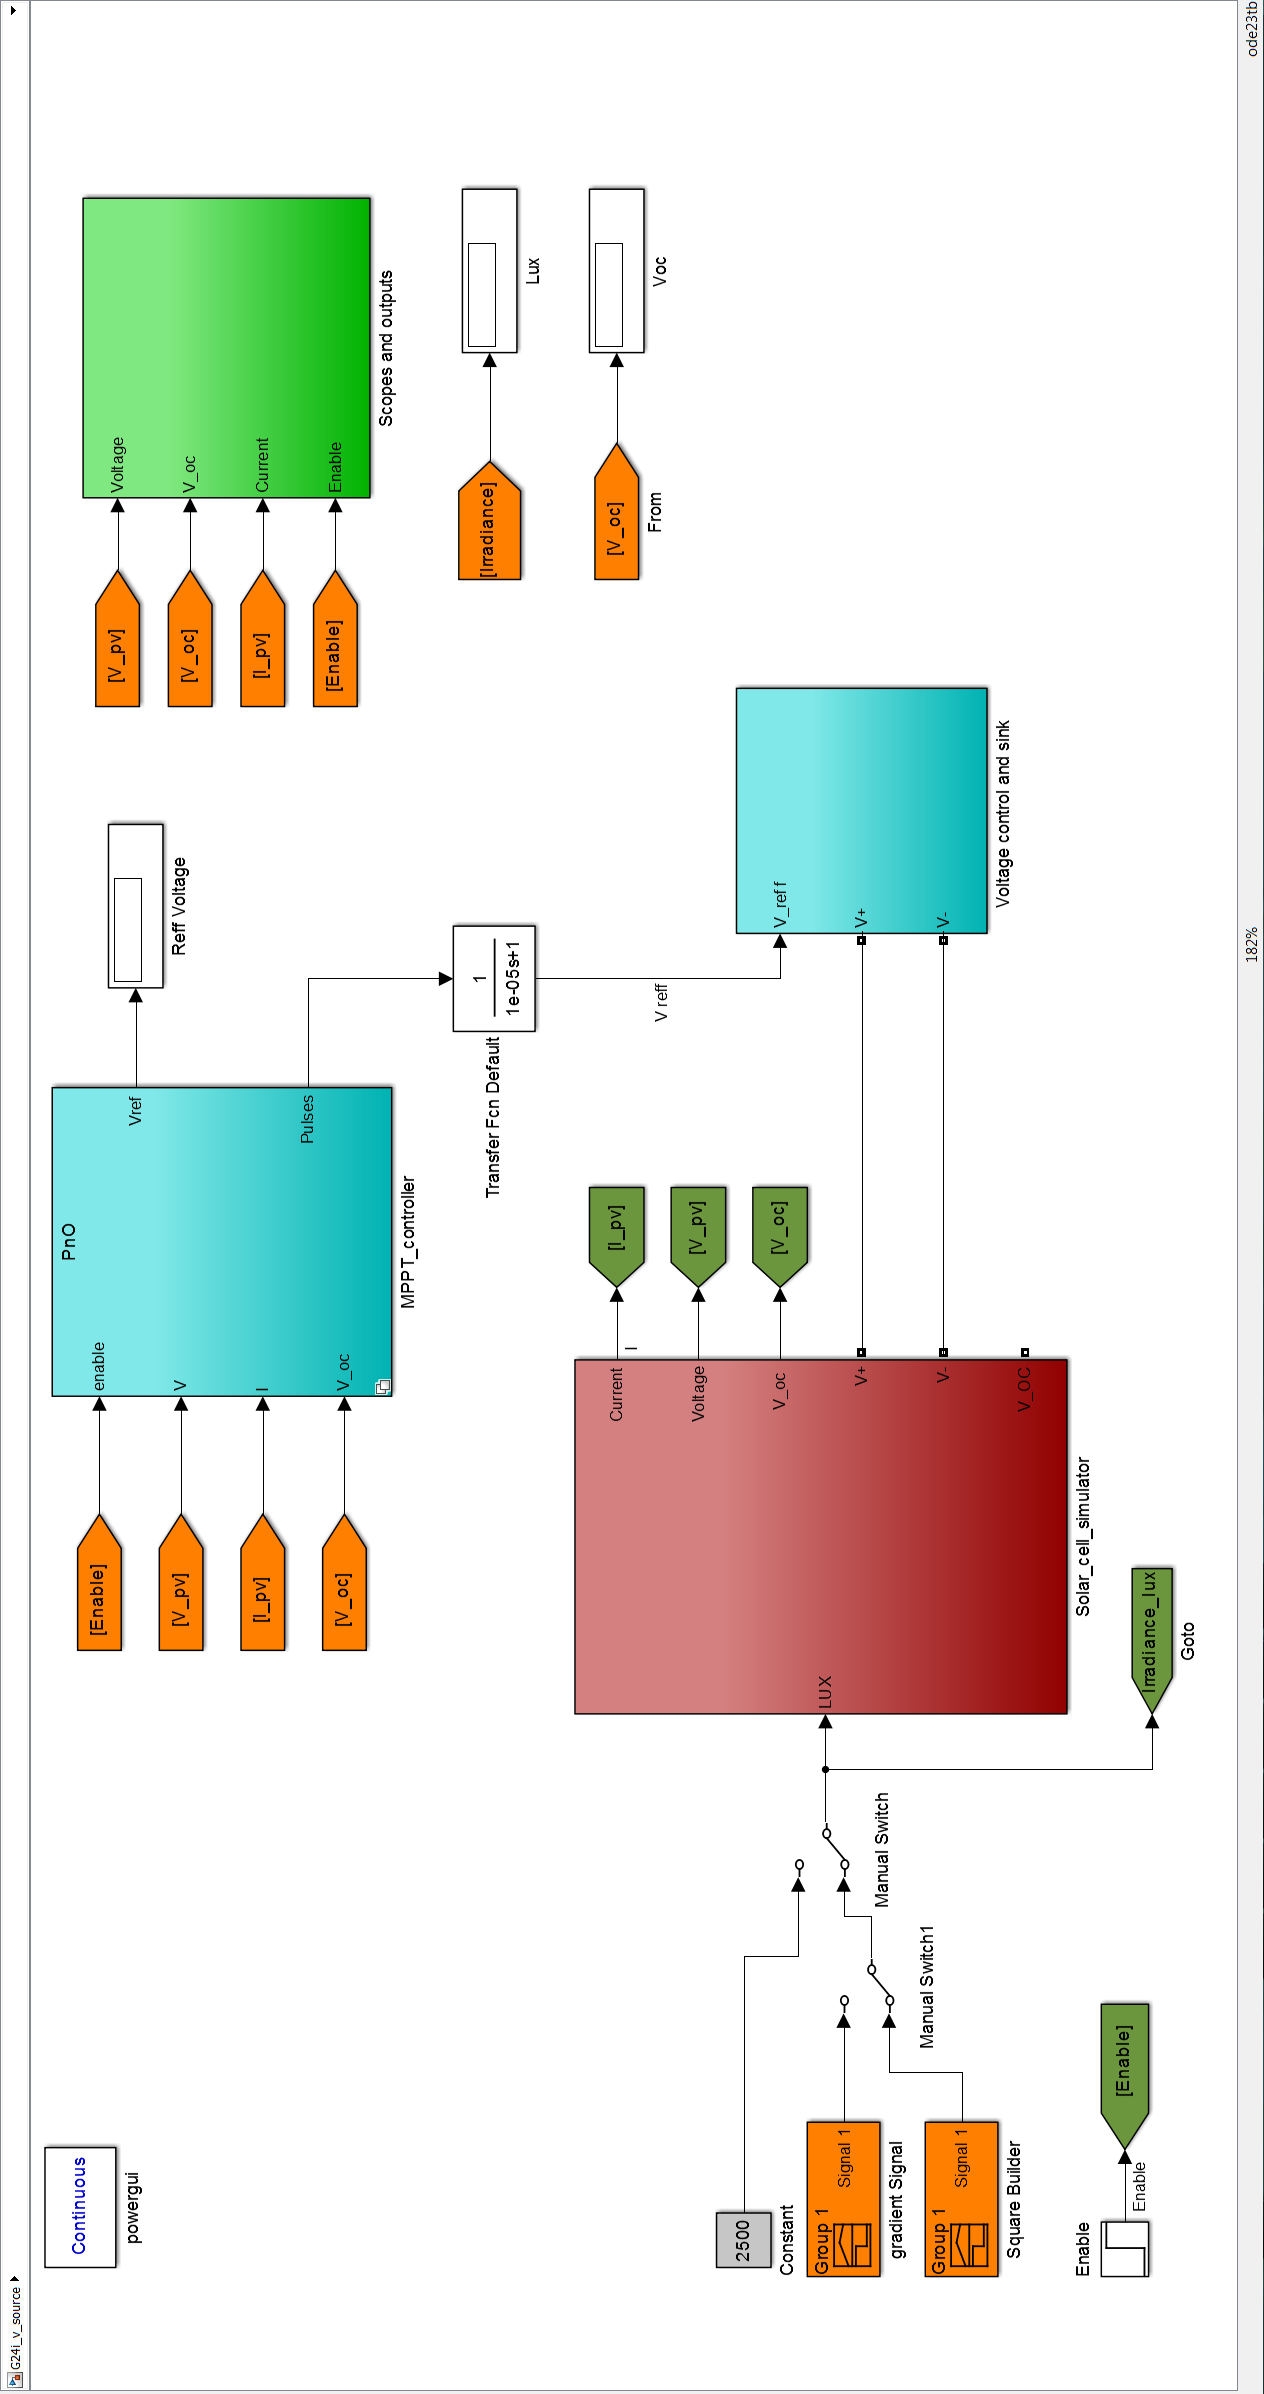
\includegraphics[width=0.8\textwidth]{images/Top_level_mod}
	  \caption{Top Model }
	  \label{fig:Model_top}
  \end{center}
\end{figure}

\begin{figure}[H]
  \begin{center}
	  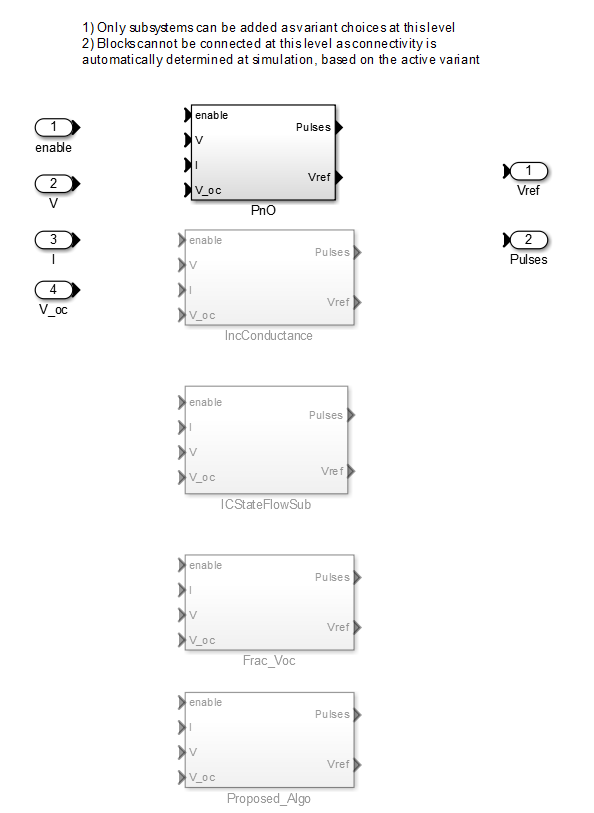
\includegraphics[width=\textwidth]{images/controller_mod}
	  \caption{MPPT controller }
	  \label{fig:Controller_mod}
  \end{center}
\end{figure}
 



\section {Validation of the model in Matlab{\textregistered}}\label{sec:Validation} 

\begin{figure}[H]
	  \begin{center}
		  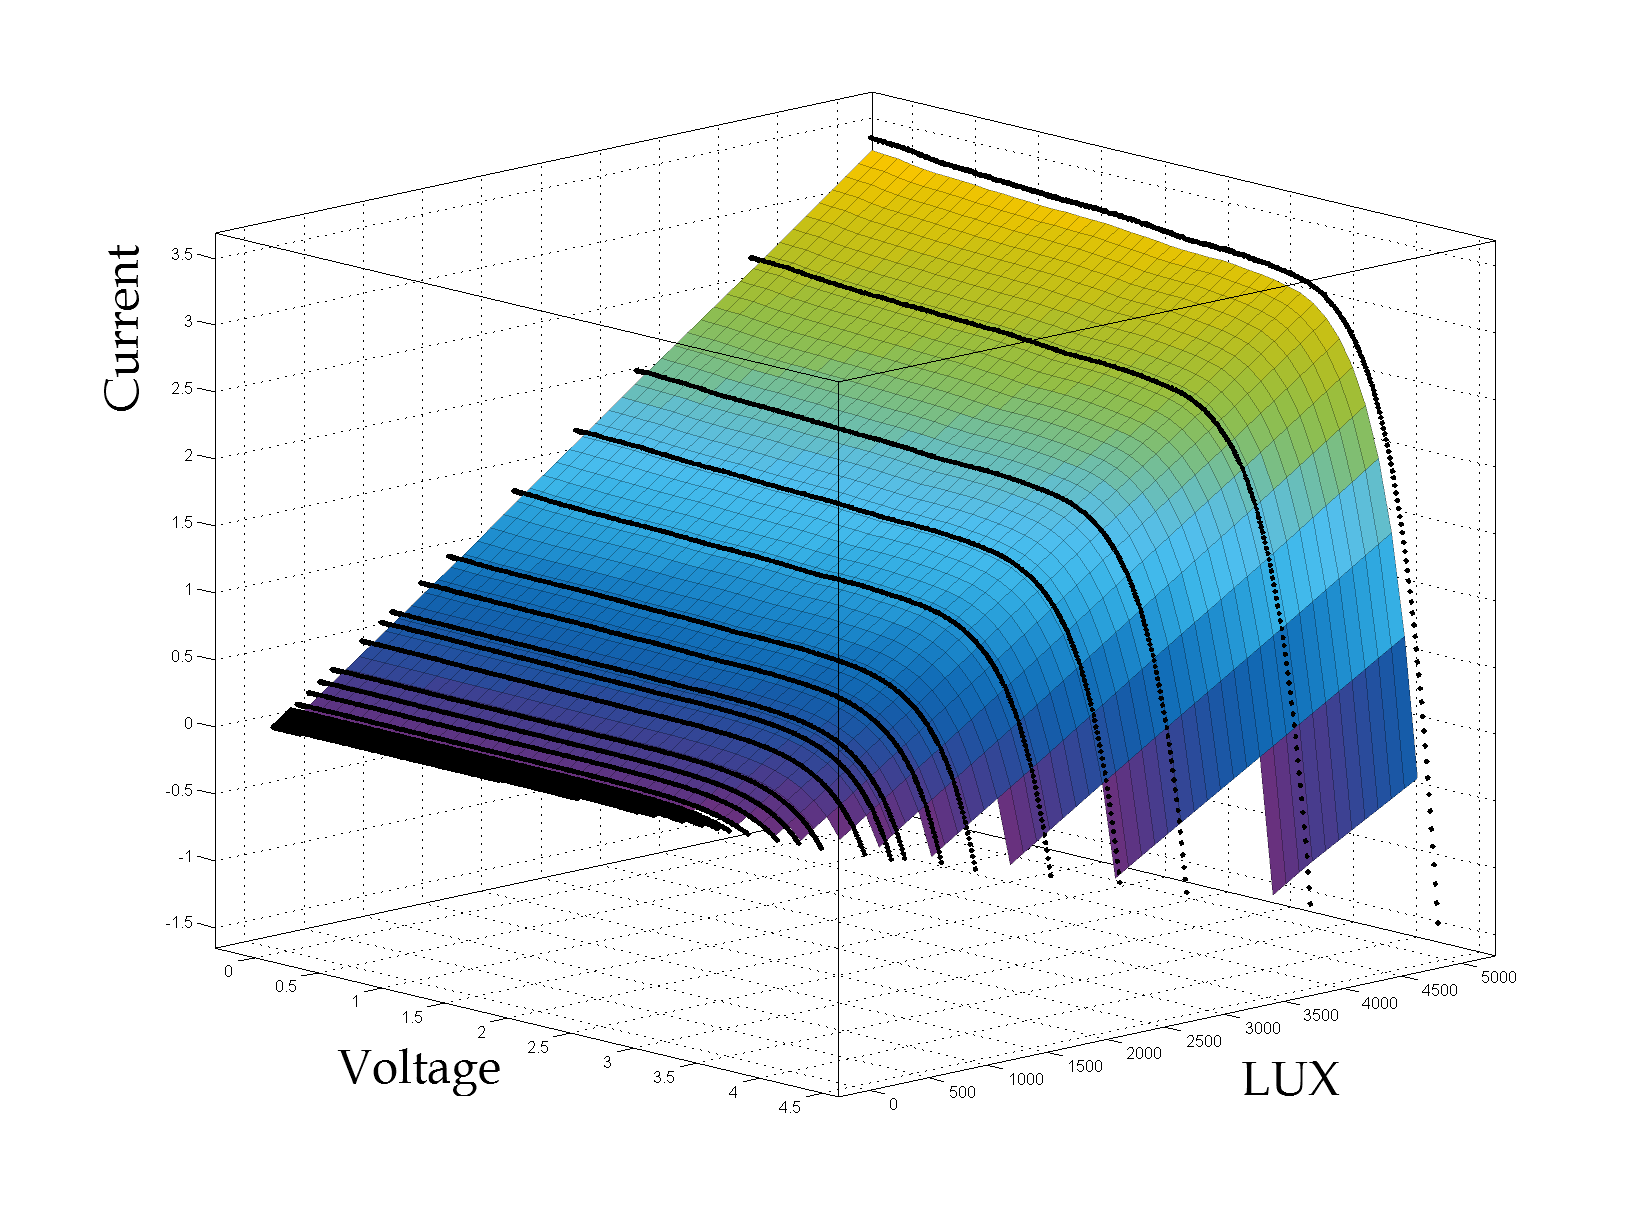
\includegraphics[width=0.8\textwidth]{images/IVLUX_LAB_measured}
		  \caption{Modelling of the DSC Subsystem }
		  \label{fig:IVLUX_LAB_measured}
	  \end{center}
  \end{figure}

\begin{figure}[H]
  \begin{center}
	  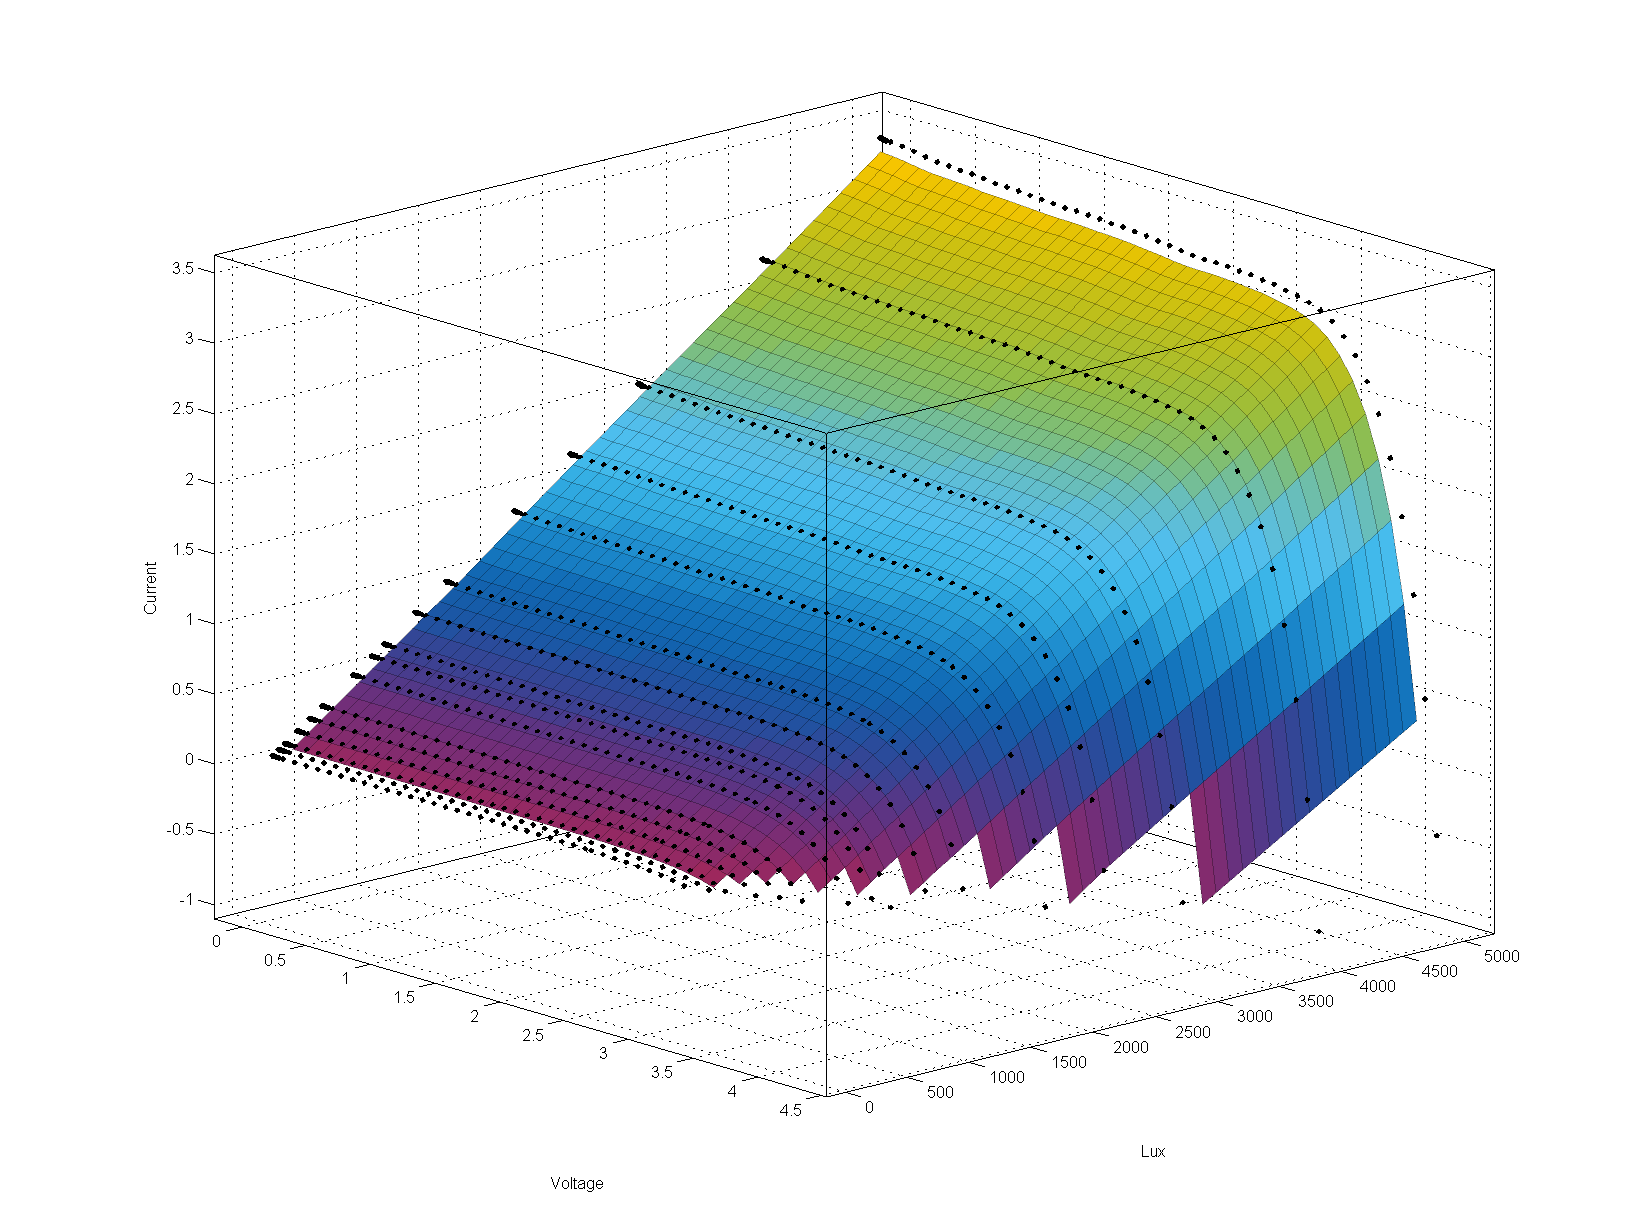
\includegraphics[width=0.8\textwidth]{images/IVLUX_MOD_gen}
	  \caption{Top Model }
	  \label{fig:IVLUX_MOD_gen}
  \end{center}
\end{figure}

\begin{figure}[H]
  \begin{center}
	  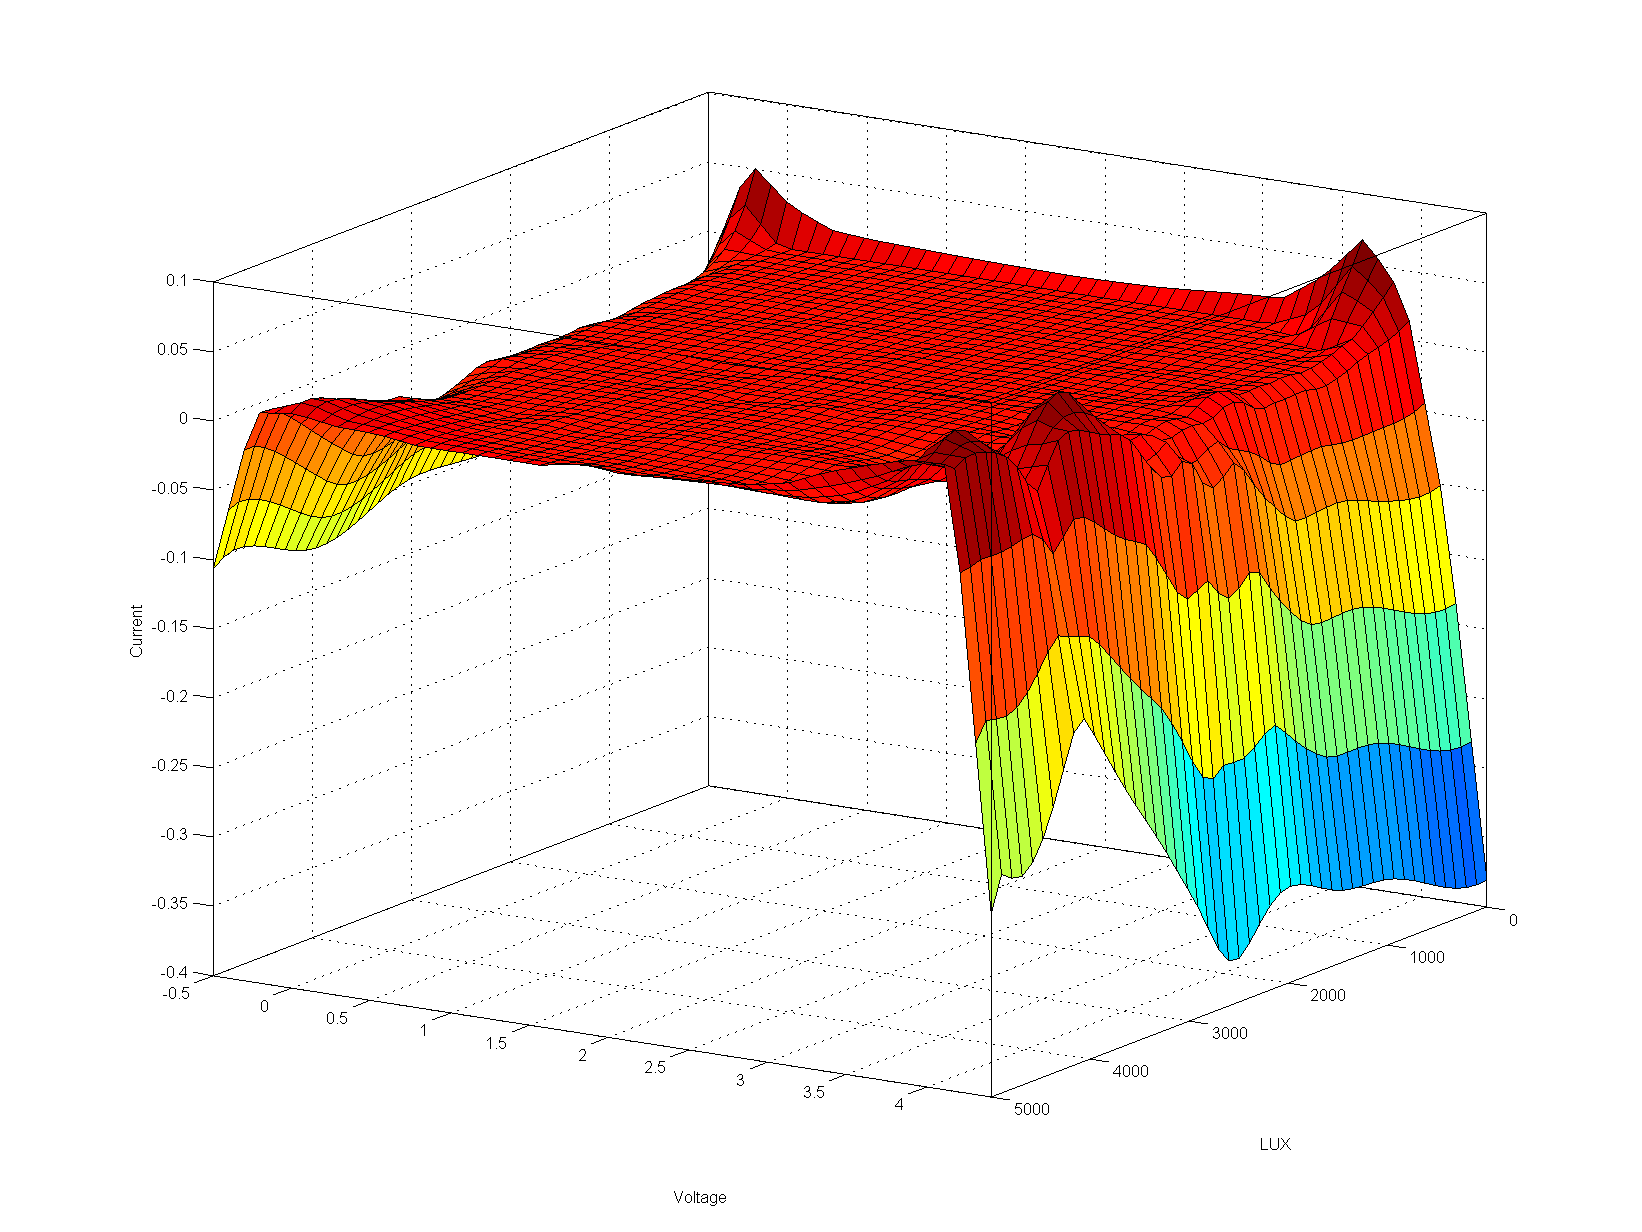
\includegraphics[width=\textwidth]{images/Diff_Contour}
	  \caption{Top Model }
	  \label{fig:Diff_Contour}
  \end{center}
\end{figure}

\begin{figure}[H]
  \begin{center}
	  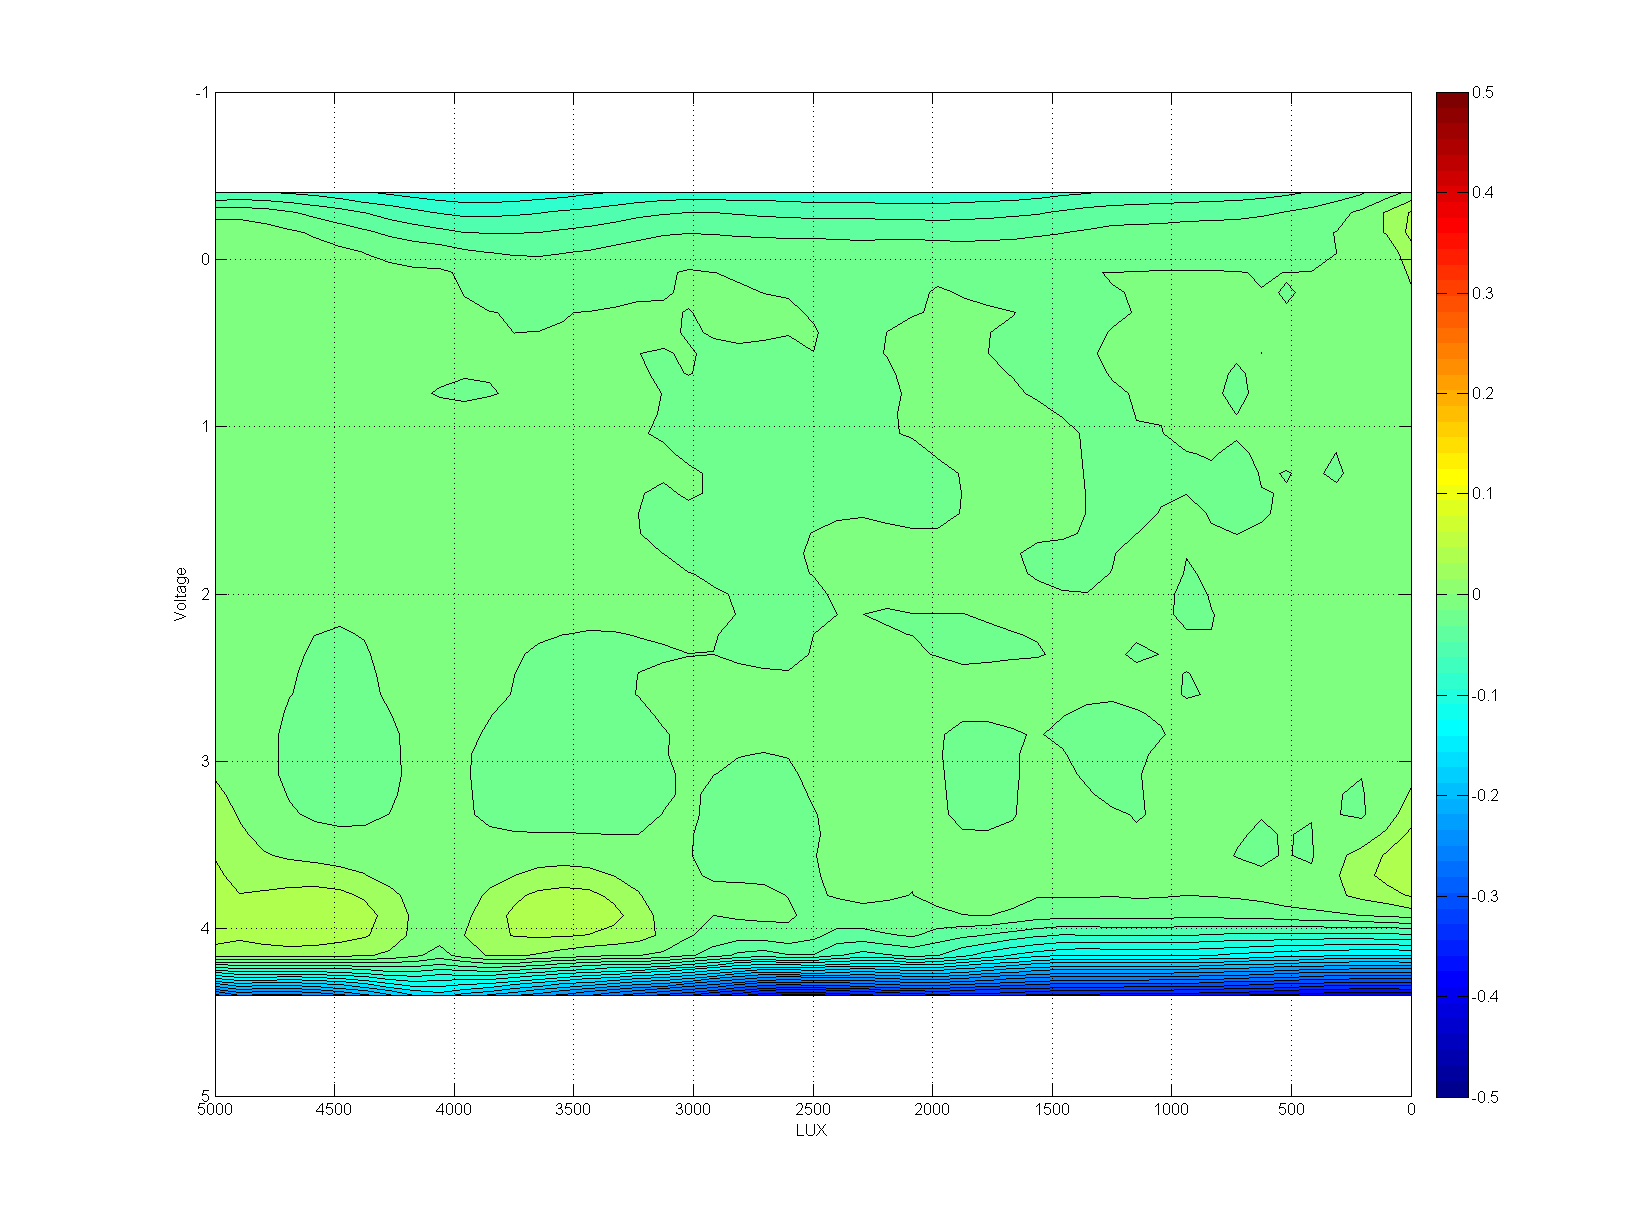
\includegraphics[width=\textwidth]{images/Contour_map}
	  \caption{Top Model }
	  \label{fig:Contour_map}
  \end{center}
\end{figure}

\section{Proposed Method }

\cite{houssamo2013experimental}

This work presents an experimental comparison; Using four identical PV, under strictly the same set of technical and meteorological conditions, an experimental comparison  of four most used MPPT methods for PV power systems is done.This comparison shows the advantage of use of a MPPT with a variable tracking step.\\  

\cite{jain2004new}
This paper presents a new algorithm for tracking maximum power point in photovoltaic systems. This is a fast tracking algorithm, where an initial approximation of \ac{MPP} quickly achieved using a variable step-size. Subsequently, the exact\ac{MPP} can be targeted using any conventional method like the hill-climbing or incremental conductance method. Thus, the drawback of a fixed small step-size over the entire tracking range is removed, resulting in reduced number of iterations and much faster tracking compared to conventional methods. \\
 My implementation draws inspiration for the above article for its  two-stage algorithm to reduce the number of iterations but deviates significantly in the implementation and algorithms used to identify the \ac{MPP} 
 
\cite{liu2011fast}

\begin{figure}[H]
  \begin{center}
	  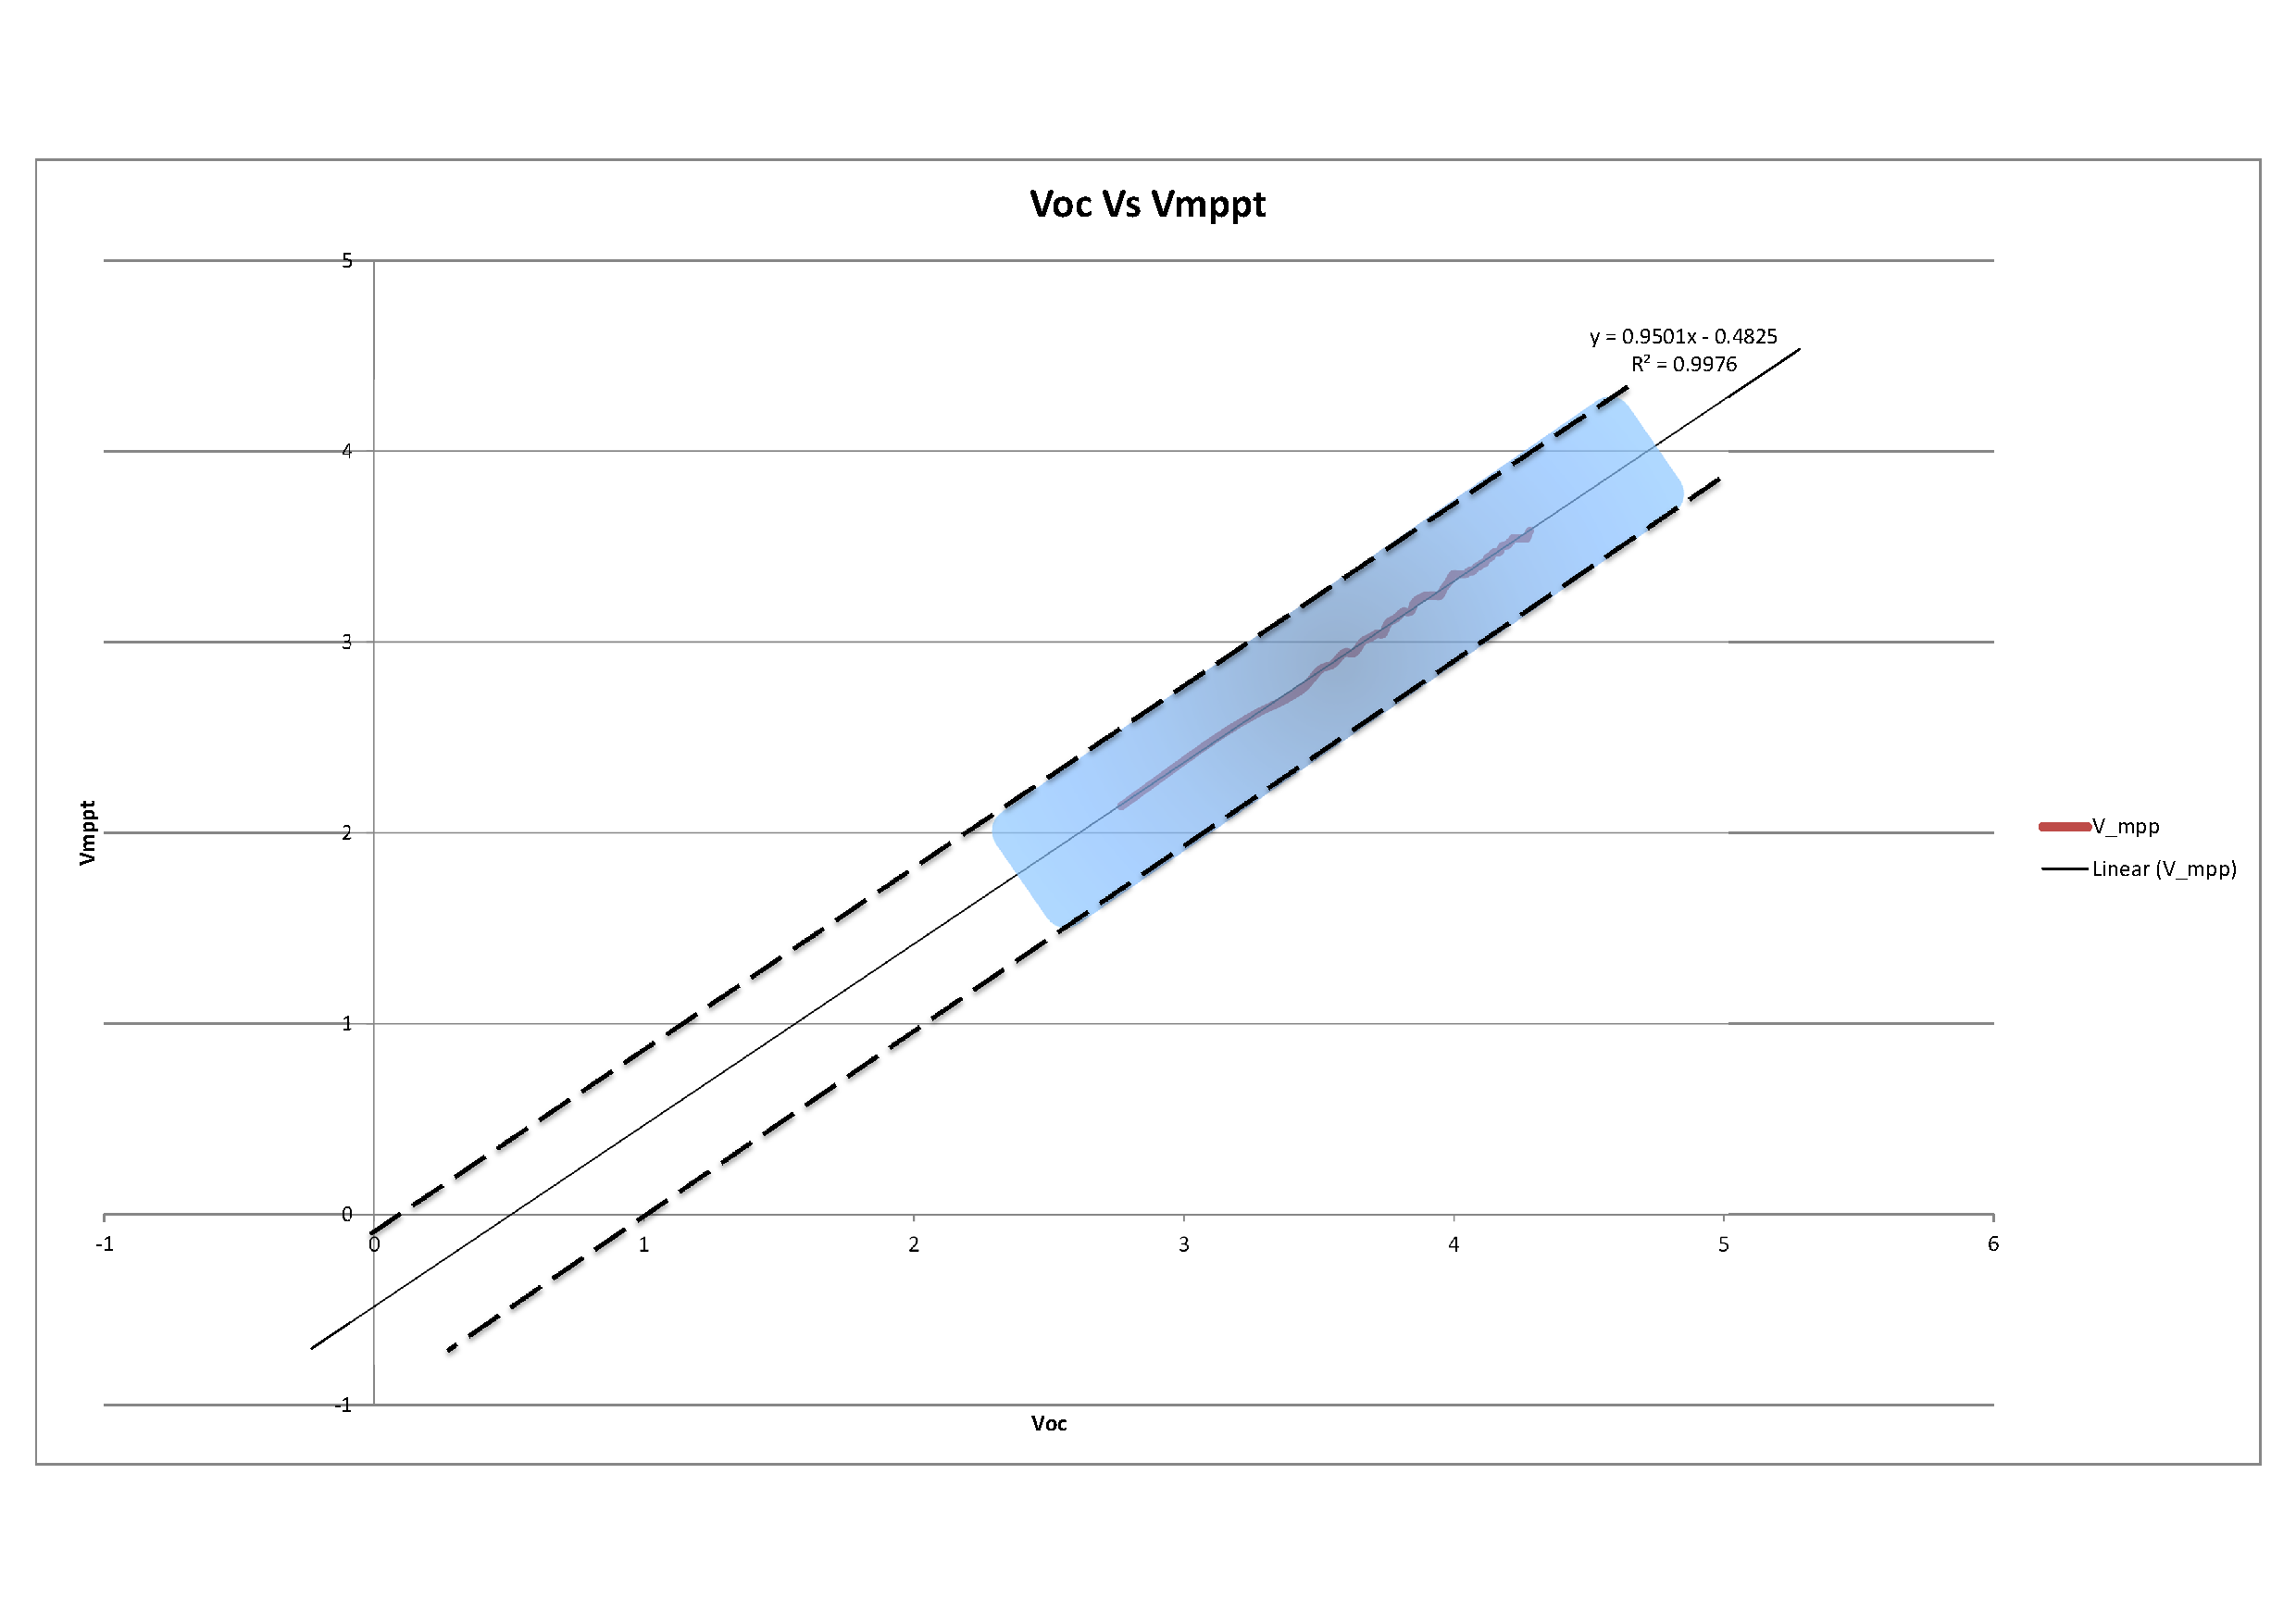
\includegraphics[width=1.1\textwidth]{images/Probability_field}
	  \caption{Probability field }
	  \label{fig:Probability_field}
  \end{center}
\end{figure}

  \begin{figure}[H]
    \begin{center}
	   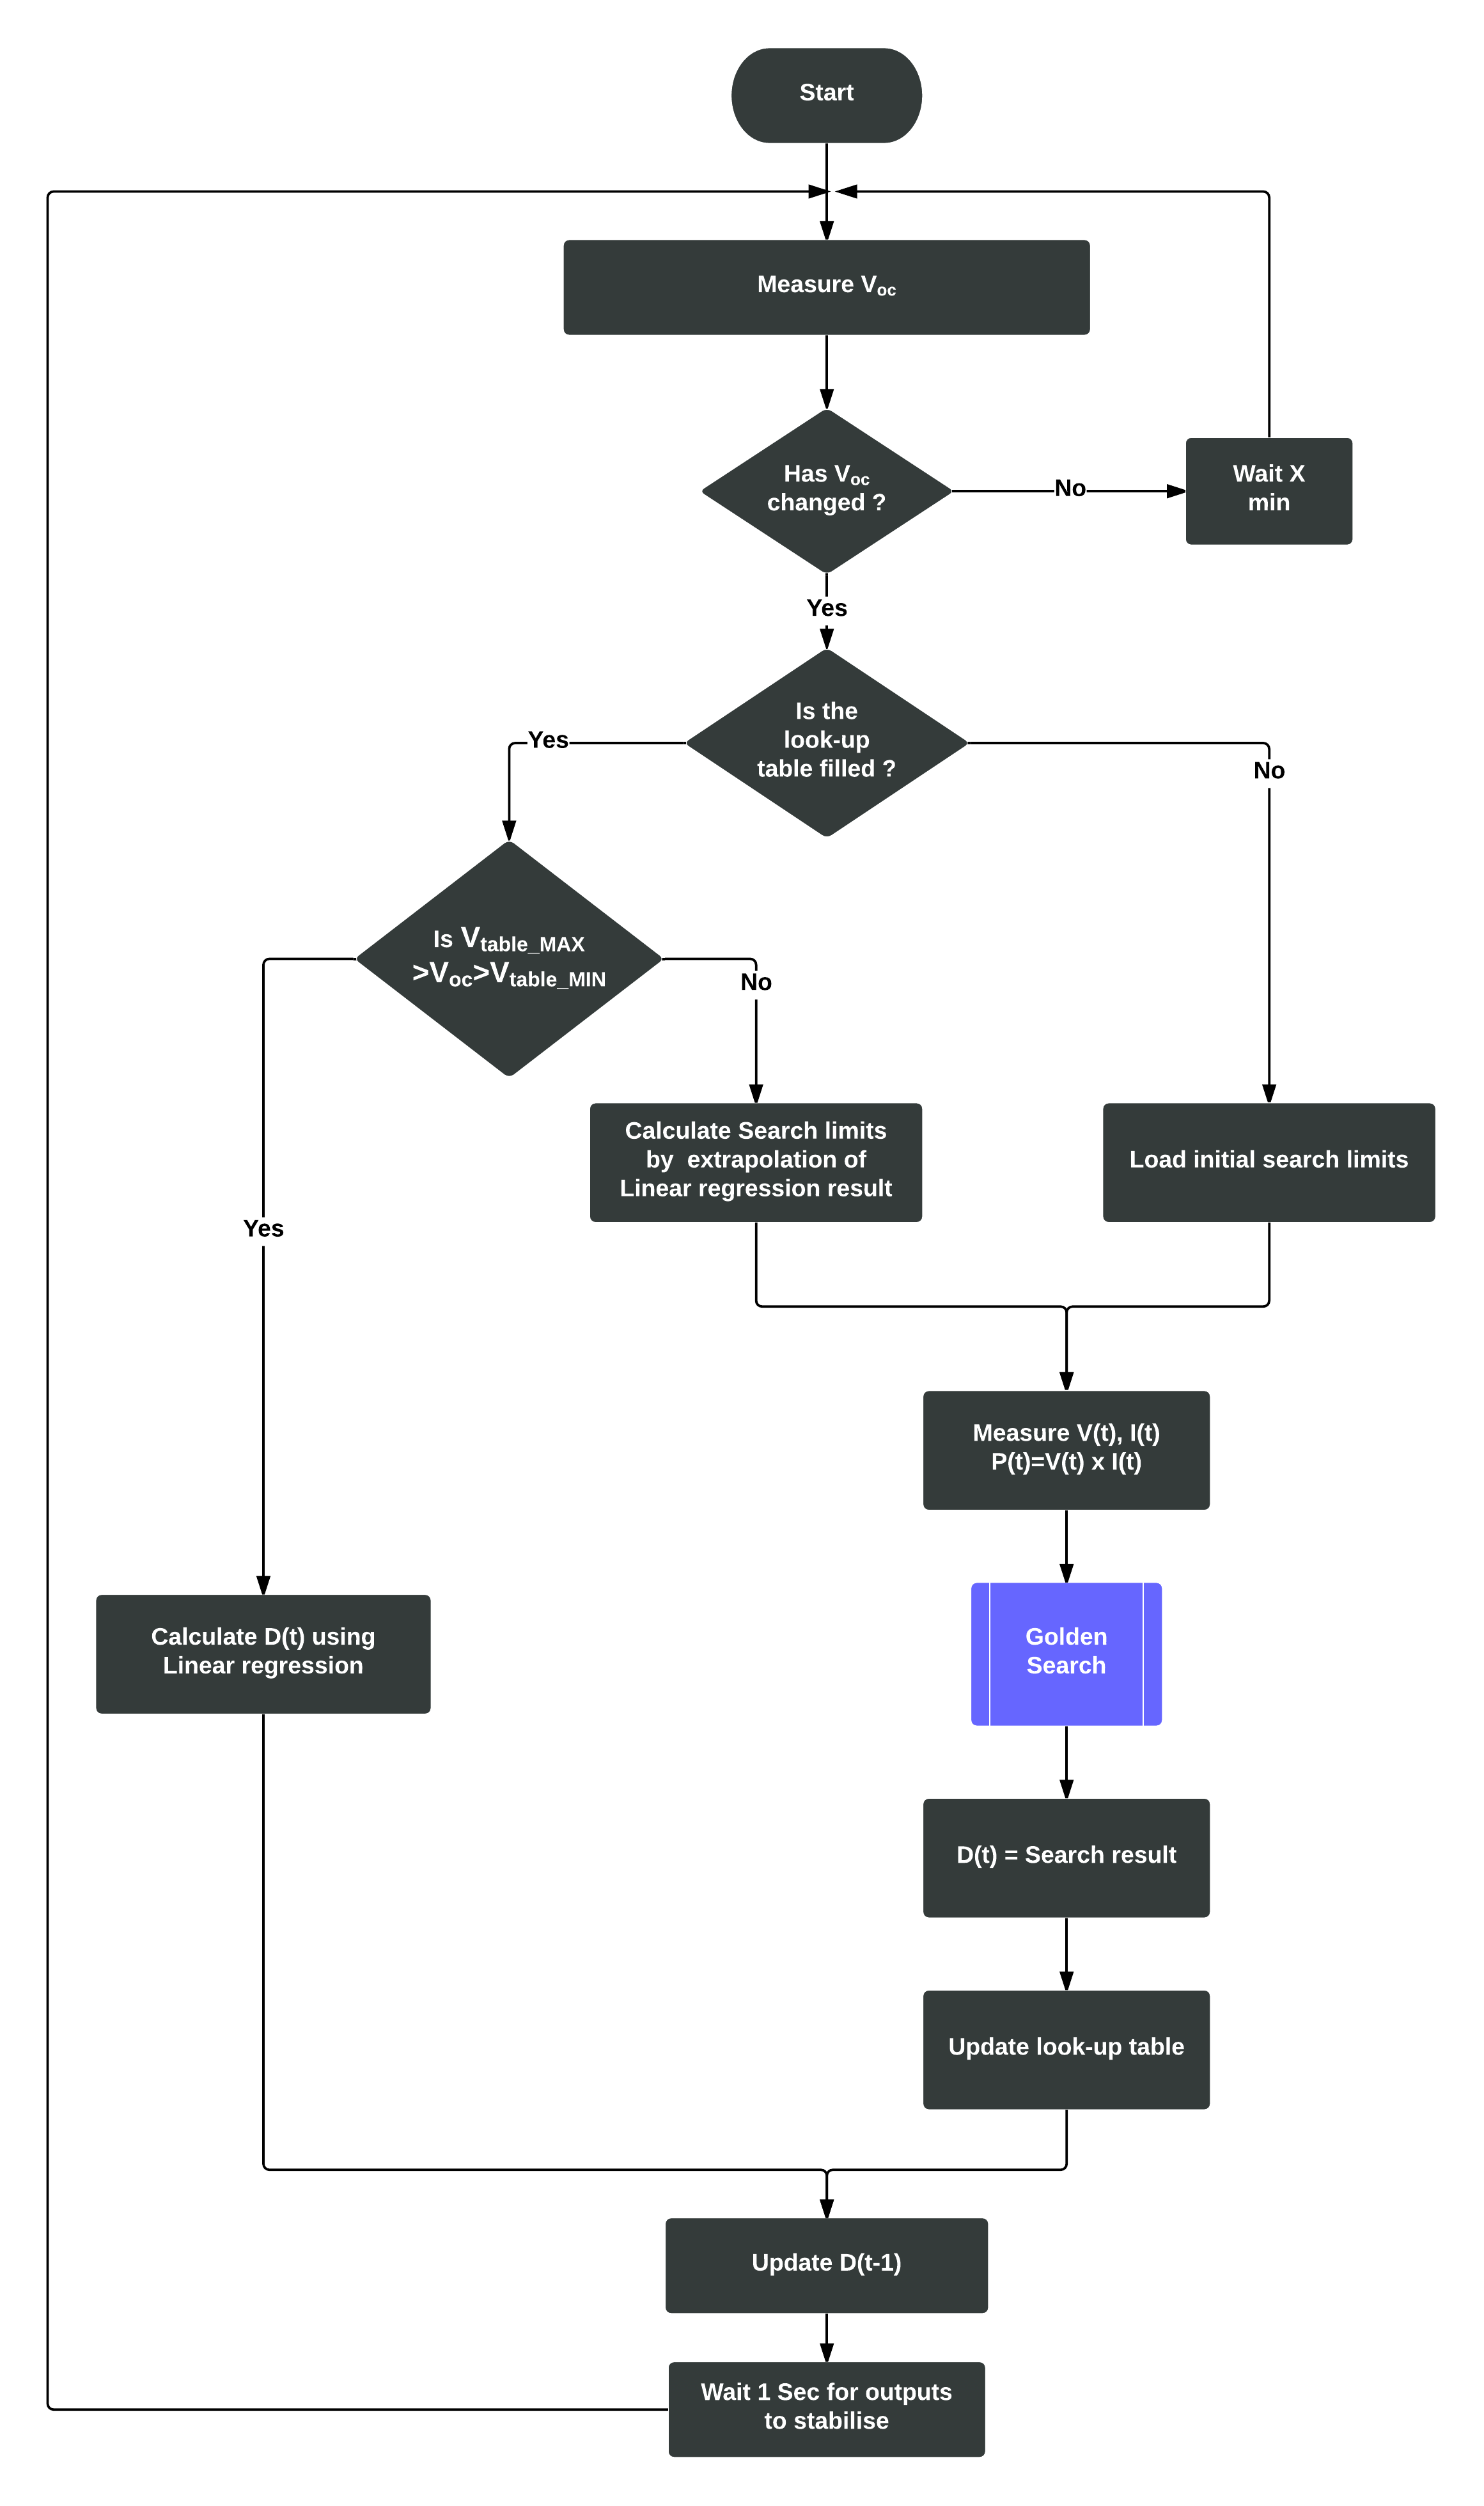
\includegraphics[width=0.9\textwidth]{images/Proposed_Flow}
	   \caption{ Flow chart for Proposed MPPT Algorithm }
	   \label{fig:cyflow}
    \end{center}
  \end{figure}






    \chapter{Result Discussion}
 
 \section{Perturb and Observe Method }
 
 The \ac{PnO} algorithm works by periodicity perturbing the cell and observing the direction of the change in power and consequently moving the $V\textsubscript{ref}$ in the same direction. The $V\textsubscript{ref}$ is moved in small increments or decrements depending on power change.
 However we soon come to realise that true \ac{MPP} is never reached and multiple iterations are required to even reach close. Due to the capacitive effect seen in \ac{DSCs}, the cells are very slow to respond to any change in operating voltage necessitating a rest period for the cells to stabilise which could vary from 500 ms to a few seconds between each step. Under such conditions the numerous iterations mandated by the \ac{PnO} method could potentially mean its several minuets before the operating point is anywhere close to the \ac{MPP}, assuming of course that the solar irradiation remains constant during this search. 
 
 The Lower graph in figure~\ref{fig:PnO_result} on page~\pageref{fig:PnO_result} is the input to the model, simulating the change in incident irradiation and the top graph in blue represents input power of the solar cell. It is interesting to observe that this implementation of \ac{PnO} had trouble locking on to the \ac{MPP} during gradually incrementing light conditions.                       
  \begin{figure}[H]
	   \begin{center}
		   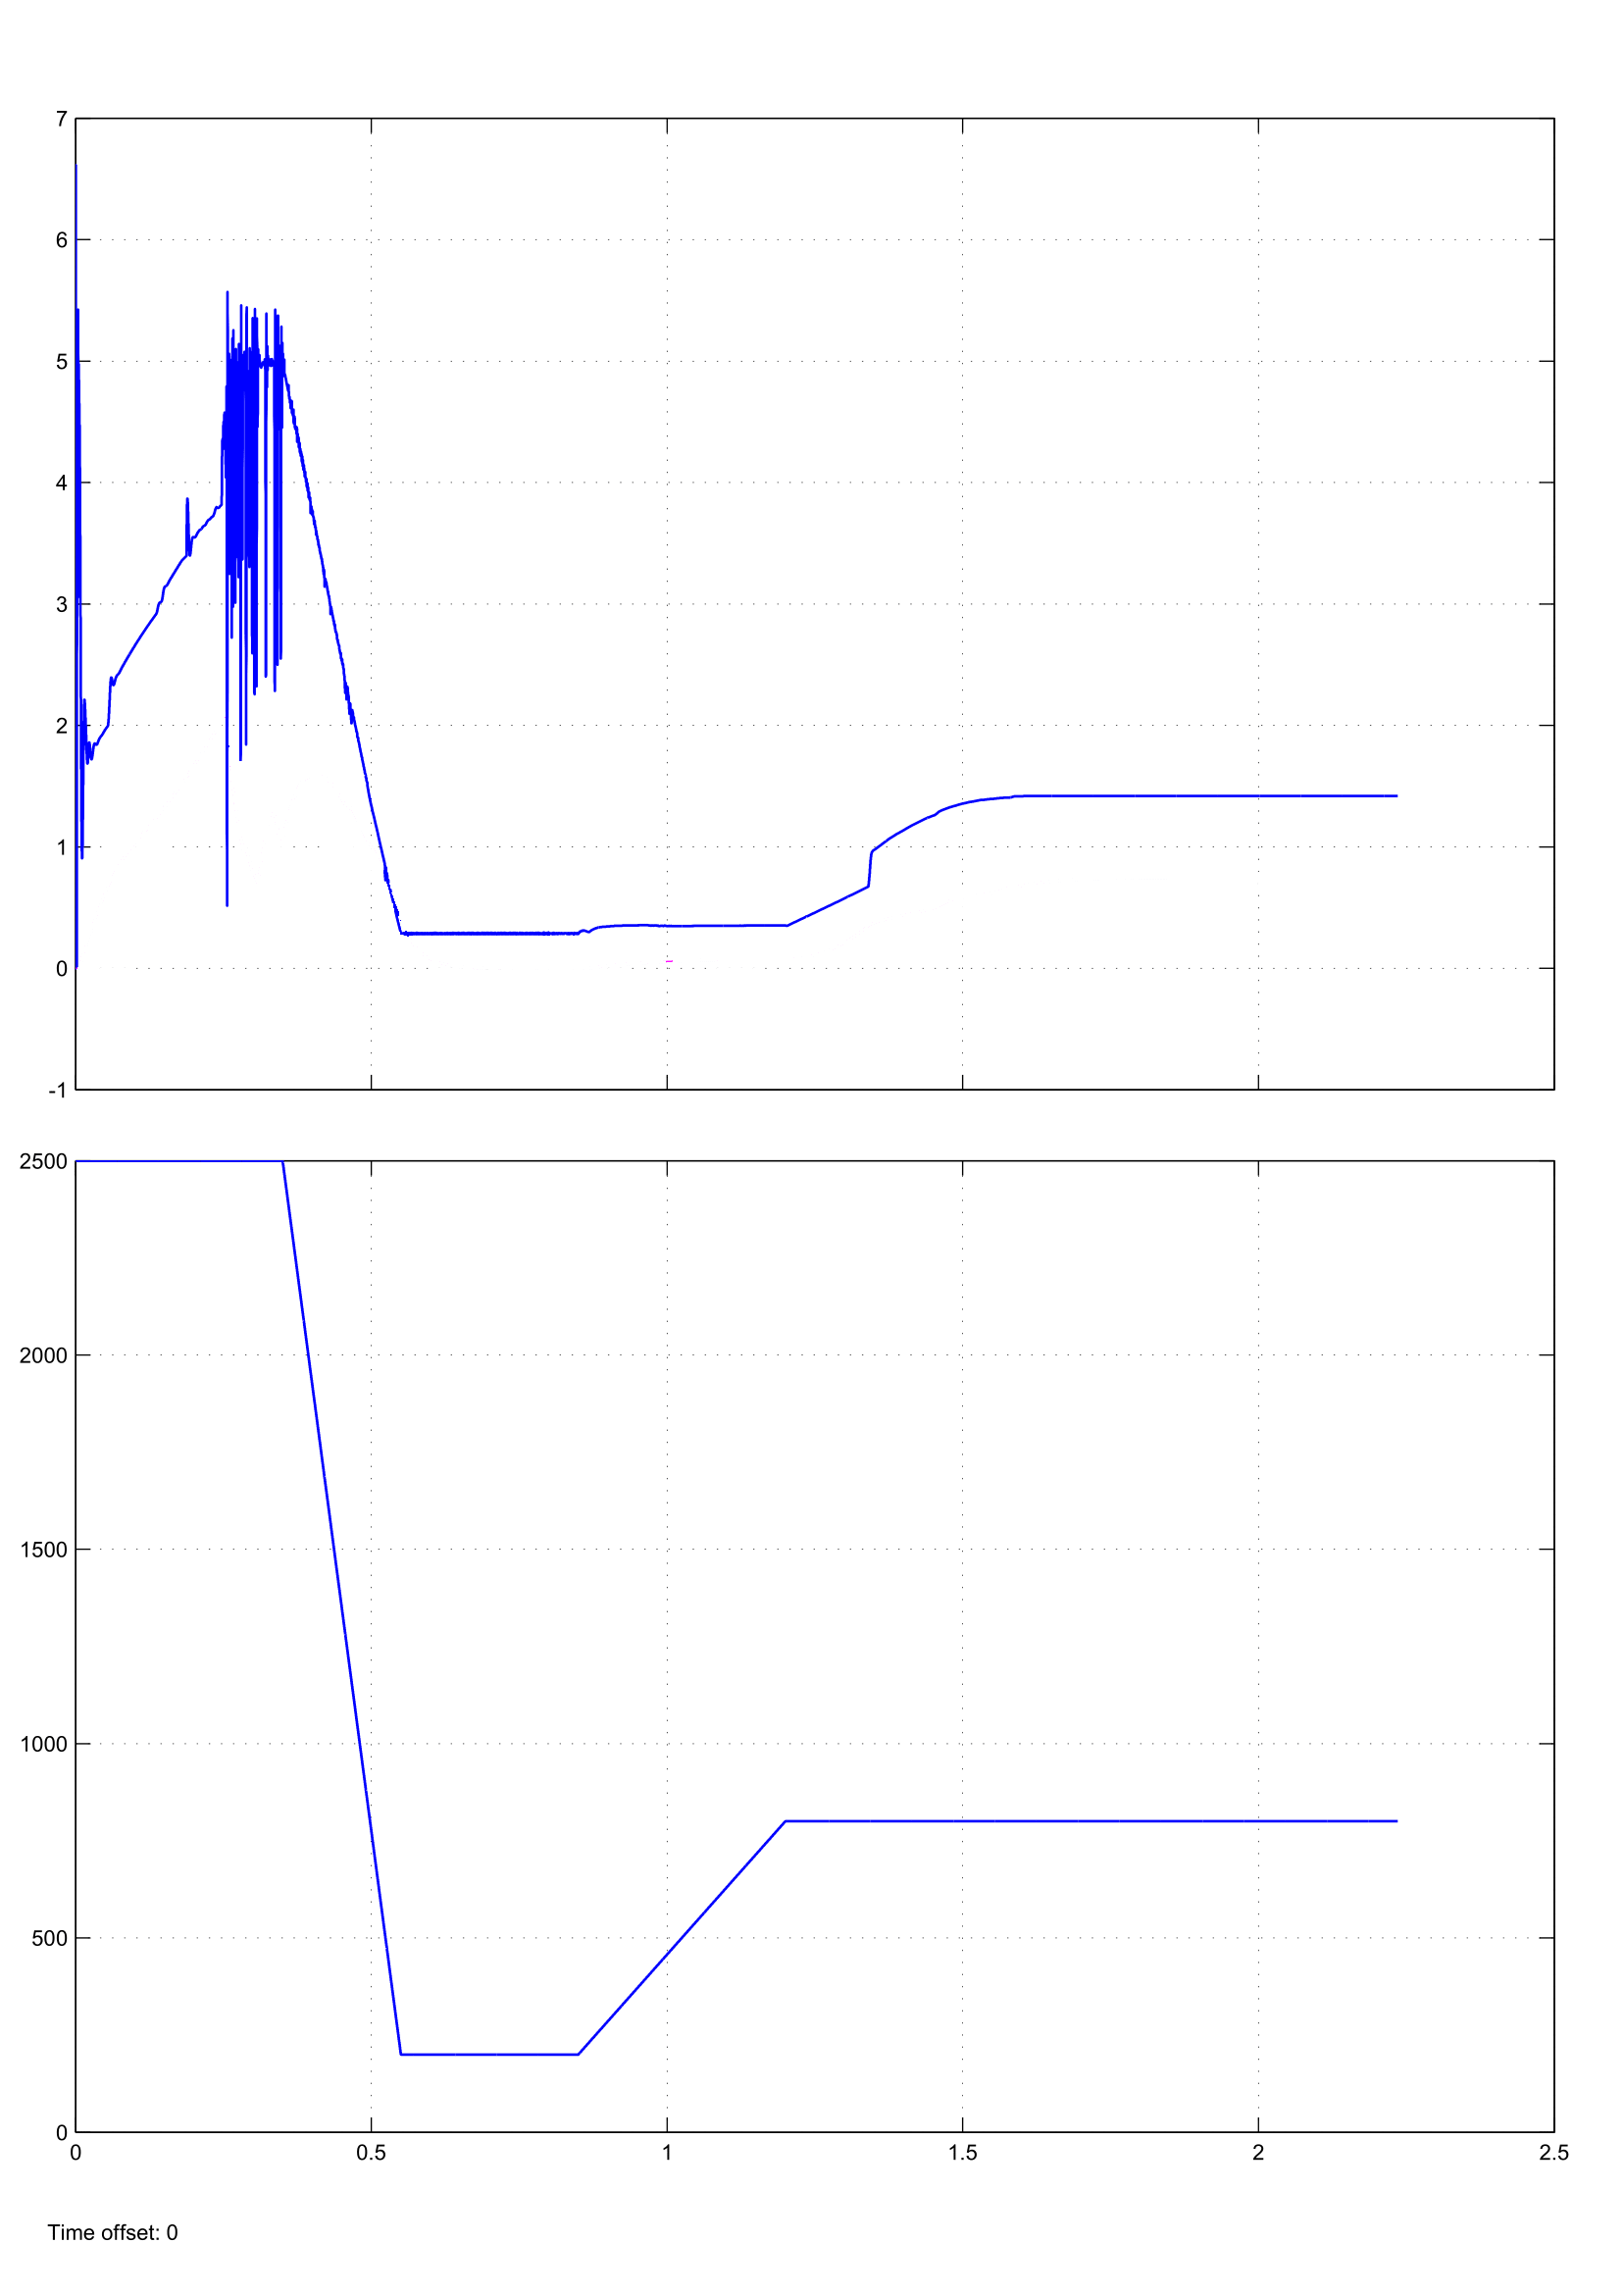
\includegraphics[width=\textwidth]{images/P&O_changing_lux-1}
		   \caption{Perturb and Observe Method on implementation   }
		   \label{fig:PnO_result}
	   \end{center}
   \end{figure}
   
 \section{Incremental Conductance Method }
 
  \begin{figure}[H]
	   \begin{center}
		   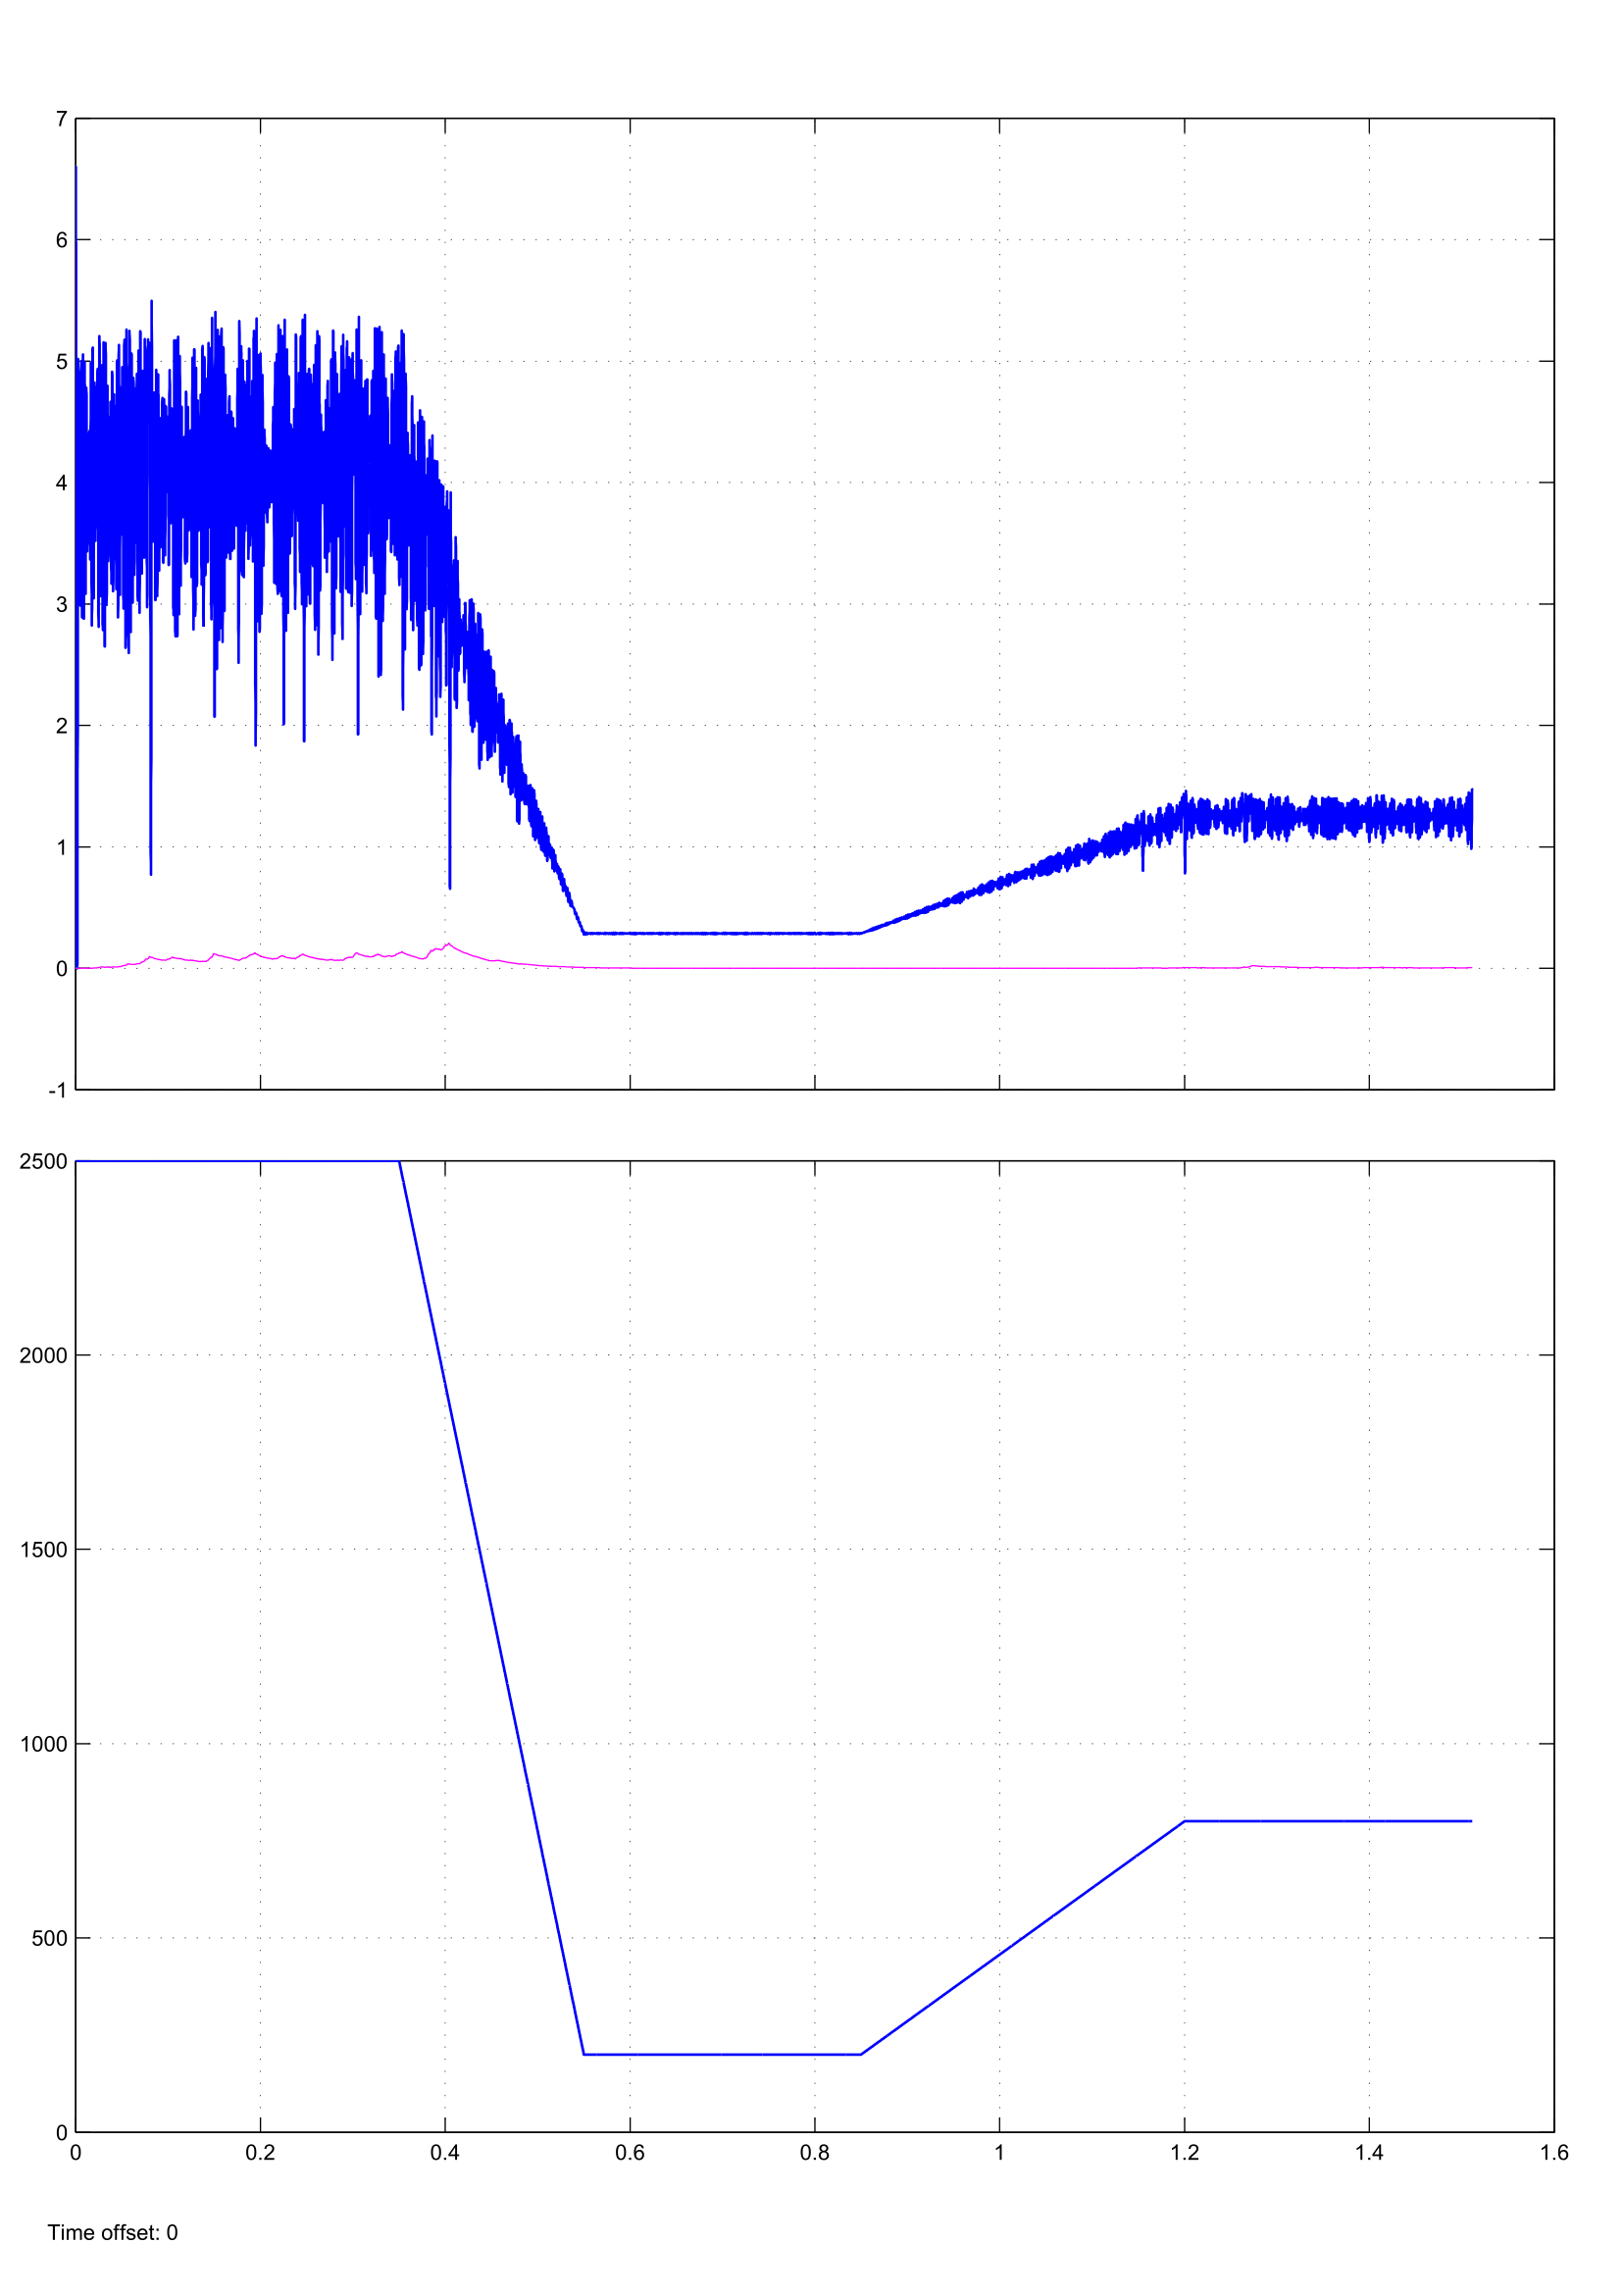
\includegraphics[width=\textwidth]{images/inC_stateflow_changing_lux-1}
		   \caption{Incremental Conductance Method on implementation  }
		   \label{fig:Inc_result}
	   \end{center}
  \end{figure}
 The underlying principle behind \ac{ICM}'s operation is the fact that the slope of the P-V curve is zero when \ac{MPP} is reached. The slope is negative to the right of \ac{MPP} and positive to the left.
 Depending on the direction of the slope $V\textsubscript{ref}$ is moved in steps left or right determined by the sign of the slope. When $V\textsubscript{MPP}$ is reached the cell is held at that potential until a change in $\varDelta$$I\textsubscript{cell}$ is detected.\\
 
 Like in \ac{PnO} the Step size determines how fast \ac{MPP} is reached and its accuracy. Also like before it takes several hundred iterations before \ac{MPP} is reached, leading to longer locking on times - resulting in much lower efficiency. Fixed step size and the several hundred iteration need were the primary reasons \ac{PnO} method and \ac{ICM} were found unsuitable to be used with \ac{DSCs} for \ac{MPPT}. Another argument for not using the two algorithms is that for every iteration two sensors required to be turned, this coupled with the high number of iteration needed; adds up to quite a bit of power used in finding the optimal operating point.             
 
         
 \section{Fractional Open Circuit Voltage Method }
 
As explained in section ~\ref{sec:proposed_algo_sec}, although \ac{FOCV} method has several advantages in terms of simplicity, speed and number of sensors used; the greatest drawback of this method would be its inability of every achieving true \ac{MPP}. By assuming $K_{i}$ as a constant under different illuminations leads to slight loss of power but the simplicity of the circuit helps in reducing its power consumption. This seems to be a fine balance whose odds can be increased by choosing a appropriate value of $K_{i}$. Under simulations, \ac{FOCV} did show a lot of promise by being extremely fast in latching on to $V\textsubscript{MPP}$ with minimal iterations however the power from the cell was always lower than expected. Since under indoor conditions \ac{DSCs} produce minuscule amount of power, any loss would seem significant. The graph for the simulation of\ac{FOCV} looks similar to the one in figure~\ref{fig:Frac_oc_result} on page~\pageref{fig:Frac_oc_result}, key difference being the power levels were lower.             

\section{Proposed Method }

Based on the learnings from simulations and experiments, it was apparent that the selected algorithms would not be the best fit for \ac{DSCs}. Section ~\ref{sec:proposed_algo_sec} makes clear the inner working of the routine. The results are divided into two parts.\\
	
	\begin{enumerate}
		\item Finding \ac{MPP} when the buffer is full.
		\item Locking on to $V\textsubscript{MPP}$ when look-up table is empty or when an out of range $V\textsubscript{OC}$ is detected.				
	\end{enumerate}
In the first condition the sub-routine that is utilized behaves in a manner similar to \ac{FOCV} but deviating by dynamical varying the $K_{i}$ value based on the cell characteristics and past values.    
   \begin{figure}[H]
  	  \begin{center}
  		  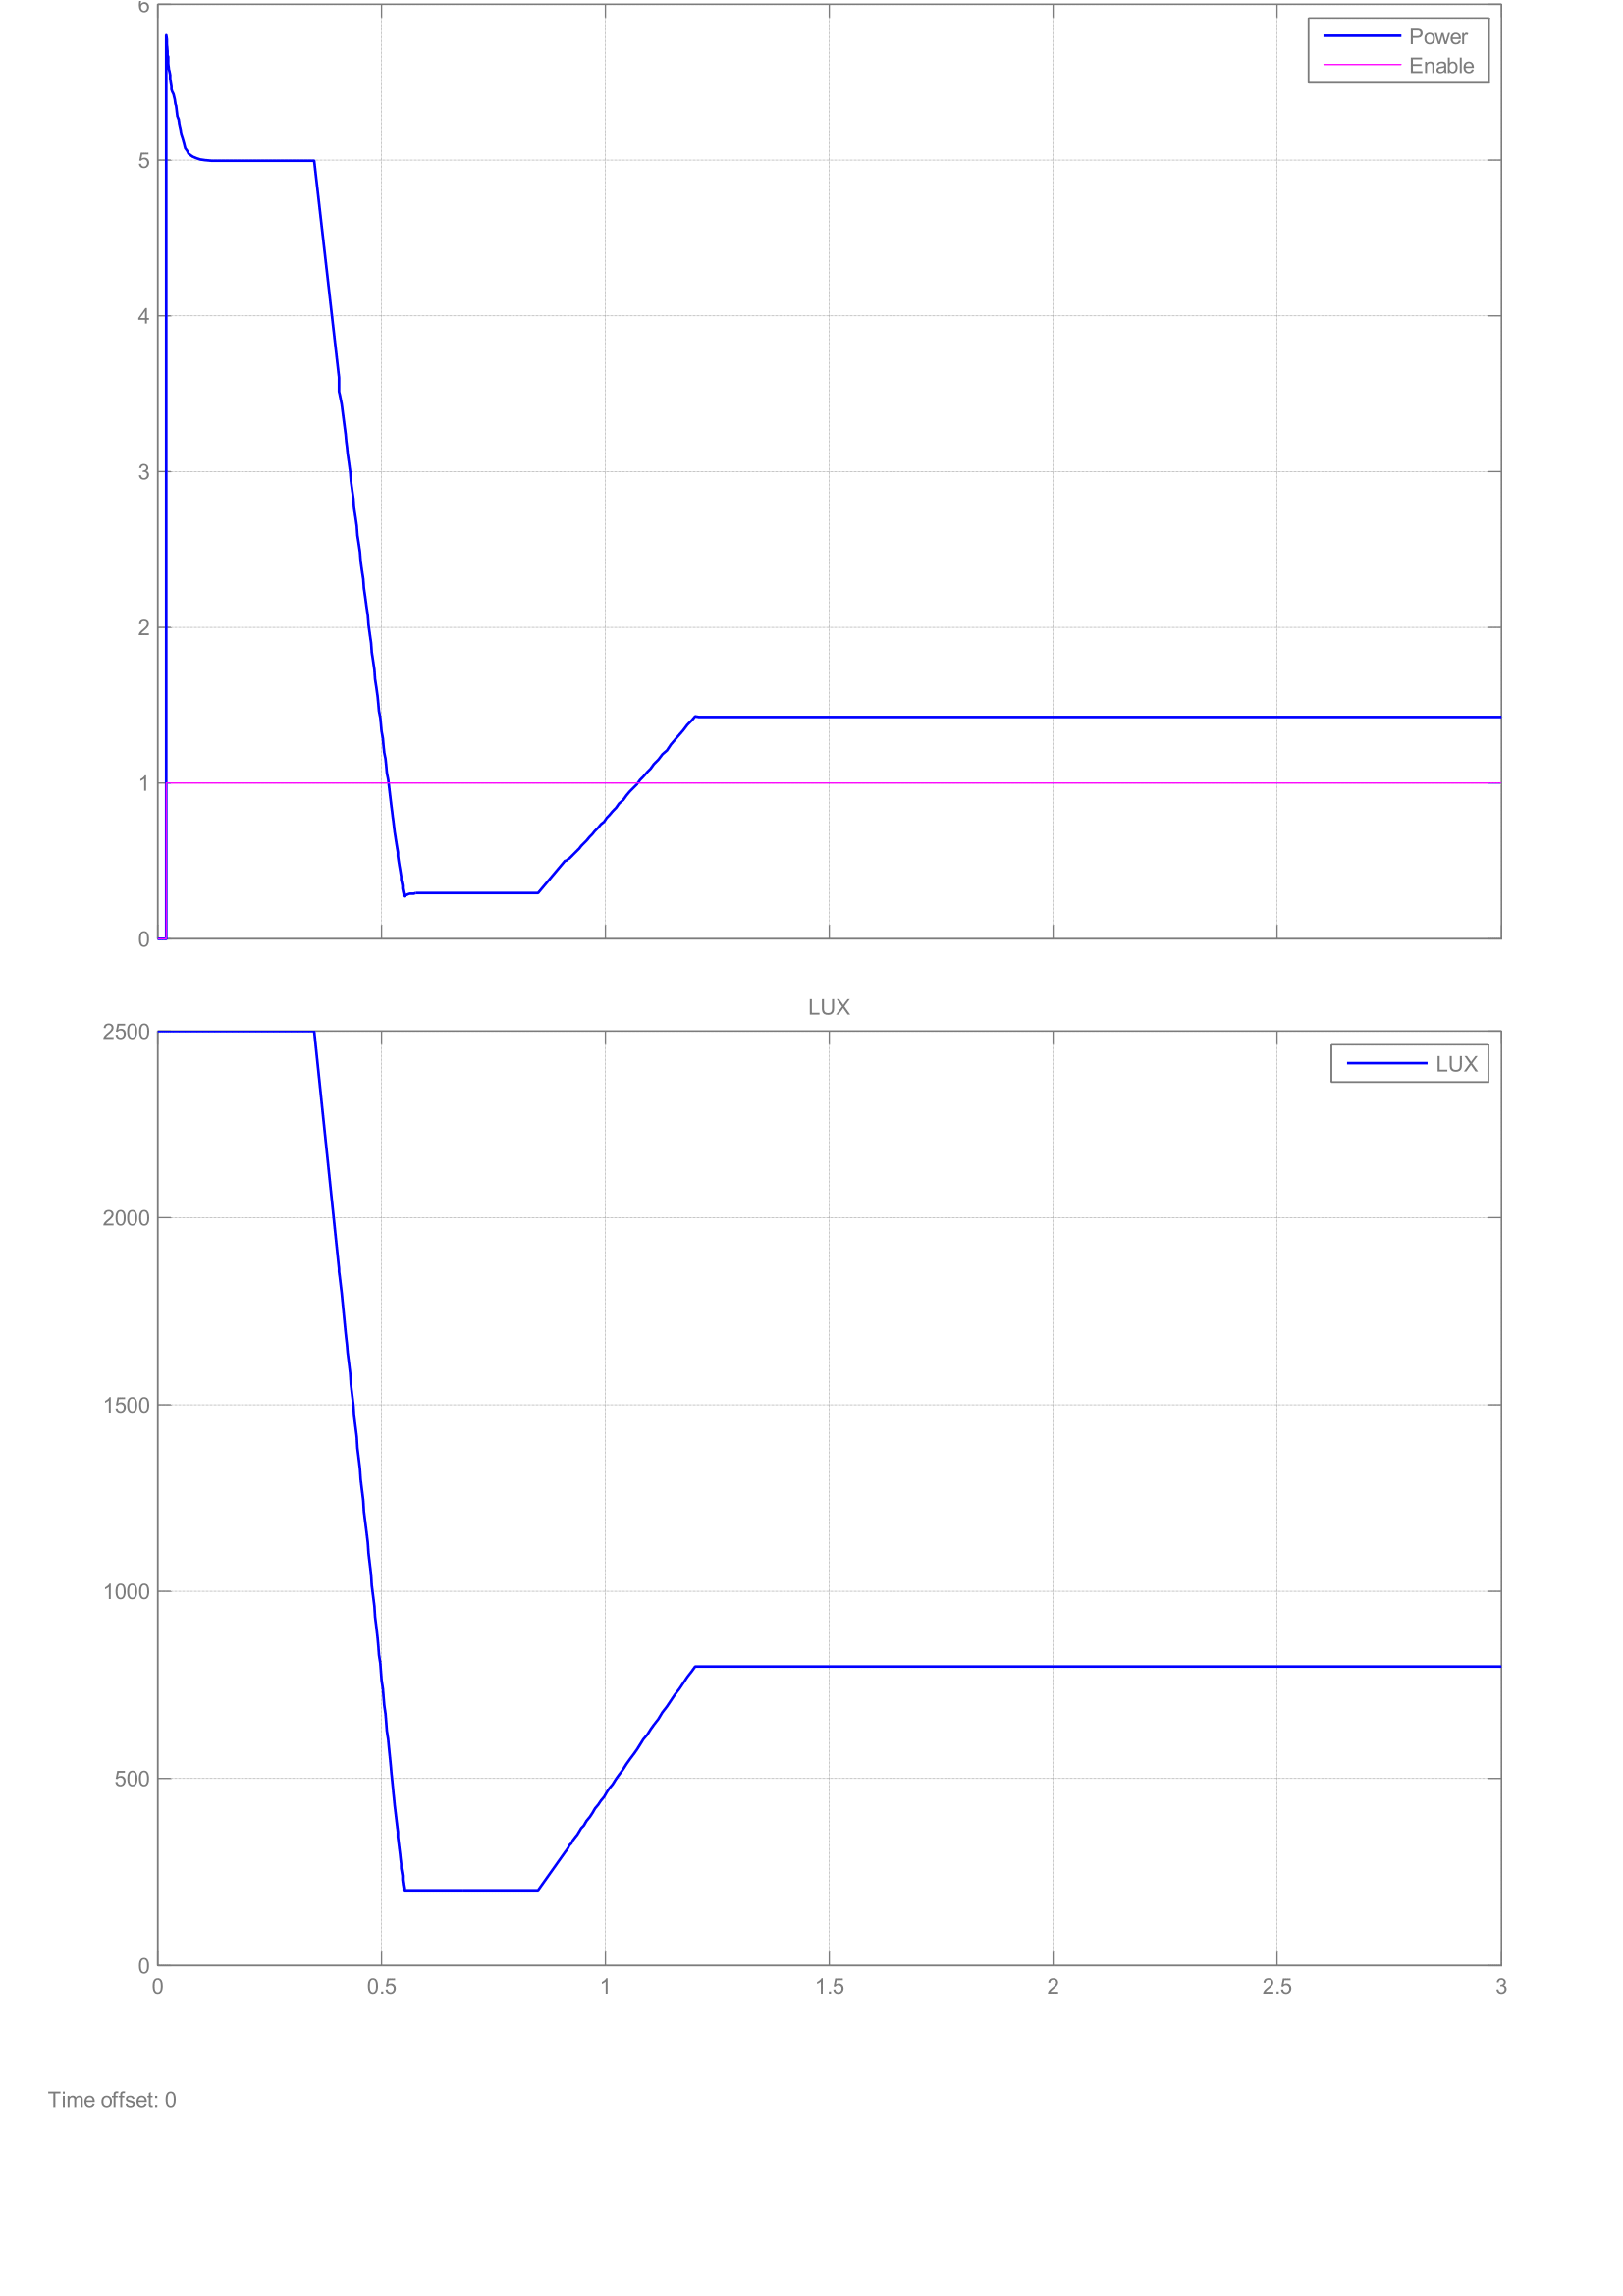
\includegraphics[width=\textwidth]{images/Proposed_algo-1}
  		  \caption{Proposed routine with full buffer, under similar light conditions as other algorithm}
  		  \label{fig:Frac_oc_result}
  	  \end{center}
    \end{figure}

The ability of the algorithm to latch-on to the optimal operating point at great speed is an advantage greatly reducing the power wasted while searching for the \ac{MPP} (power lost due operating the cell on non-optimal potential and power lost due to the active circuitry while searching). The fact that only one sensor, a simple voltage sensing element, is activated for a fraction of a second is an added benefit. Under its typical use case, incident radiation is not expected to vary frequently or by a large degree meaning the \ac{MPPT} controller operates in this sub-routine for majority of the time.\\

For the case where the look-up table is not yet fully populated or when the cell encounters a Lux level that is has not encountered before, a different branch of the algorithm is called. This sub-routine employs \ac{GSSA} to find $V\textsubscript{MPP}$ the search window employed is dynamically  chosen based on previous results in order to reduce the number of iterations required in order to reach the \ac{MPP}.\\

Under Indoor-light conditions, gradual change of illumination is rarely encounter, What we do run up against is more discrete light levels in the form of turning on/off one or more light source in a room. Granted sunlight streaming in from windows does follow a more gradational pattern, this can easily be incorporated in to the controller's design. These discreet Lux levels are a perfect platform to demonstrate the speed at which \ac{GSSA} converges onto the \ac{MPP}.\\

Figure~\ref{fig:proposed_empty_lookup} on page~\pageref{fig:proposed_empty_lookup} depicts output of a controller subjected to discreet light levels starting from 2500 Lux down to 400 Lux. the plot enclosed in the red box is expanded in figure~\ref{fig:Zoom_proposed_empty_lookup} on page~\pageref{fig:Zoom_proposed_empty_lookup}. An enable signal (in pink) was added to indicate start of the search. It is worth noting the speed at which the search algorithm converges on to the Maximum power point. The number of iterations taken before \ac{MPP} was found ,fell between 15 - 20, a far cry from the several hundred needed for \ac{PnO} or \ac{ICM}. This means that even if the cell were to be given a second worth of time to stabilize between iteration the $V\textsubscript{MPP}$ would still be reached within 20 seconds. Consequently this also means the two sensors needed for measuring power would be used a lot fewer times compared to before. \\
       
                     
 \begin{figure}[H]
  \begin{center}
  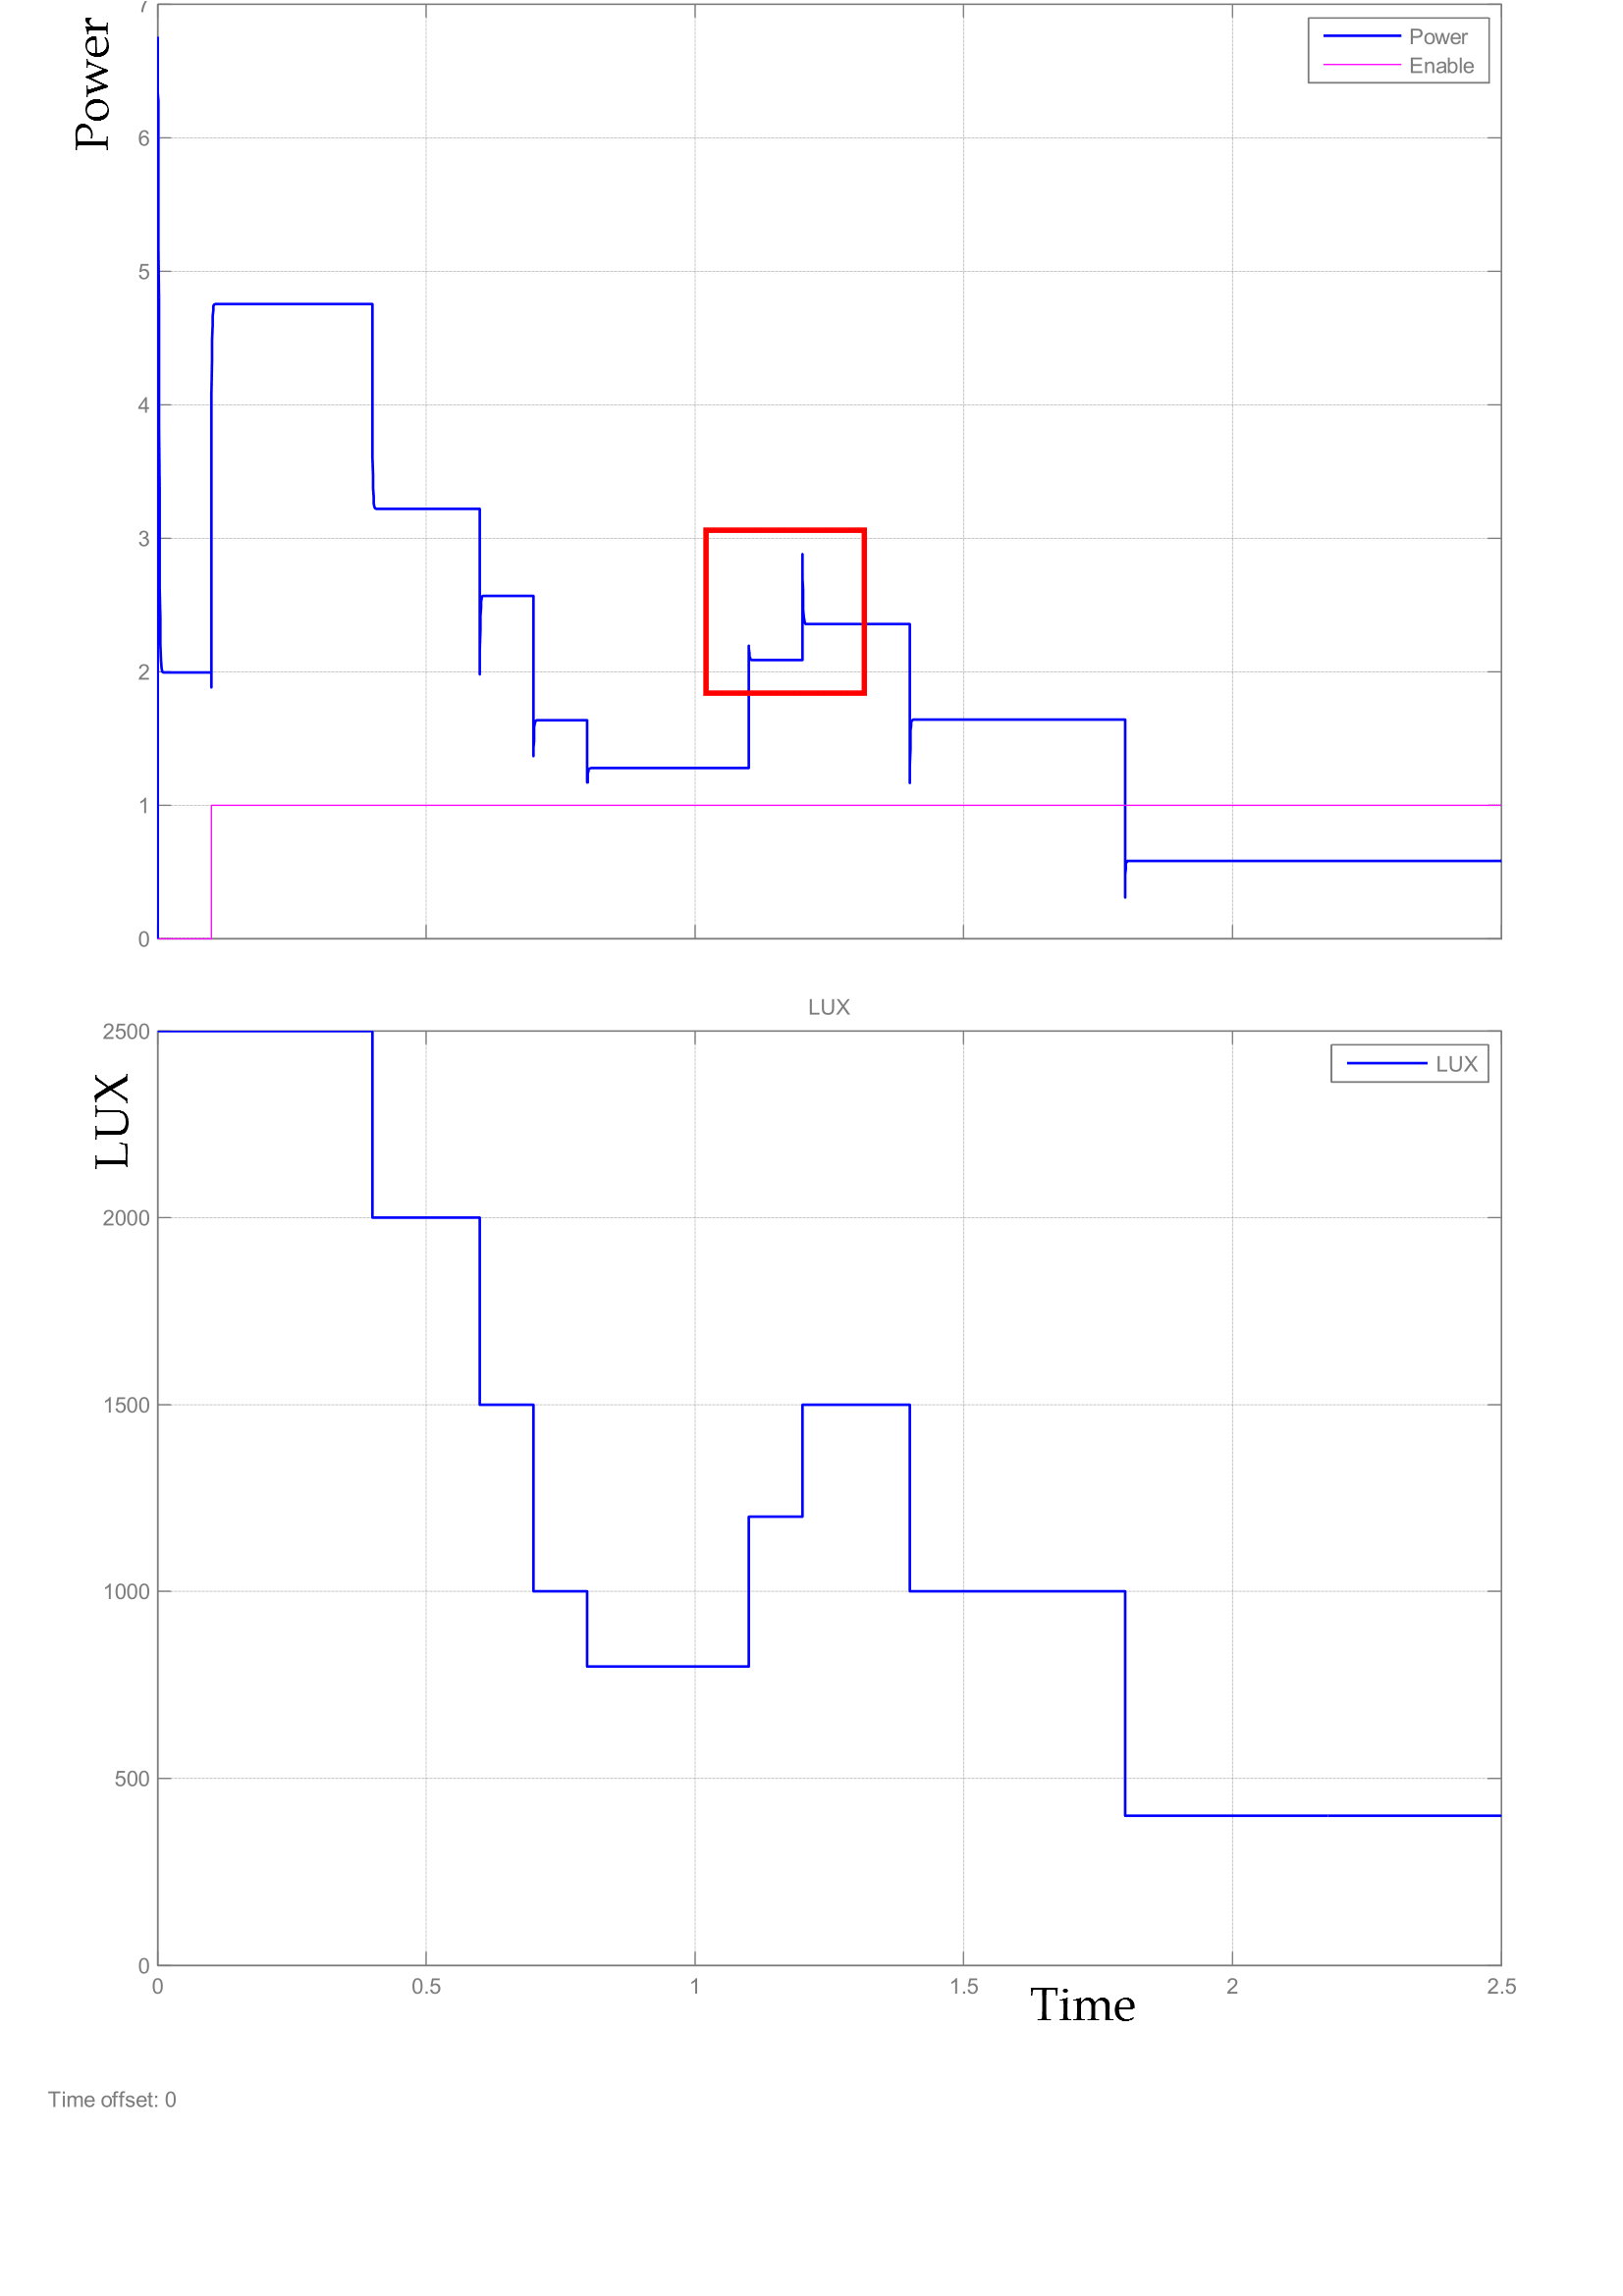
\includegraphics[width=\textwidth]{images/proposed_step_input}
  \caption{Proposed algorithm under rapidly varying light conditions with empty lookup tables }
  \label{fig:proposed_empty_lookup}
  \end{center}
  \end{figure}


 \begin{figure}[H]
  \begin{center}
  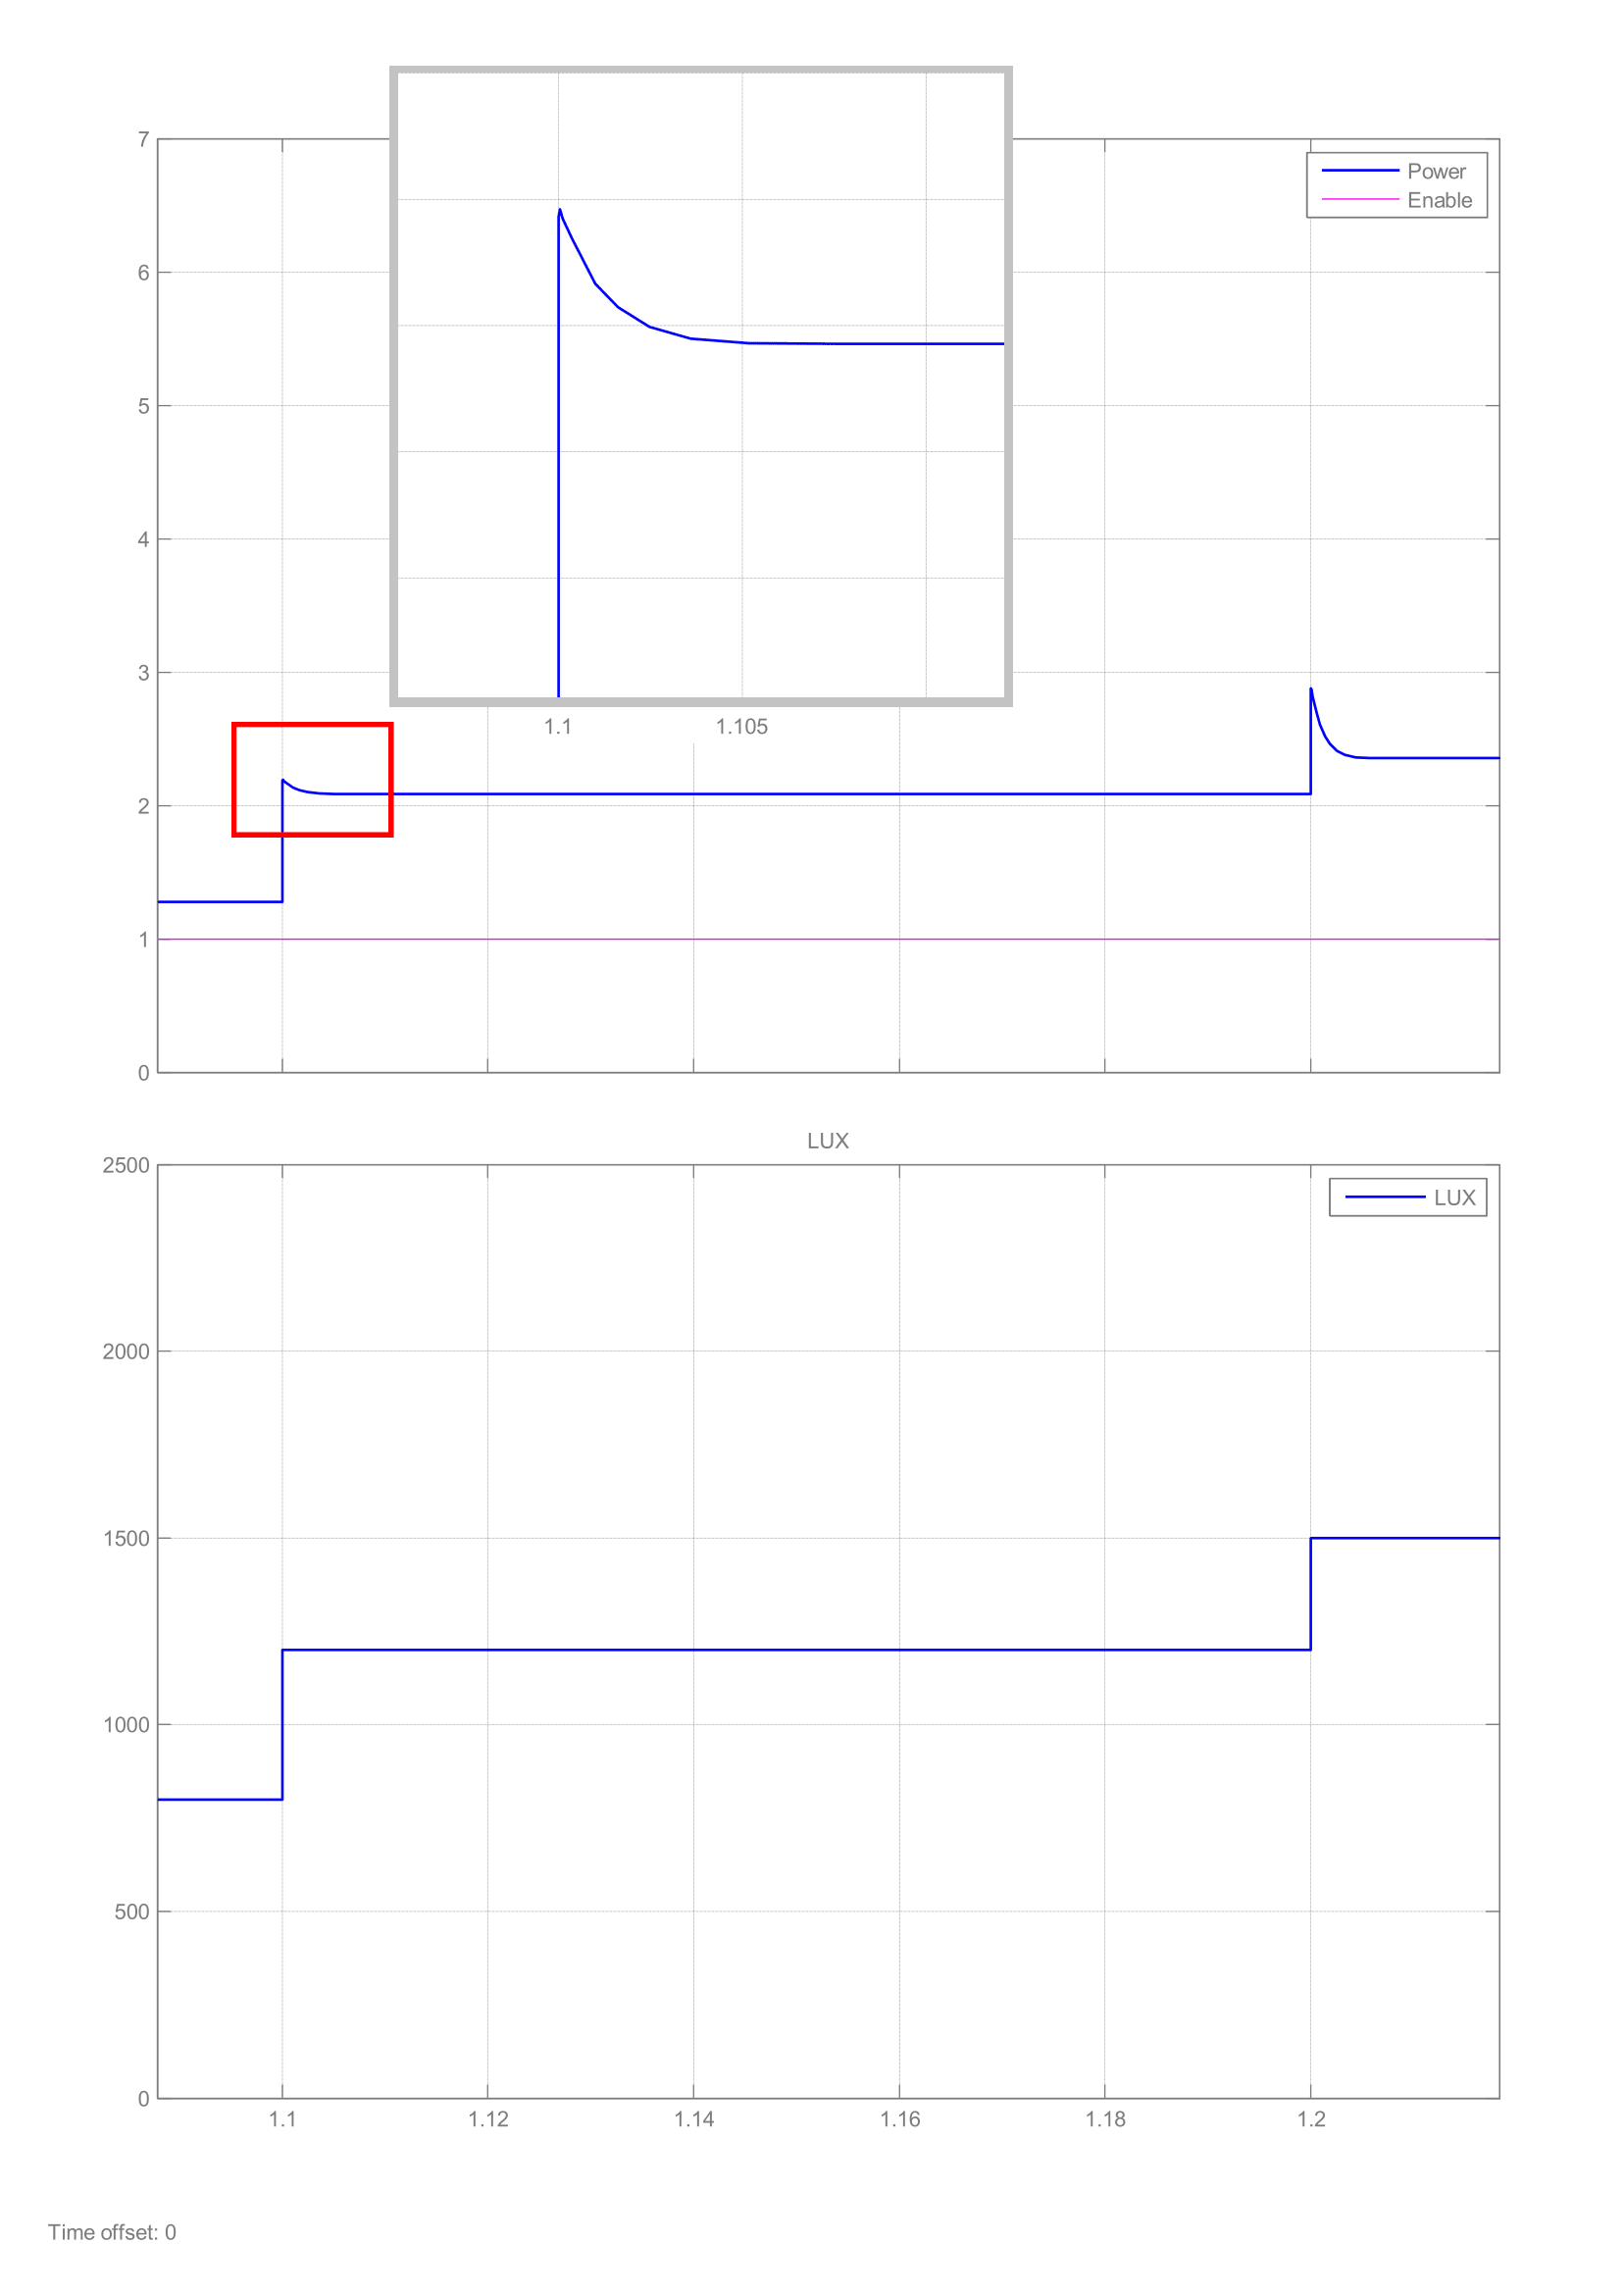
\includegraphics[width=\textwidth]{images/proposed_step_input_zoom-1(2)_pip}
  \caption{ expanded view of the graph in figure ~\ref{fig:proposed_empty_lookup}}
  \label{fig:Zoom_proposed_empty_lookup}
  \end{center}
  \end{figure}

  





	\chapter{Conclusion and Future Work}
\begin{quote} 
\it This final chapter concludes the results obtained from the thesis and attempts to give direction for the future work in this area.
\end{quote}

Several \ac{MPPT} algorithms where studied in relation to this thesis , however only three of the most commercially implemented ones were selected to be tested in this thesis. It was observed that each of the selected algorithms had one or more shortcomings when implemented on \ac{DSCs}, this leads the author to propose his own algorithm best suited for the solar cell at hand. The method shows promise and warrants further study. The author does not discount the fact that there might be several other algorithms in literature that might have an edge with respect to \ac{DSCs} and it could be worthwhile to invest resources to test them out.\\

Several assumptions were made with respect to the model that formed the basis for this research, further efforts could be put into modelling the behaviour based on cell equations. Attempting to extract the unknown cell's parameters could merit a longer look. the model was also based on a solar array in a particular configuration, other configurations/makes of cells should definitely be tried out. That being said the author of the impression that most \ac{MPPT} algorithms are essentially peak finding routines which imply that they would perform in a similar manner independent of the model or IV curves provided. Model based on the simplest diode equation may have indeed been sufficiently accurate within reasonable ranges,giving acceptable results for the purpose of this thesis.\\

Machine learning algorithms implemented are the most basic; smarter garbage collection in the buffer/look up table could improve the accuracy further. The process of formulating a new hybrid algorithm and testing this hypothesis out robbed valuable time that could have be utilised on developing test hardware. \ac{HIL} testing will definitely bring into focus new variables of energy efficiency, sensor count, power budgeting of each measurement, cost of final hardware among others. \ac{HIL} simulations will also show if the assumptions made before still hold water. In essence \ac{HIL} testing is the logical next step for thesis work.\\


    %\chapter{Conclusions And Future Work}

This study presents a base level attempt to find out how much of a user trajectory can be identified by an adversary with higher chance. Prospective non-safety applications in \ac{VANETS} were considered for emulation. These applications aim to provide users with certain
convenience and comfort applications. Though these applications promise to enhance user experience while driving, these also raise a concern towards users' privacy. Privacy analysis of non-safety applications is done and a base skeleton model was designed using heuristic methodology. The skeletal model aids in analysing different non-safety applications and their data exchange statistics between the vehicle and Infrastructure. We simulated realistic vehicular data with \ac{SUMO} simulator and the resultant dataset obtained was further used to emulate the use of non-safety applications. In addition, different adversarial setups and varying non-safety application running times were incorporated. Efforts were taken to replicate a realistic possible scenario.

After carrying out the planned research, results show that more the vehicles are exposed to non-safety application usage, the higher percentage of its trajectory is known to the adversary monitoring the communication channel. In addition, the results also show that an adversary with additional knowledge of crowded and dense road networks can determine significant user trip information. Further research into the topic can take advantage of all the results from the study.

The subjects for future work could include 1) Development of privacy enhancing approach that would provide a suitable balance between user privacy and quality of service for non-safety applications. 2) Real time simulation of vehicular movements, vehicular communication networks and application hosting/running can be carried upon and identifiers affecting the privacy of the user can be investigated. 3) Non-safety application privacy analysis skeletal model developed in this study can be updated with newer findings from the real time simulation as mentioned in point 2. 

    %\bibliographystyle{plain} 
    %\bibliography{bibfile}
	\printbibliography[title=References]
\end{document}
